\documentclass[whitelogo]{tudelft-report}
\usepackage{natbib}
\usepackage{changes}
\usepackage{draftwatermark}
\SetWatermarkScale{1}
\usepackage{verbatim}
\usepackage{hyperref}
\usepackage{color,soul}
\usepackage[english]{babel}
\usepackage{amsthm}
\usepackage[utf8]{inputenc}
\usepackage{latexsym}
\usepackage{amsfonts}
\usepackage{amssymb}
\usepackage{amsmath}
\usepackage{graphicx}
\usepackage{float}

\theoremstyle{definition}
\newtheorem{definition}{Definition}[section]
\theoremstyle{theorem}
\newtheorem{theorem}{Theorem}[section]
\theoremstyle{proposition}
\newtheorem{proposition}{Proposition}[section]
\theoremstyle{corollary}
\newtheorem{corollary}{Corollary}[section]
\theoremstyle{lemma}
\newtheorem{lemma}{Lemma}[section]
\theoremstyle{example}
\newtheorem{example}{Example}[section]
\theoremstyle{remark}
\newtheorem{remark}{Remark}[section]

\DeclareMathOperator*{\argmax}{arg\,max}
\DeclareMathOperator*{\argmin}{arg\,min}

\begin{document}

%% Use Roman numerals for the page numbers of the title pages and table of
%% contents.
\frontmatter

%% Uncomment following 19 lines for a cover with a picture on the lower half only
%\title[tudelft-white]{Title}
%\subtitle[tudelft-cyan]{Optional subtitle}
%\author[tudelft-white]{J.\ Random Author}
%\affiliation{Technische Universiteit Delft}
%\coverimage{cover.jpg}
%\titleoffsetx{10cm}
%\titleoffsety{10cm}
%\afiloffsetx{1cm}
%\afiloffsety{18cm}
%\covertext[tudelft-white]{
%    \textbf{Cover Text} \\
%    possibly \\
%    spanning 
%    multiple 
%    lines
%    \vfill
%    ISBN 000-00-0000-000-0
%}
%\makecover

%% Uncomment following 16 lines for a cover with a picture on the lower half only
\title[tudelft-white]{Sybil-proof Accounting Mechanisms in P2P Networks}
% \subtitle[tudelft-black]{Optional subtitle}
\author[tudelft-white]{Alexander\ Stannat}
\affiliation{Delft University of Technology}
\coverimage{tank.jpg}
%\covertext[tudelft-white]{
%    \textbf{Cover Text} \\
%    possibly \\
%    spanning 
%    multiple 
%    lines
%    \vfill
%    ISBN 000-00-0000-000-0
%}
%\setpagecolor{tudelft-cyan}
\makecover[split]


%% Include an optional title page.
\begin{titlepage}


\begin{center}

%% Insert the TU Delft logo at the bottom of the page.

%% Print the title in cyan.
{\makeatletter
\largetitlestyle\fontsize{64}{94}\selectfont\@title
%\largetitlestyle\color{tudelft-cyan}\Huge\@title
\makeatother}

%% Print the optional subtitle in black.
{\makeatletter
\ifx\@subtitle\undefined\else
    \bigskip
   {\tudsffamily\fontsize{22}{32}\selectfont\@subtitle}    
    %\titlefont\titleshape\LARGE\@subtitle
\fi
\makeatother}

\bigskip
\bigskip

by
%door

\bigskip
\bigskip

%% Print the name of the author.
{\makeatletter
%\largetitlefont\Large\bfseries\@author
\largetitlestyle\fontsize{26}{26}\selectfont\@author
\makeatother}

\bigskip
\bigskip

to obtain the degree of Master of Science
%ter verkrijging van de graad van Master of Science

at the Delft University of Technology,
%aan de Technische Universiteit Delft,

to be defended publicly on Tuesday January 1, 2013 at 10:00 AM.
%in het openbaar de verdedigen op dinsdag 1 januari om 10:00 uur.

\vfill

\begin{tabular}{lll}
    Student number: & 1234567 \\
    Project duration: & \multicolumn{2}{l}{March 1, 2012 -- January 1, 2013} \\
    Thesis committee: & Prof.\ dr.\ ir.\ J.\ Doe, & TU Delft, supervisor \\
        & Dr.\ E.\ L.\ Brown, & TU Delft \\
        & Ir.\ A.\ Aaronson, & Acme Corporation
\end{tabular}
%% Only include the following lines if confidentiality is applicable.

\bigskip
\bigskip
\emph{This thesis is confidential and cannot be made public until December 31, 2013.}
%\emph{Op dit verslag is geheimhouding van toepassing tot en met 31 december 2013.}

\bigskip
\bigskip
An electronic version of this thesis is available at \url{http://repository.tudelft.nl/}.
%\\[1cm]

%\centering{
\includegraphics{cover/logo_black}}


\end{center}

\begin{tikzpicture}[remember picture, overlay]
    \node at (current page.south)[anchor=south,inner sep=0pt]{
        
\includegraphics{cover/logo_black}
    };
\end{tikzpicture}

\end{titlepage}


\chapter*{Abstract}
\label{chap:Abstract}

Online P2P file sharing networks rely on the cooperation of participants to function effectively. Agents up- and download files to one another without the need for any central authority. If agents all contribute to the network and share roughly the same amounts of data as they contribute the network will operate, however if some agents decide to defect and consume far more resources than they contribute the file sharing will stagnate. In online networks with some kind of central authority, such as Ebay, Airbnb, etc. cooperation is achieved through a review system, which is maintained and secured by the central authority. P2P networks are however distributed and cooperation must be achieved without this central mitigator. One way of approaching this problem is by observing cooperative biological communities in nature. One finds that cooperation among biological organisms is achieved through a mechanism called indirect reciprocity. Indirect reciprocity is based on a reputation scheme in which agents share information about each other's cooperativeness aiding one another in deciding who to interact with and who to shun. In this work we analyse properties a reputation mechanism must satisfy in order to achieve cooperation in P2P networks, incentivising contributions and penalising excessive comsumption of data. In particular, we determine under what conditions reputation mechanisms are resistant to attacks on the P2P network. We focus on one attack above all, namely that of a sybil attack in which a malicious agent creates multiple fake identities who report high levels of cooperativeness about one another. We determine properties accounting mechanisms must satisfy in order to prevent attackers from obtaining arbitrarily high reputation and to consequently be able to consume arbitrarily large amounts of data. This thesis offers a theoretical framework for evaluating the effectiveness of reputation mechanisms on the basis of their ability to induce cooperation and their resistance to sybil attacks.


\chapter*{Preface}
\setheader{Preface}

Preface\ldots

\begin{flushright}
{\makeatletter\itshape
    \@author \\
    Delft, January 2013
\makeatother}
\end{flushright}



\tableofcontents

%% Use Arabic numerals for the page numbers of the chapters.
\mainmatter
\chapter{Introduction}
\label{chap:Introduction}



\noindent{}Honest cooperation in a population is a requirement for any level of organisation to be reliably reached. From genes, unicellular organisms, and multicellular organisms to insect colonies and human societies, the ability to cooperate is of vital importance for the survival of these species. Interactions between agents in a population can be viewed as instances of evolutionary game theory. Each interaction places two agents together whereby one agent needs the other to contribute some resource to them. Here a resource is defined in an abstract sense as any kind of helpful act that contributes to the chance for survival of a peer. This is an altruistic act of the individual, but a requirement for the survival of the entire population.\vspace{1em}\\


\section{The Evolution of Social Cooperation}
\label{sec:The Evolution of Cooperation}
\noindent{}Natural selection engenders competition among agents in a population such that selfish behaviour is rewarded. This can lead to a dilemma, commonly known as the "tragedy of the commons", in which the incentives of the individual are not aligned with those of the population as a collective. Such a dilemma is partially thwarted by the evolution of a number of mechanisms that induce cooperation in a population. Without any mechanism for the evolution of cooperation, natural selection favors defectors, which consequently outlive honest agents until there are only defectors left. Research has shown that there are 5 predominant mechanisms that biological communities adopt in order to maintain cooperation, namely {\it kin selection}, {\it direct reciprocity}, {\it indirect reciprocity}, {\it network reciprocity} and {\it group selection}. The idea behind these particular mechanisms is to reward behaviour of individuals that is beneficial to members of the population other than themselves and to some degree even punish "selfish" behaviour \cite{5 Rules for the Evolution of Cooperation}.\vspace{1em}\\


\noindent{}Agents in a population will incur some cost for performing an altruistic act, while the recipient will receive some benefit. Different mechanisms of social cooperation will yield different cost and benefit functions for altruisitc acts, based on which agents will decide whether or not it is sensible for them to cooperate. Nowak (2006) have determined under which restrictions of cost and benefit, cooperation will naturally evolve in biological communities.\vspace{1em}\\

\begin{itemize}
\item Kin Selection: Natural selection can favour cooperation if contributer and beneficiary are genetic relatives. Such an act is beneficial if the cost-to-benefit ratio exceeds the factor of relatedness, whereby the factor of relatedness is determined by the probability that both interaction partners share a gene. 
\item Direct Reciprocity: In the case of repeated encounters between the same individuals with consecutive rounds of interactions, an agent will decide whether to cooperate based on its contender's previous action. The most common form of direct reciprocity is known as the tit-for-tat strategy in game theory, which we will elaborate on later. Direct reciprocity leads to global cooperation if the cost-to-benefit ratio is exceeded by the probability of another interaction between the same agents.
\item Indirect Reciprocity: In indirect reciprocity a node cannot rely on reencountering one of its previous interaction partners, but instead is likely to encounter strangers over and over again. %resembles a barter economy, Indirect reciprocity is similar to money.
This necessitates a mechanism that works on the basis of reputation. Agents may not have the chance to reciprocate directly. Instead, people contribute to the community on the assumption that it will increase their reputation, which in turn increases the probability of them receiving some work from a stranger. This mechanism only induces cooperation if the probability of knowing someone's reputation exceeds the cost-to-benefit ratio of the interaction.
\item Network Reciprocity: We can picture this best in a graph-theoretical setting, in which every agent pays a cost for all of their neighbours in the social graph to receive a benefit. If they defect then their neighbours don't receive a benefit. Cooperators can prevail by forming network clusters among themselves, by only interacting with cooperators. This rule leads to cooperation if benefit-to-cost ratio exceeds the average number of neighbours each node has. 
\item Group Selection: The network is subdivided into groups and these groups grow as offspring is produced. As a group reaches a certain size  it splits in two and another group is eliminated. We find that defectors in a mixed group proliferate faster than honest nodes. However, groups consisting of only honest nodes split much faster than mixed groups or groups with only defectors. Hence honest groups soon dominate the network. This only happens provided that the benefit-to-cost ratio is greater than the ratio of all nodes to number of groups plus 1. \vspace{1em}\\
\end{itemize}

\noindent{}Out of all biological species there are on this planet, the human race has developed the by far most sophisticated and effective mechanism to enforce indirect reciprocity across its entire population; Language. While many other life forms on earth have developed ways of communicating with one another, humans have developed the most intricate and complex method of communication. This is the reason that from an evolutionary perspective, we have arguably outdone all other biological species on this planet. Language enables humans to {\it gossip} about one another. While this might not initially seem like a significant contributor to reproductive success, it allows humans to share information about the reliability of their peers and the likelihood that an individual will act cooperatively in the future. Based on this shared information humans can cultivate a reputation which reflects their standing in a population.  \vspace{1em}\\

\noindent{}This reputation mechanism rewards altruistic behaviour and punishes uncooperative acts. If, in an interaction with a peer an agent decides to defect then that peer will spread information about the agent's defection and if said agent has another interaction with a new peer that knows about its past defection then the agent is less likely to be collaborated with. Humans have developed an awareness of their own reputation over time which prompts them to behave cooperatively most of the time. Even with strangers whose reputation they might not know, humans often act politely and considerately, due to this awareness. While kin selection and direct reciprocity can ensure the cooperation of smaller tribes and families, reputation is a key element in the functioning of large-scale societies. \vspace{1em}\\

\noindent{}The upshot here is that bad behaviour is punished with bad reputation, while good behaviour is rewarded with good reputation. Good reputation leads to trust between two individuals, which results in more effective cooperation between individuals. Lastly, humans have incorporated "forgiveness" into this scheme. Individuals' reputations are malleable and dynamic. Agents that have misbehaved and developed a bad reputation can change their behaviour and redeem themselves, correcting their wrong-doings and fixing their reputation. This upgrades the reputation mechanism and ensures that defectors are incentivised to rectify their strategy and become cooperators.\vspace{1em}\\


\section{Cooperation and Behaviour on the Internet}
\label{sec:Cooperation and Behaviour on the Internet}
\noindent{}With the advent of one of the most disruptive technological revolutions in human history, namely the Internet, humans have been given an entirely new platform to interact on globally. There are a wide variety of different networks in which different types of resources are shared, from P2P file sharing networks, where agents up- and download data to one another to social networks where humans interact by sharing content with one another and rewarding or chastising it with "likes" or "retweets", etc. The social graph of human interaction has changed and especially grown significantly with the help of these tools. This changes the paradigm of human interaction and consequently their behaviour. It has been commonly observed that people are often much "nastier" to one another on the Internet than they are in real life. This nastiness can be considered as a form of defection against paradigms of social interaction, leading us to believe that the aforementioned rules for inducing cooperation no longer function effectively.\vspace{1em}\\

\noindent{}On the Internet humans no longer interact face-to-face and, more importantly, no longer need to disclose their identity to one another. Identity, however is an indispensable input of any reputation mechanism. For a reputation mechanism to be effective, identities need to be permanent and unique. When humans have the ability to hide their identity behind one or several pseudonyms, they can defect without having to face any long-term repercussions. Malicious peers may hide behind one or several pseudo-identities or even erase previous identities entirely in order to avoid bad reputation as a result of bad behaviour. The regular mechanisms for cooperation are no longer applicable and a new online analogue to reputation might have to be devised. This problem becomes particularly apparent in online social networks.\vspace{1em}\\

\noindent{}Social networks such as Facebook and Twitter, etc. struggle to clamp down on malicious behaviour such as cyberbullying and the proliferation of hateful content or "fake news". In the physical world this type of behaviour would be strongly disincentivised by the mechanisms of cooperation given in \ref{sec:The Evolution of Cooperation}. A bully for instance, will be socially frowned upon and become an outcast from the community if their behaviour is not rectified. Of course, even in the real world these cooperative mechanisms are not implemented perfectly, however they do work. On the Internet, due to the reasons discussed above, we find that this is no longer the case. Reputation is no longer a reliable piece of information and trust is harder to achieve, making these networks increasingly uncooperative environments. While companies running these networks do their best in utilising technology to prevent and mitigate bad behaviour, they have so far not succeeded entirely.\vspace{1em}\\ 


\section{Cooperation in Peer-to-peer Filesharing Networks}
\label{sec:Cooperation in Peer-to-peer Filesharing Networks}
\noindent{}Another preeminent setting in which this problem of cooperation arises are online P2P filesharing networks. Peer-to-peer file sharing refers to the distribution of digital media over a P2P network without the need for any central authority or database. Files are located on individuals' computers and shared with other members of the network through up- and downloading data to one another. P2P software was the piracy method of choice in the early 2000s with software programmes such as LimeWire, Gnutella and the BitTorrent client being the most prominent applications \cite{The Early Days of Mass Internet Piracy Were Awesome Yet Awful}. A Supreme Court decision in 2005 led to the closure of many of these sites for illegally sharing copyrighted material. However, these applications are still very much in use today.\vspace{1em}\\

\noindent{}In P2P file sharing networks agents up- and download files amongst one another through acts called {\it seeding} and {\it leeching}. Agents holding a particular file will receive requests for the given file they are holding by so-called leechers. Nodes that require a particular file join a swarm of other nodes with the same needed file. Agents willing to seed now have to decide who to make a contribution to. The file they are willing to share is split into smaller pieces which are distributed among members of the swarm in a manner that ensures a fair distribution and prevents data from going extinct when agents go offline or leave the mesh. \vspace{1em}\\

\noindent{}P2P filesharing networks are an instance of computing distributed systems, which do not have any central authority governing the network. Instead of connecting to a central server for data, agents interact freely in a decentralised manner as visualised in figure \ref{fig:Client-Server vs P2P Model}. \vspace{1em}\\


\begin{figure}[H]
\begin{center}
\includegraphics[scale=0.75]{"Central vs Decentralised".PNG}
\caption{Client-Server vs P2P Model}
\label{fig:Client-Server vs P2P Model}
\end{center}
\end{figure}

\noindent{}There are some advantages and some disadvantages of the distributed nature of P2P networks over the traditional client-server model and their applicability depends on the context. The most notable are listed in the table given in figure 1.2 below.\vspace{1em}\\

\begin{figure}[H]
\begin{center}
\begin{tabular}{|c|c|}
\hline & \\[-0.7ex] \textbf{Advantages:} & \textbf{Disadvantages:} \\[1.5ex] \hline & \\[0.7ex]
No single point of failure & No Accountability \\
No network congestion & Possible malware on the network \\
No expensive server architecture needed  & No backup of data \\
 & Updates are difficult to implement \\[1ex] 
\hline
\end{tabular}
\label{fig:Pros and Cons of P2P}
\caption{Advantages and disadvantages of P2P over Client-Server}
\end{center}
\end{figure}

\noindent{}In most online networks with some kind of central authority, such as Ebay, Airbnb, etc. cooperativeness is achieved through review mechanisms, which are maintained and secured by the central authority. Agents can evaluate the trustworthiness of their potential interaction partners, by assessing their previous transactions and other agents' opinions of them. These reviews are stored on a central database which the central authority maintains. Seeing as the point behind P2P networks was to eliminate this central authority the problem of cooperation arises again. Users have an obvious incentive to download, but no inherent incentive to share data. This is what we referred to earlier as {\it the tragedy of the commons}, which results in behaviour we call {\it lazy freeriding}, where agents leech excessively, but do not seed. Different file sharing platforms have different mechanisms to enforce the necessary altruistic sharing of files. \vspace{1em}\\


\subsection{BitTorrent \& Direct Reciprocity}
\label{subsec:BitTorrent & Direct Reciprocity}
\noindent{}To facilitate cooperation the most prominent P2P network, BitTorrent, employs a mechanism called {\it tit-for-tat}, which is an instance of direct reciprocity. Tit-for-tat is a highly effective strategy in game theory for the iterated prisoner's dilemma, in which an agent cooperates first and then replicates its contender's previous actions as seen in figure \ref{fig:Instance of the Prisoner's Dilemma, in which Tit-For-Tat is the Dominant Strategy}. In practice, this works as follows. Peers in the BitTorrent network have a limited number of upload slots to allocate. An agent will begin by exchanging upload bandwidth for download bandwidth with a number of its peers. If one of these peers turns out to be a leecher, i.e. does not reciprocate, it will be choked out. This means the agent will discontinue it's cooperation and assign the corresponding upload slot to another randomly chosen peer in a procedure known as {\it optimistic unchoking}. \vspace{1em}\\

\begin{figure}[H]
\begin{center}
\includegraphics[scale=0.7]{"Tit-4-Tat".jpg}
\caption{Instance of the Prisoner's Dilemma, in which Tit-For-Tat is the Dominant Strategy. Image taken from \cite{Prisoner's Dilemma Image}.}
\label{fig:Instance of the Prisoner's Dilemma, in which Tit-For-Tat is the Dominant Strategy}
\end{center}
\end{figure}

\noindent{}However, we find that in the case of fleeting and asymmetric interactions, tit-for-tat is no longer very effective \cite{A Simple Rule for the Evolution of Cooperation on Graphs and Social Networks}. Fleeting and asymmetric means that agents have many unrepeated and unreciprocable interactions with their peers. When there is a high probability of two agents not seeing each other again, peers cannot be evaluated based on their previous reliability and hence every new transaction entails the risk of the contender defecting. In tit-for-tat agents do not keep a memory about their peers' reliability and do not share information about this behaviour with the network. In such a setting defecting becomes the dominant strategy of the Prisoner's dilemma \cite{An Optimal Strategy to Solve the Prisoner's Dilemma}. The agents' inability to coordinate and build expectations of their counterparts ensures that defection will rarely be punished. Everyone is worse off than if they had collaborated, but no individual can gain anything by changing to a collaborative strategy, since there's almost never a reward. This is what we referred to as the tragedy of the commons earlier in section \ref{sec:The Evolution of Cooperation}. We find that a mechanism of indirect reciprocity may be more successful at inducing cooperation in these types of networks. \vspace{1em}\\


\subsection{Tribler \& Indirect Reciprocity}
\label{subsec:Tribler & Indirect Reciprocity}
\noindent{}The {\it Distributed Systems Group} at Delft University is running and developing an open-source P2P file sharing network, called {\it Tribler}, which aims to leverage the power of mechanisms for social cooperation in an attempt to create a more reliable file sharing platform. It is designed with a custom built-in onion routing network whereby the transference of data is routed through several relay nodes before reaching the leeching node, ensuring anonymity of participants and clients can participate in any BitTorrent network. Tribler is trackerless and built on an overlay network for content searching, rendering it truly decentralised and immune to limiting external action such as government restraint.  \vspace{1em}\\ 

\noindent{} \begin{center}Johan Pouwelse. „The only way to take down Tribler is to take down the Internet.“ (Dailymail 2009) \vspace{1em}\\\end{center}

\noindent{}In an attempt to alleviate the problem of freeriding, Tribler aims to incorporate mechanisms of {\it indirect reciprocity} to enforce cooperation. Agents gossip about their transaction partners and inform others about their trustworthiness. Agents' respective transaction histories are disseminated along the network. From this information agents can aggregate an approximation of their peers' reputations such that freeriders and otherwise uncooperative agents can be identified. An agent that holds parts of a particular file will receive queries from peers that require that particular file just like in the BitTorrent protocol. The agent holding the file will then decide whom to upload to, based on the reputation of the nodes in the swarm. After having some work performed the reputation of the performer should increase while that of the recipient should decrease, such that in the next interaction the peer that has performed the work will have a higher probability of receiving work and the recipient will have a lower one. Uncooperative nodes are therefore not completely shunned, but are restrained in their ability to consume data. \vspace{1em}\\

\section{Blockchains and TrustChain to Enhance Online Cooperation}
\label{sec:Blockchains & TrustChain}
\noindent{}In order for agents to be able to evaluate their peers' reputation based on their respective transaction histories there needs to be a database logging all agents' interaction histories. However, seeing as it's Tribler's goal to avoid any kind of centralisation, a distributed storage, or ledger, is required. The most commonly used tool for this purpose are Blockchains. Blockchains are append-only data structures that utilise cryptographic primitives such as public-key cryptography and digital signatures to maintain a consensus on data, stored on many different processors in a distributed system. Transactions between agents in the network are grouped in blocks which, in turn, are interlinked by a hash chain. \vspace{1em}\\

\noindent{}The most popular type of blockchain is given by the Bitcoin proof-of-work blockchain, in which blocks are created by "miners"; nodes in the network that collect and group transactions. In order to obtain a block, the miner needs to solve a crpytographic hash puzzle through a protocol known as proof-of-work (PoW). If conflicting states occur, the chain forks, and miners contribute to the chain they believe is the valid one. At some point, one chain will overtake the other and all miners transition to {\it that} chain. This point is determined by a certain number of blocks by which one chain surpasses the other, which is based on a predetermined lower bound for the probability of a dishonest miner single-handedly overruling the current chain. The resulting chain of blocks is therefore immutable as well as fraud-proof. The idea behind behind PoW and miners is that authority to make changes to the log is randomised, making it impossible for any single agent to obtain any significant authority over what is stored on the Blockchain \cite{Bitcoin}. \vspace{1em}\\

\noindent{}Blockchains however have a major drawback that the classical client-server model does not have. In order to ensure randomisation of append-authority and transaction validity agents are required to wait for a certain number of blocks to exceed a transaction's block before this transaction is deemed valid. This fundamentally limits their scalability in terms of transaction throughput. In pursuing a more scalable alternative, the distributed systems group of the TU Delft has developed their own type of distributed ledger, called TrustChain \cite{TrustChain: A Sybil-resistant scalable blockchain}. TrustChain is what is known as a fourth-generation blockchain. \vspace{1em}\\

\noindent{}Unlike most traditional blockchains, all network participants maintain their own chain of transactions in the TrustChain protocol. There is no mining and no global consensus. The TrustChain maintains records of all interactions between peers in the network, in respective blocks. Blocks are linked to one another through hash pointers, whereby a block contains the hash value of its preceding block. Each block is thereby connected to two preceding and two succeeding blocks, i.e. each block is contained in the chains of both transaction partners. This results in many interlinked chains, each corresponding to a single agent's transaction history. For a visualisation of the TrustChain datastructure see Figure \ref{fig:Trustchain}. \vspace{1em}\\

\begin{figure}[H]
\begin{center}
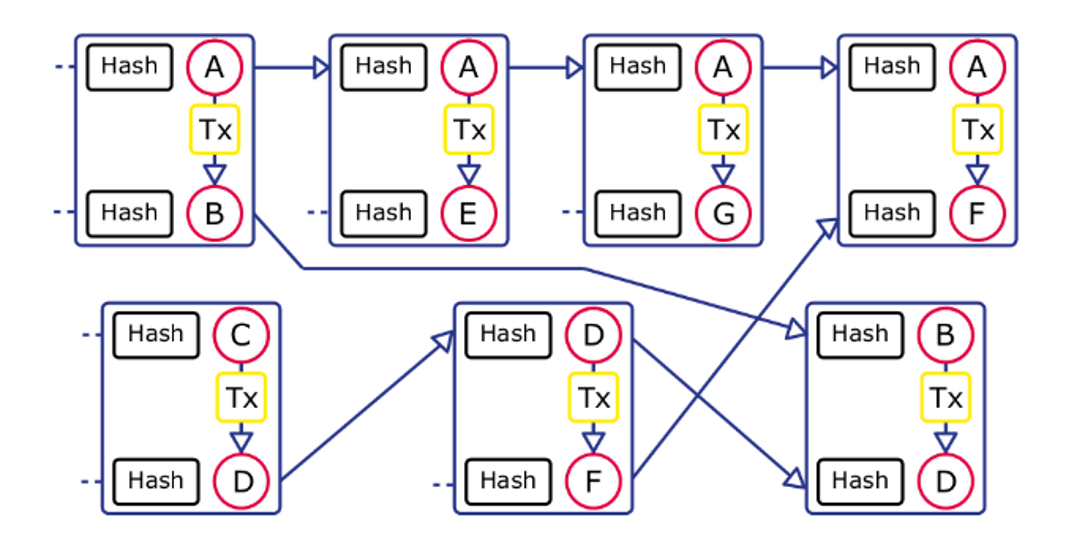
\includegraphics[scale=0.5]{Trustchain.png}
\caption{TrustChains of different network participants (taken from \cite{TrustChain: A Sybil-resistant scalable blockchain}).}
\label{fig:Trustchain}
\end{center}
\end{figure} 

\noindent{}This structure is strongly scalable, both in the number of agents in the network as well as in the number of transactions per agent as TrustChain does not maintain a global consensus. This means that double-spend attacks are not actually prevented, as they are in traditional blockchains. However, they are made detectable through a gossip-protocol, as peers share information about other nodes' transaction histories and can subsequently be penalised. Thereby fraudulent activity is not actually prevented, but strongly disincentivised.\vspace{1em}\\


\newpage
\chapter{Research Question}
\label{chap:Research Question}
\noindent{}The Tribler P2P network aims to incorporate a reputation mechanism into their application to enforce indirect reciprocity and thereby achieve cooperation. Ultimately, the goal is to determine an algorithm that takes the TrustChains of agents participating in the network and returns some reputation scores for these nodes. Reputation is subjective and therefore reputations should be determined by all nodes independently based on the data they have gathered through the gossip protocol. There are many algorithms that spring to mind that may achieve a desirable outcome in this setting. However, designing such an algorithm comes with a particular set of challenges that must be overcome for it to be effective. This leads us to our research question:

\begin{center}
\noindent{}{\it What requirements does a reputation mechanism need to satisfy to induce cooperative behaviour in a P2P file sharing network?} \vspace{1em}\\
\end{center}
 
\noindent{}In order to answer this question we begin by refining our understanding of a reputation mechanism. In \cite{On the Sybil-Proofness of Accounting Mechanisms} Seuken \& Parkes (2011) introduce the concept of {\it accounting mechanisms} which are mappings on a social interaction graph representing the reputability that agents in the P2P network have based on their interaction histories. If one agent is assigned a higher score than another agent by this mapping then that agent is considered more reputable. The main idea is that a sensible accounting mechanism should assign higher scores to nodes who make overall larger contributions to the network and consume less than other nodes. A node with a higher reputation score should then find itself more likely to be served data, therefore stimulating cooperative behaviour. Conversely, agents that behave selfishly should be assigned lower reputation scores and should therefore be less likely to receive data, disincentivising selfish behaviour. \vspace{1em}\\

\noindent{}Ideally, accounting mechanisms should entail some transitivity, by which we mean nodes assign agents that they have had direct interactions with higher reputation scores than nodes they have not had direct interactions with. The larger the distance between two nodes in the social interaction graph the smaller the reputational reward for a contribution. Additionally, contributions that are indirect contributions to a node should lead to higher reputation scores than contributions that are not indirectly benefitting this node. By indirect contributions we mean that if a node contributes some resources to another node which in turn serves a third node, then the third node will consider the contributions made by the first node indirect contributions to itself. This would accurately capture the concept of reputation as encountered in the real world. \vspace{1em}\\ 

\noindent{}Lastly, an accounting mechanism should successfully prevent \textbf{lazy freeriding}. We consider an agent that consumes far more resources than they contribute a lazy freerider. More rigorously, we say that if the net contributions a node has made to the rest of the network, i.e. the amount they have consumed subtracted from the amount they have contributed, exceed a certain lower bound then that node is a lazy freerider. Alternatively, we might say that if the ratio of these values exceeds a given lower bound then that node is a lazy freerider. An accounting mechanism should penalise excessive leeching in a manner that makes it impossible for a node to go below such a threshold.\vspace{1em}\\

\noindent{}So far, this question seems like a rather easy one to solve. There are plenty of algorithms that will capture these requirements and prevent lazy freeriding. However, the question is complicated by the possibility of attacks on the file sharing network. In this work we will focus on two types of attacks in particular, namely misreport attacks and sybil attacks. \vspace{1em}\\


\noindent{}A {\bf misreport attack} is performed by one or more malicious agents who do not report honestly on their own past interactions. Malicious agents may try to deceive honest agents by reporting on transactions that have not actually occurred or by concealing transactions  that may reduce their standing in the network. By this method agents can increase their reputation or reduce the standing of other nodes in the network. In \cite{Accounting Mechanisms for Distributed Work Systems} Seuken \& Parkes (2011) have introduced a mechanism which solves this problem to some degree. In this work we examine the ability of the TrustChain architecture to prevent this type of attack. \vspace{1em}\\ 

\noindent{}A {\bf sybil attack} occurs when a single malicious agent creates multiple, often times large amounts of, fake identities. This agent will then attempt to exploit the control they have over the accounts in order to artificially increase the reputation score of one or more of their identities by reporting high levels of reputability through fake transactions without actually performing any work. Another approach may be to simply reduce the reputation of other honest nodes in the network to improve their own relative standing(s). This can be done because Sybil identities can create forged reports about one another. Such attacks can have strongly detrimental effects on the functioning of P2P networks, especially if carried out on a large scale. If the creation of identities and forging of transactions are cheap compared to their gain, then such attacks have the potential to disrupt entire file-sharing networks.  \vspace{1em}\\

\noindent{}Given these types of attacks we can narrow down our research question to the following
\begin{center}
{\it What requirements does an accounting mechanism need to satisfy in order to effectively incentivise cooperation and prevent lazy freeriding, while being resistant to misreport attacks and mitigating the effects of sybil attacks?}
\end{center}

\begin{comment}
\subsection{Other Types of Attacks}
\label{subsec:Other Types of Attacks}
\noindent{}There are many other types of attacks one can perform to disrupt p2p networks and we will not be able to analyse the effects of all of these in this thesis. Some of the more prominent attacks are mentioned below. Note however, that the main focus of our thesis will, from here on out, lie on preventing lazy freeriding and mitigating sybil attacks. \vspace{1em}\\

\subsubsection{Collusion Attacks}
\label{subsubsec:Collusion Attacks}
\noindent{}Collusion attacks resemble sybil attacks in that a group of nodes cooperate in an attempt to behave maliciously without being punished or detected. The difference between these types of attacks and sybil attacks lies in the fact that the colluding agents are controlled by different parties and may be far away from each other, geographically. In a sybil attack the nodes that collude are controlled by one and the same party. An example of a collusion attack my be given by several nodes getting together and reporting positive transactions about one of their members $j$ to an honest node $i$. This increases the chances of $j$ being served some data by $i$, which it may then, in turn, distribute to other participants of the collusion attack. This type of attack is very difficult to prevent as there may not be any noticeable sign of it in the work graph. Luckily these types of attack are quite rare and usually not that beneficial as there is an inherent problem of trust among the malicious nodes.\vspace{1em}\\

\subsubsection{Eclipse Attacks}
\label{subsubsec:Eclipse Attacks}
\noindent{}An eclipse attack lies halfway between a sybil attack and a misreport attack. A malicous agent $j$ may choose to impersonate multiple identities in the network in an attempt to shield an innocent node from the rest of the network. The goal is to prevent the attacked node from obtaining reports about certain transactions in the network and therefore to isolate it in a part of the network that is predominantly malicious and controlled by the attacker. \vspace{1em}\\

\subsubsection{Malware Distribution \& and DDoS Attacks}
\label{subsubsec:Malware Distribution & and DDoS Attacks}
\noindent{}Another way of attacking the network is by injecting useless data and/or even malware into the network, thereby "poisoning" the traffic. The intent may either be to directly attack individual peers by providing them with camouflaged corrupted files, or to simply choke of network traffic. This can be done by inserting fake records into the index pointing to a target IP and port number. When an agent then looks up a file it will receive fake location information from a poisoned index. This can slow the network traffic to a crawl. \vspace{1em}\\

\subsubsection{Whitewashing Attacks}
\label{subsubsec:Whitewashing Attacks}
\noindent{}Lastly, a whitewashing attack occurs when an agent deletes their identity from the network and starts from scratch with a new identity. This way an agent can whitewash their history in the network. This is done to evade negative repercussions of malicious behaviour and start afresh as a newcomer node. An example for this may be an agent in a social media network that has been exposed as distributing malignant content, closing and reopening a new account, only to resume the same strategy.\vspace{1em}\\  
\end{comment}


\begin{comment}
\section{Related Work}
\label{sec:Related Work}
\noindent{}The body of literature researching reputation mechanisms on social interaction graphs is quite large and we have limited our scope, for the most part, to the research conducted by authors Seuken and Parkes, who have made large contributions to the research of this exact question. The research that we focused on the most throughout this thesis is their paper titled "On the Sybil-Proofness of Accounting Mechanisms", in which they discuss some impossibility results for the prevention of sybil attacks \cite{On the Sybil-Proofness of Accounting Mechanisms}. They define 3 requirements accounting mechanisms must satisfy in order for them \textbf{not} to be sybil resistant. Later they relax their definition of sybil-proofness to only include up to $K$ sybil identities and introduce two additional restrictions for accounting mechanisms to satisfy this definition of sybil resistance. We will critically examine these results and expand on their research. \vspace{1em}\\

\noindent{}The same authors have produced a variety of results to ensure the resistance of accounting mechanisms against misreport attacks and sybil attacks. Their most notable mechanism against misreports is called DropEdge defined in \cite{Accounting Mechanisms for Distributed Work Systems} and expanded in \cite{Sybil-proof Accounting Mechanisms with Transitive Trust}, which we will reintroduce in this thesis and compare to Tribler's TrustChain architecture \cite{TrustChain: A Sybil-resistant scalable blockchain}. \vspace{1em}\\

\noindent{}They have also evaluated a number of different graph theoretical centrality measures in their applicability in this problem, such as the PageRank algorithm, a maximum-flow based centrality measure called BarterCast as well as a hitting time algorithm. They analysed their resistance to sybil attacks by various metrics such as rank-strategyproofness, value-strategyproofness and upwards value-proofness as well as relaxed versions of these metrics \cite{Hybrid Transitive Trust Mechanisms}. Other metrics for the evaluation of accounting mechanisms are informativeness, misreport-proofness and long-term misreport-proofness \cite{Sybil-resistant Trust Mechanisms in Distributed Systems}. \vspace{1em}\\ 

\noindent{}They discuss some more properties of accounting mechanisms, such as work-monotonic transitive trust and strong transitive trust, narrowing down the definition. Lastly, they invent the concept of hybrid transitive trust mechanisms, which are the convex combination of accounting mechanisms. These may satisfy nice properties than "single" accounting mechanisms as they may combine nice properties of several accounting mechanisms \cite{Hybrid Transitive Trust Mechanisms}.\vspace{1em}\\

\noindent{}Another very relevant piece of work is Otte's "Sybil-resistant trust mechanisms in distributed systems", in which a completely new accounting mechanism, called netflow, is introduced. The authors evaluate this mechanism based on the metrics given above. The authors show that this mechanism satisfies sybil-resistant according to the definition given by the authors above. Lastly, they also examine the temporal pagerank algorithm as a possible accounting mechanism and its resistance to sybil attacks under a given time restriction.\vspace{1em}\\  
\end{comment}

\begin{comment}
\item[Sybil-proof Accounting Mechanisms with Transitive Trust:] They introduce the concept of strong transitive trust (think through and explain nicely later). They also introduce the concept of long-term misreport-proofness, which include dynamic graphs (i think...). They claim that dropedge is long-term misreport-proof. They refine the concept of weakly beneficial sybil attacks, but still keep the ambiguity in it. They state a new impossibility theorem. Then introduce weak transitive trust and a new variant of drop-edge and claim that the two will still yield weakly beneficial sybil attacks. They then show that their theorem is "tight", which means that if any of the things dicussed above are not satisfied anymore the assertion no longer holds.
\item[Hybrid Transitive Trust Mechanisms:] They work on the trust graph and introduce the definition of transitive trust mechanisms (here they rewrite their accounting mechanism the way we did). Here they finally define misreport!!! Quite similar to us, except they have culprite while we don't. They introduce rank-strategyproofness and value-strategyproofness. Examples of transitive trust mechanisms PGR, Hitting Time, MaxFlow, ShortesPaths then they explain whether these are rank-and value-strategyproof. They come up with hybrid mechanisms, where you take two mechanisms and take convex combo of them. Then they have theorems about value-and rank-strategyproofness of hybrid mechanisms. They relax their notions of these things to eps-rank(values) strategyproof and make statements of about hybrid mechanism strategyproofness. They have some examples of which mechanisms satisfy this. They relax value-strategyproofness to upwards value-proofness and extend their results. 
\item[Otte:] Introduce interaction model, which we will disagree with as it doesn't have possibility for misreports. Very nice for TrustChain though. Make the same mistake with sybil attack profit. Come up with their own accounting mechanism called Netflow limited contribution. Then they show that it is resistant to weakly beneficial sybil attacks. They introduce definition of informativeness.. it's not so informative, so they scale it to be more informative. They discuss some weaknesses of netflow and its resistance to other attacks. They then discuss temporal pagerank and simulate it... 
\end{comment}


\section{Thesis Summary and Contributions}
\label{sec:Thesis Summary and Contributions}
\noindent{}In chapter \ref{chap:Mathematical Framework for Accounting Mechanisms} we begin by mathematising the relevant concepts such as transactions, work graphs, accounting mechanisms, allocation policies, lazy freeriding, misreports, sybil attacks and the TrustChain architecture. We prove the resistance of accounting mechanisms that are based on the TrustChain architecture to misreports under some mild restrictions and we prove the resistance of certain types of accounting mechanisms to lazy freeriding. This chapter is meant to simply provide a framework in which we can conduct our research. \vspace{1em}\\

\noindent{}In chapter \ref{chap:Sybil Attack Gain} we elaborate on the effects of sybil attacks. We introduce the concept of its cost and profit for the attacker. The cost of a sybil attack turns out to be easily explained, while defining the profit turns out to be more involved. We solve this problem by postulating an interaction model in which we also evaluate which allocation policies are most resistant to sybil attacks. Given this model we can determine a formula for the profit of a sybil attack. This is the amount of additional work that can be consumed by the attacker after the attack has been carried out. Seeing as this formula is based on a discrete stochastic process we realise that it is impossible to compute in a generic setting. In order to obtain values for the cost and profit of a sybil attack that are practically computable we redefine these values for accounting values, i.e. the aggregate of additional accounting values obtained by the attacker and its sybils. We believe that rigorous definitions of these terms are much needed and have been neglected in the existing literature such as in \cite{On the Sybil-Proofness of Accounting Mechanisms}. \vspace{1em}\\

\noindent{}The values of sybil attack cost and profit in terms of accounting values are now much easier to compute. However, they are not actually the relevant metric, but just a proxy for the earlier defined cost and profit of sybil attacks in terms of work. Given these two different definitions we investigate the relationship between them. We introduce examples where the two above are not equivalent in chapter \ref{chap:Representativeness of Accounting Mechanisms}. This turns out to be very problematic indeed as accounting mechanisms only serve as a representation of a node's cooperativeness and a sybil attacker aims to increase these in an attempt to obtain more work from the network. Therefore we find that some accounting mechanisms do not allow for accurate assessment of sybil attack profit. In order to circumvent this dilemma we come up with the definition of representativeness to ensure consistency between these two concepts of sybil attack profit.\vspace{1em}\\

\noindent{}In chapter \ref{chap:On the Impossibility of Sybil-Proofness} we analyse existing impossibility results from the literature which state under which conditions accounting mechanisms are susceptible to sybil attacks that enable the attackers to consume large amounts of data \cite{On the Sybil-Proofness of Accounting Mechanisms}. We detect an error in an important theorem and extend the existing model to circumvent this error. We introduce two additional properties of accounting mechanisms which ensure the existence of impactful sybil attacks and produce two further impossibility results as well as consequent corollaries for slightly relaxed versions of the two properties.\vspace{1em}\\

\noindent{}In our last chapter, chapter \ref{chap:Sybil-Proofness of Accounting Mechanisms} we aim to do the inverse of what we did in chapter \ref{chap:On the Impossibility of Sybil-Proofness}, i.e. introduce properties for accounting mechanisms to be resistant to strongly beneficial sybil attacks. We begin by characterising certain types of passive sybil attacks, namely parallel and serial attacks. Next, we introduce requirements for accounting mechanisms to be resistant to these types of attacks. We extend the model to a particular type of sybil attack to which accounting mechanisms that are resistant to the upper types of attacks, are also resistant. Lastly, we extend our requirements for accounting mechanisms by an aditional property to be obtain resistance to arbitrary types of sybil attacks as well. \vspace{1em}\\

\noindent{}In the appendix in chapter \ref{chap:Appendix} we address research we conducted that did not turn out to be fruitful. The first approach to solving this problem was through a model based on geographic proximity of participants in the network. The second topic we analysed was the topic of the evolution of cooperation among biological organisms. For this we made a month long research visit to Japan to analyse properties reputation mechanisms should satisfy to be able to facilitate cooperative behaviour. \vspace{1em}\\

\begin{comment}
\begin{itemize}
\item We critically evaluate existing literature, especially Seuken \& Parkes impossibility results (found mistakes)
\item We introduce much needed definition of sybil attack cost profit (lead to error in impossibility results)
\item We introduce additional constraints for accounting mechanism impossibility results
\item We introduce definition of representativeness to fix incongruence of attack cost and profit
\item We characterise sybil attacks and introduce requirements for accounting mechanisms to be sybil resistant
\end{itemize}
\end{comment}

\chapter{Mathematical Framework for Accounting Mechanisms}
\label{chap:Mathematical Framework for Accounting Mechanisms}
\noindent{}We begin by introducing a mathematical framework for the setting in which we conduct our research, namely by rigorously formalising interactions (transactions) between nodes in the network. In \cite{Sybil-resistant Trust Mechanisms in Distributed Systems} Otte et al. (2016) introduced the concept of an {\it ordered interaction model} from which an {\it ordered interaction graph} and a {\it block graph} are derived. While this is a very elegant definition for a set of transactions and the derivation of a work graph from it, it is directly tailored to the TrustChain architecture and lacks the possibility of misreports and counterfeit interactions. Therefore we will not adopt it here, but instead derive a slightly different and more generic definition of a transaction set, which will be our equivalent to their ordered interaction model.\vspace{1em}\\


\section{Network Transactions}
\label{sec:Network Transactions}
\noindent{}We start off with the definition of a simple network transaction, or interaction, which simply denotes the transference of data in between two nodes.\vspace{1em}\\

\begin{definition}[Agent Transaction]\ \\
\label{def:Agent Transaction}
\noindent{}Let $V$ be the set of all agents in the network and let $pr_1,pr_2,pr_3$ denote the canonical projections on the cartesian product of 3 sets. A transaction $t\in{}V^2\times\mathbb{R}_{>0}$ between two nodes $i,j\in{}V$ is given by a tuple $(i,j,w)$, whereby $pr_1(t)$ is the contributer and $pr_2(t)$ is the recipient of the work performed. $w$ or $pr_3(t)$ corresponds to the size of the transaction, i.e. the amount of data transferred from $pr_1(t)$ to $pr_2(t)$. \vspace{1em}\\ %Finally, $id\in\mathbb{R}$ is the unique transaction identifier.
\end{definition}

\noindent{}Note that for any transaction $t$ it must always hold $pr_1(t)\neq{}pr_2(t)$, i.e. nodes cannot transact with themselves. Secondly, transactions are unidirectional. This means that a single transaction cannot contain the transference of data from node $i$ to node $j$ {\bf and} vice versa. Hence, the ordering of the two nodes in the transaction tuple is not arbitrary, but determined by which of the two is making the contribution and who is receiving it. Lastly, it naturally always holds that $w\geq{}0$. \\

\noindent{}As every node participates in a string of transactions in a given chronological order, we obtain a series of transactions for every node $i$, which we will refer to as a transaction sequence.\vspace{1em}\\

\begin{definition}[Transaction Sequence]\ \\
\label{def:Transaction Sequence}
\noindent{}The transaction sequence of a node $i\in{}V$ is expressed as $TS_i:=(t_{i,n})_{n\in\mathbb{N}_{\leq{}T_i}}$ where $t_{i,n}$ is the $n$-th transaction node $i$ participated in, either as a contributor or as a consumer. As above $t_{i,n}$ is given by a tuple $(j,k,w)$ where either $j=i$ or $k=i$. $T_i$ denotes the length of $i$'s transaction sequence, i.e. the number of transactions $i$ has participated in thus far. It grows as time progresses.\vspace{1em}\\
\end{definition}

\noindent{}Note that in this definition we implicitly assume that concurrent transactions can be deterministically serialised. Else, the ordering of transactions would become nonsensical. As time goes on, transaction sequences obtain new entries and continue to grow, which implies that $T_i$ is not a static value, but changes over time. We choose not to incorporate a temporal variable in this model and instead assume that a transaction sequence represents a "snapshot in time" as opposed to a dynamic variable. Next, we define a transaction function, which will denote the size of a transaction.\vspace{1em}\\

\begin{definition}[Transaction Function]\ \\
\label{def:Transaction Function}
\noindent{}For every node $i\in{}V$ we define a transaction function $t_i$, given by 
\[
t_i:\mathbb{N}_{\leq{}T_i}\times{}V\rightarrow{}\mathbb{R},
\]
\noindent{}where $t_i(m,j)$ corresponds to the amount of work node $i$ has leeched from or contributed to node $j$ in its $m$-th transaction, i.e. 
\[
t_i(m,j) = \left\lbrace 
\begin{array}{lll}
pr_3(t_{i,m}), & \textrm{if} & pr_2(t_{i,m})=j \\
-pr_3(t_{i,m}), & \textrm{if} & pr_1(t_{i,m})=j \\
0, & \multicolumn{2}{l}{\textrm{otherwise}} \\
\end{array}.
\right.
\]
\end{definition}
\noindent{}Note that it holds 
\[
t_i(m,j)>0\,\,\,\,\textrm{if } pr_1(t_{i,m})=i
\]
\noindent{}and 
\[
t_i(m,j)<0\,\,\,\,\textrm{if } pr_2(t_{i,m})=i.
\]
\noindent{}It is obvious that the two conditions above can never both be satisfied simultaneously. This is due to our restriction made in definition \ref{def:Agent Transaction}, where we stated that for any transaction $t$ it must always hold $pr_1(t)\neq{}pr_2(t).$\vspace{1em}\\ 


\begin{remark}[Symmetry of Transaction Functions]\ \\
\label{rem:Symmetry of Transaction Functions}
\noindent{}In theory it should always hold for any pair of nodes $i,j\in{}V$ and any value $w\neq{}0$  
\[
\left|\left\lbrace{}n\in\mathbb{N}_{\leq{}T_i}\,|\,t_i(n,j)=w\right\rbrace\right| = \left|\left\lbrace{}m\in\mathbb{N}_{\leq{}T_j}\,|\,t_j(m,i)=-w\right\rbrace\right|.\vspace{1em}\\
\]

%\[
%\forall{}i,j\in{}V,n\in\mathbb{N},\,t_i(n,j)=w\neq{}0:\exists{}m\in\mathbb{N},\,t_j(m,i)=-w
%\]

\noindent{}What this means is that any transaction between nodes $i$ and $j$ that is contained in the transaction sequence of $i$ must also be contained in the transaction sequence of node $j$. This is quite trivially true if the transaction sequences of both parties contain all transactions that they have participated in. We call this property {\it symmetry of transaction functions}.\vspace{1em}\\
\end{remark}

\noindent{}Finally, we introduce the set containing all transactions that have transpired in the network, denoted by 
\[
TS:=\left\lbrace{}TS_i\,|\,i\in{}V\right\rbrace .
\]

\noindent{}This set contains all transaction sequences of all nodes in the network. Based on our remark \ref{rem:Symmetry of Transaction Functions} we see that $TS$ must contain every transaction exactly twice.\vspace{1em}\\

\noindent{}Recall that in a distributed system there is no central authority and therefore no central database keeping record of all transaction sequences. Hence, an agent can only know their own transaction sequence and those of agents who've shared their transaction sequences with them. Agents are unlikely to be aware of the transaction sequences of all agents in the network, or of who is in the in the network in the first place. Hence no agent can know the transaction set $TS$. \vspace{1em}\\

\noindent{}Agents query one another's transaction sequences which are then shared and disseminated along the network. In \cite{Creating Trust through Verification of Interaction Records} Harms et al. (2018) propose a record dissemination protocol, which is based on the TrustChain architecture, discussed in section \ref{sec:Blockchains & TrustChain}. We will not delve into the details of mechanisms facilitating this distribution of transaction sequences, but will simply assume that there is one in place and continue. \vspace{1em}\\

\begin{definition}[Agent Information]\ \\
\label{def:Agent Information}
Let $i\in{}V$ be an arbitrary, but fixed agent in the network. An interaction $(j,k,w)$ between two agents $j,k\in{}V$, that $i$ receives a report about from $j$ is written as $t_{j,m}^i$, where the $m$ means that it's the $m$-th transaction in the transaction sequence $j$ has shared with $i$. The transaction sequence $j$ reports to $i$ is then denoted by $TS_j^i:=(t_{j,m}^i)_{m\leq{}T_j^i}$. Here $T_j^i$ is the length of $TS_j^i$. We derive the transaction function of $j$ that $i$ has information on as 
\[
t_j^i(m,k)=\left\lbrace 
\begin{array}{lll}
pr_3(t_{j,m}^i), & \textrm{if} & pr_2(t_{j,m}^i)=k \\
-pr_3(t_{j,m}^i), & \textrm{if} & pr_1(t_{j,m}^i)=k \\
0, & \multicolumn{2}{l}{\textrm{otherwise}} \\
\end{array}.
\right. \vspace{1em}\\
\]
\noindent{}When aggregated into a set of all transaction sequences, $i$ obtains the {\it subjective} transaction set 
\[
TS^i:=\left\lbrace{}TS_j^i\,|\,j\in{}V\right\rbrace.
\]
\noindent{}Recall that $TS$ contained every transaction exactly twice. This is no longer true for $TS^i$ as different agents may report transaction sequences inconsistently. This means agent information may be contradictory or flawed. \vspace{1em}\\
\end{definition}

\noindent{}So far, we have not ensured that agents sharing their transaction sequences will do so honestly and consistently. Agents may choose to add transactions that haven't occurred to their transaction sequence or drop transactions from their sequence. Agents may even refuse to share their transaction history entirely. This type of behaviour is what we defined earlier as {\it misreports}, which we will define more rigorously now. \vspace{1em}\\

\begin{definition}[Misreport Attack]\ \\
\label{def:Misreport Attack}
Let $i\in{}V$ be an arbitrary but fixed agent with subjective transaction set $TS^i$. We say that a misreport between two agents $j,k\in{}V$ has occurred if there exists a $w\neq{}0$ such that 

\[
\left|\left\lbrace{}n\in\mathbb{N}_{\leq{}T_j^i}\,|\,t_j^i(n,k)=w\right\rbrace\right| \neq \left|\left\lbrace{}m\in\mathbb{N}_{\leq{}T_k^i}\,|\,t_k^i(m,j)=-w\right\rbrace\right|.
\]
\end{definition} 

\noindent{}Put in words this simply means that a misreport between two agents $j$ and $k$ has occurred if there exists an agent $i$ who receives reported transaction sequences $TS_j^i$ and $TS_k^i$ such that the there exists a transaction between $j$ and $k$, which is contained in the reported transaction sequence of one of the two, but not in both. \vspace{1em}\\

\noindent{}Note that we say a misreport {\it has occurred} instead of a misreport was {\it committed by} as it is not clear to agent $i$ which of the two agents $j$ and $k$ is responsible for the misreport. If a transaction is contained in the reported transaction sequence of agent $k$ and not in that of $j$, then either $k$ may have fabricated a transaction or $j$ may have dropped a transaction from their sequence. From the perspective of $i$ these two cases are indistinguishable.\vspace{1em}\\

\section{Work Graphs}
\label{sec:Work Graphs}
\noindent{}Given the set of all transactions $TS$, one can transform the transaction sequences into a {\it work graph} with the help of a mapping function. A work graph is a directed network graph visualising the interactions between nodes. It may be unidirectional or even a double-edged graph. The idea is that edges between vertices correspond to overall seed-leech relationships of nodes in the network. \vspace{1em}\\

\begin{definition}[Work Graph]\ \\
\label{def:Work Graph}
\noindent{}A work graph is given by the tuple $G = (V, E, w)$, whereby $V$ is the set of vertices, i.e. agents in the network and $E$ is a set of directed edges between the agents. An edge $(i,j)\in{}E$ pointing from node $i$ to node $j$ represents node $j$ performing work for node $i$. \vspace{1em}\\ The function $w:V\times{}V\rightarrow{}\mathbb{R}_{\geq{}0}$ denotes the weight of the edges, i.e. $w(i,j)$ represents the total amount of work performed by node $j$ for node $i$. If two nodes $i$ and $j$ are not connected then we set the edge weights $w(i,j)=w(j,i)=0$. We choose the set of edges $E\subset{}V\times{}V$ such that $(i,j)\in{}E$ if and only if $w(i,j)>0$. Note that it must always hold $w(i,i)=0$ f.a. $i\in{}V$ as we do not allow for agents to transact with themselves.\vspace{1em}\\ 
\end{definition}

\noindent{}There are a number of different ways transactions in $TS$ can be aggregated to form edges in the work graph. In the {\it unidirectional, single-edge} case of the work graph the edges of the graph can be derived from the set of transaction functions by
\[
w(i,j) = \max\left\lbrace{}\sum\limits_{n\in\mathbb{N}_{\leq{}T_j}}t_j(n,i), 0\right\rbrace = \max\left\lbrace{}-\sum\limits_{n\in\mathbb{N}_{\leq{}T_i}}t_i(n,j), 0\right\rbrace
\]
and conversely, 
\[
w(j,i) = \max\left\lbrace{}\sum\limits_{n\in\mathbb{N}_{\leq{}T_i}}t_i(n,j), 0\right\rbrace = \max\left\lbrace{}-\sum\limits_{n\in\mathbb{N}_{\leq{}T_j}}t_j(n,i), 0\right\rbrace.
\]

\noindent{}Here the weight of the edges corresponds to the net data flow in between two nodes. The edge is directed toward the node that has a positive deficit in the bilateral relationship. Note that there can only be a single edge connecting two nodes, which points from one to the other, i.e. for any pair of nodes $i,j\in{}V$ it holds $w(i,j)>0\,\,\Rightarrow\,\,w(j,i)=0$. This type of work graph is quite useful as it nicely captures the overall net contributions nodes have made to the network. Another advantage this type of work graphs has is its simplicity as there is never more than one edge connecting two nodes. \vspace{1em}\\

\noindent{}Note that there is one drawback to this approach, which lies in the fact that the single-edge graph neglects certain contributions made to the network. For instance, if two agents have donated the same amount of resources to one another then the weight of the edge connecting them is zero. Hence, this type of graph lacks informativeness as it only captures net contributions.\vspace{1em}\\

\noindent{}An alternative to this are double-edged graphs in which case, we can derive the edge weights as follows
\[
w(i,j) = \sum\limits_{n\in\mathbb{N}_{\leq{}T_j}}\max\left\lbrace{}t_j(n,i), 0 \right\rbrace = \sum\limits_{n\in\mathbb{N}_{\leq{}T_i}}\max\left\lbrace{}-t_i(n,j),0\right\rbrace 
\]
\noindent{}and
\[
w(j,i) = \sum\limits_{n\in\mathbb{N}_{\leq{}T_i}}\max\left\lbrace{}t_i(n,j), 0 \right\rbrace = \sum\limits_{n\in\mathbb{N}_{\leq{}T_j}}\max\left\lbrace{}-t_j(n,i),0\right\rbrace.
\]

\noindent{}In this particular type of graph an edge $(i,j)$ corresponds to the gross data flow from $j$ to $i$ without subtracting the work $i$ has done for $j$. A positive attribute of this this type of graph is that it's generally more informative as it doesn't reduce edge weights to net data flow. Throughout this thesis we will always assume a double-edged work graph.\vspace{1em}\\

\noindent{}Given a transaction set $TS$, we can derive this type of work graph using the mapping function mentioned above. We write $G=g(TS)$ where $g$ maps the transaction set $TS$ to the work graph $G$, according to the classifications above. \vspace{1em}\\

\noindent{}It may be somewhat counterintuitive for edges to be pointing from the recipient to the contributor. Note that we can invert the edges as well, such that an edge $(i,j)$ pointing from $i$ to $j$ corresponds to work performed by $i$ for $j$, in that case we obtain. 
\[
w(i,j) = \sum\limits_{n\in\mathbb{N}_{\leq{}T_i}}\max\left\lbrace{}t_i(n,j), 0 \right\rbrace = \sum\limits_{n\in\mathbb{N}_{\leq{}T_j}}\max\left\lbrace{}-t_j(n,i),0\right\rbrace.
\]

\noindent{}However, we choose to stick with the former direction with a particular set of accounting mechanisms in mind. Although, this is quite irrelevant. For an example of how to derive a work graph from a transaction set see the example below.\vspace{1em}\\

\begin{example}[]\ \\
\label{ex:Example Transaction Set and Work Graph}
\noindent{}Take the tabular below as the transaction sequences of 4 agents $i,j,k,h\in{}V$. Then the mapping function $g$ returns the corresponding work graph $G$ with directed double-edges derived from the transaction set $TS$ as seen in figure 3.1. \vspace{1em}\\

\begin{comment}


\begin{tabular}{c|c|c|c}
$i$ & $k$ & $j$ & $h$ \\
\hline
$(i,j,3)$ & $(k,j,2)$ & $(j,h,4)$ & $(h,i,9)$ \\
$(h,i,9)$ & $(i,k,2)$ & $(j,i,1)$ & $(j,h,4)$ \\
$(j,i,1)$ &           & $(i,j,3)$ &           \\  
$(i,k,2)$ & 		  & $(k,j,2)$ & 
\end{tabular}
\end{example}


\end{comment}

\begin{figure}[H]
\includegraphics[scale=0.6]{"Example Objective Work Graph".PNG}
\label{fig:Example Work Graph}
\caption{Example Work Graph}
\end{figure}
\end{example}


\begin{remark}[]\ \\
\label{rem:P2P, Twitter, Facebook}
\noindent{}Note that in our case we introduce the work graph with regard to peer-to-peer filesharing, keeping the application of the {\it Tribler} network in mind \cite{Tribler}. This means that the work performed, i.e. the weight of the edges, corresponds to the amount of data transferred from one node to another, by seeding and leeching respectively. \vspace{1em}\\

\noindent{}However, with our examples of social networks, such as Facebook and Twitter from chapter \ref{chap:Introduction} in mind, we would like to extend our model to entail these networks and any kind of P2P network in general. In the case of these social networks we can apply the exact same concepts, but reinterpret the transactions between agents as "follow" or "friendship" relations, etc. The weights of these edges could then, for instance, be determined by the number of likes and/or retweets a user receives from a follower/friend. \vspace{1em}\\
\end{remark}

\begin{example}[]\ \\
\label{ex:Example Graphs (P2P, Twitter, Facebook)}
In the case of {\it Facebook} a friendship may correspond to an undirected edge connecting two vertices, while the amount of likes and/or mentions these people receive from one another, could be represented by another pair of edges connecting the two. An example of such a work graph is given in figure \ref{fig:Facebook Example Graph} below.

\begin{figure}[H]
\begin{center}
\includegraphics[scale=0.9]{"Facebook Example Graph".PNG}
\caption{Facebook Example Graph}
\label{fig:Facebook Example Graph}
\end{center}
\end{figure}

\noindent{}A follower relationship on {\it Twitter} could be represented by an edge pointing from the follower to the followed, while the edge weight may correspond to the number of tweets that have been liked or retweeted, etc. In this particular application a bidirectional graph will be more reasonable than a unidrectional one, as can be seen in figure \ref{fig:Twitter Example Graph} below.
\begin{figure}[H]
\begin{center}
\includegraphics[scale=0.8]{"Twitter Example Graph".PNG}
\caption{Twitter Example Graph}
\label{fig:Twitter Example Graph}
\end{center}
\end{figure}
 
\end{example}

\noindent{}Recall the fact that agents in the network were not aware of all transactions that have occurred and definition \ref{def:Agent Information}, in which we stated that agents build a subjective transaction set based on agent reports. It follows from this that the work graph defined above is unlikely to be known by any node in the network. Instead, agents build, what is referred to, as a subjective work graph from their subjective transaction sets. This follows the same paradigm as above with one difference, which arises due to the possibility of misreporting. \vspace{1em}\\

\noindent{}As mentioned in definition \ref{def:Misreport Attack} agents may report contradictory transaction sequences. This results in a work graph with edge weights given by tuples in $\mathbb{R}_{\geq{}0}\times\mathbb{R}_{\geq{}0}$, whereby one entry of the tuple corresponds to the aggregated data flow between the two nodes, as reported by one of them, while the other corresponds to the same value, but reported by the other. \vspace{1em}\\

\begin{definition}[Subjective Work Graph]\ \\
\label{def:Subjective Work Graph}
\noindent{}A subjective work graph from the perspective of node $i$ is given by a tuple $G_i=(V_i,E_i,w_i)$ where $V_i\subset{}V$ and $E_i\subset{}V_i\times{}V_i$. As in the definition of the work graph an edge $(j,k)\in{}E_i$ pointing from $j$ to $k$ represents work performed for $j$ by $k$.\vspace{1em}\\

\noindent{}For two nodes $j,k\in{}V_i$ the value $w_i(j,k)$ denotes the weight of the edge connecting $j$ and $k$, as reported by both nodes in question to node $i$. Seeing as two nodes may report different transaction sequences, $w_i(j,k)$ is determined by a tuple $w_i(j,k) = (w_j^i(j,k), w_k^i(j,k))$. As before, if two nodes are not connected (from the perspective of $i$), we set $w^i(j,k)=0=w^i(k,j)$ and we choose the set of edges $E_i$ such that $(j,k)\in{}E_i$ if and only if either $w_j^i(j,k)>0$ or $w_k^i(j,k)>0$. As in definition \ref{def:Work Graph}, we do not allow edges $w_i(j,j)$ for any $j\in{}V_i$.
\end{definition}

\noindent{}The transaction sequences in $TS_i$ can be aggregated into edge weights analogously to our earlier definition of the work graph (\ref{def:Work Graph}). In the {\it unidrectional, single-edge} case the edge weights of the subjective work graph $G_i$ are determined by 

\[
w^i(j,k)=\left( \max\left\lbrace{}\sum\limits_{n\in\mathbb{N}_{\leq{}T_k^i}}t_k^i(n,j), 0\right\rbrace, \max\left\lbrace{}-\sum\limits_{n\in\mathbb{N}_{\leq{}T_j^i}}t_j^i(n,k), 0\right\rbrace \right)
\]
\noindent{}and consequently
\[
w^i(k,j) = \left(\max\left\lbrace{}\sum\limits_{n\in\mathbb{N}_{\leq{}T_j^i}}t_j^i(n,k), 0\right\rbrace, \max\left\lbrace{}-\sum\limits_{n\in\mathbb{N}_{\leq{}T_k^i}}t_k^i(n,j), 0\right\rbrace\right).
\]

\noindent{}Alternatively, we can aggregate the transaction sets $TS^i$ into a {\it unidrectional double-edge graph} just as in the case of the work graph by setting

\[
w^i(j,k) = \left(\sum\limits_{n\in\mathbb{N}_{\leq{}T_k^i}}\max\left\lbrace{}t_k^i(n,j), 0 \right\rbrace , \sum\limits_{n\in\mathbb{N}_{\leq{}T_j^i}}\max\left\lbrace{}-t_j^i(n,k),0\right\rbrace\right) 
\]
\noindent{}and
\[
w^i(k,j) = \left(\sum\limits_{n\in\mathbb{N}_{\leq{}T_j^i}}\max\left\lbrace{}t_j^i(n,k), 0 \right\rbrace , \sum\limits_{n\in\mathbb{N}_{\leq{}T_k^i}}\max\left\lbrace{}-t_k^i(n,j),0\right\rbrace\right).
\]

\noindent{}This results in every two nodes being assigned 4 values. If no misreport has occured in between two nodes $j$ and $k$ we replace the tuple of edge weights with a single value, as the tuple contains the same value twice, in which case we have $w^i(j,k)=w^i_j(j,k)=w^i_k(j,k)$. \vspace{1em}\\

\begin{remark}[]\ \\
\label{rem:Edge Weights connected to i}
\noindent{}For the edges that are directly connected to agent $i$ itself, $i$ need not rely on the reports from the nodes it is connected to. It always knows with certainty the correct weight of these edges. Hence we find that $w_i(i,j)$ and $w_i(j,i)$ will be given by a single value as opposed to a tuple. We set $w^i(i,j)=w^i_i(i,j)$ and $w^i(j,i)=w_i^i(j,i)$. \vspace{1em}\\
\end{remark}

\noindent{}When aggregating subjective transaction sequences into a subjective work graph, we apply a mapping function $g_i$ and we write $G_i=g_i(TS^i)$. As mentioned above in definition \ref{def:Work Graph}, we opt for the multi-edge case for the same reasons as discussed above. Given below is an example of how a subjective transaction set $TS^i$ can be aggregated into a subjective work graph. \vspace{1em}\\

\begin{example}[]\ \\
\label{ex:Example Transaction Reports and Subjective Work Graphs}
\noindent{}Take the tabular below as the subjective transaction sequences of 3 agents $i,k,h\in{}V_i$ from the perspective of honest agent $i$. Then the map function $g_i$ returns the corresponding subjective work graph $G_i$ with directed double-edges derived from the transaction set $TS^i$ as seen in figure 3.4 below. \vspace{1em}\\

\begin{comment}


\begin{minipage}{\textwidth}
\centering
\begin{minipage}{0.45\textwidth}
\begin{figure}[H]
\begin{tabular}{ l | c | r }
$i$ & $k$ & $h$ \\
\hline
$(i,k,3)$ & $(i,k,3)$ & $(h,i,4)$ \\
$(h,i,4)$ & $(h,k,2)$ & $(h,k,2)$ \\
$(i,k,4)$ & $(h,k,3)$ & $(k,h,3)$ \\
%$()$ & $()$ & $()$ \\
\end{tabular}
\end{figure}
\end{minipage}


\end{comment}

\begin{figure}[H]
\includegraphics[scale=0.7]{"Example Subjective Work Graph".PNG}
\label{fig:Example Subjective Work Graph}
\caption{Example Subjective Work Graph}
\end{figure}
\end{example}


\begin{remark}[]\ \\
\label{rem:Edge Weights (Misreport)}
\noindent{}If from the perspective of $i$ no misreport has occurred between two agents $j$ and $k$, the reported edge weights will satisfy $w_j^i(j,k)=w_k^i(j,k)$, which means $w^i(j,k)$ will be given by a single value. The question arises whether the occurrence of a misreport directly implies $w_j^i(j,k)\neq{}w_k^i(j,k)$. \vspace{1em}\\

\noindent{}We find that this is not, in fact true. Neither in the single-edge case, nor in the double-edge case. As a proof look at the following examples. In a single-edge graph assume $j$ and $k$ report the following transaction sequences to $i$

\[
TS_j^i=((j,k,5), (j,k,3), (k,j,1))\quad\textit{and}\quad{}TS_k^i=((j,k,4), (j,k,3)).
\]
\noindent{}Then the edge weights between nodes $j$ and $k$ in $i$'s subjective work graph will be given by $w^i(k,j)=(7,7)$ and $w^i(j,k)=(0,0)$. Hence we have a misreport, but still it holds $w_j^i(j,k)=w_k^i(j,k)$ and $w_j^i(k,j)=w_k^i(k,j)$.\vspace{1em}\\

\noindent{}For the case of a double-edge graph we can think of a similar example with the same result. Let $j$ and $k$ report the transactions

\[
TS_j^i=((j,k,5), (j,k,3), (k,j,1))\quad\textit{and}\quad{}TS_k^i=((j,k,6), (j,k,2), (k,j,1)).
\]
\noindent{}In this case $i$ will aggregate the transactions and obtain the edge weights $w^i(k,j)=(8,8)$ and $w^i(j,k)=(1,1)$.\vspace{1em}\\
\noindent{}Hence, we find that the occurrence of a misreport does not directly imply an unequal pair of reported edge weights. When one keeps in mind the fact that agents misreport with the intention to make themselves appear more cooperative it may seem somewhat counterintuitive for two agents to perform misreports which will yield the same edge weights, as lying about the value of an edge weight always makes one of the two nodes appear more and the other less altruistic. However, there are cases in which there exists an incentive for such misreports to occur.\vspace{1em}\\

\noindent{}These types of misreports are however invisible in the subjective work graph as the edge weights are the same. They are therefore impossible to detect from only looking at the subjective work graph. Later on we will introduce two mechanisms of misreport-prevention, one of which can prevent this type of misreport. If we limit our scope to misreports that are detectable and visible in the subjective work graph we can introduce a slightly new definition for misreports. \vspace{1em}\\ 
\end{remark}

\begin{definition}[Misreport Attack on Subjective Work Graph]\ \\
\label{def:Misreport on Subjective Work Graph}
\noindent{}Let $i$ be an arbitrary but fixed agent with subjective work graph $G_i=(V_i,E_i,w_i)$. We say that a misreport between agents $j$ and $k$ has occurred if it holds for the edge weights $i$ derived from transaction sequences $TS_j^i$ and $TS_k^i$, $w^i_j(j,k)\neq{}w^i_k(j,k)$.
\end{definition}

\noindent{}Now that we have derived a method of mapping the work that nodes have performed for one another onto a graph, we can introduce a mechanism for ranking agents by their levels of perceived cooperativeness, called accounting mechanism.\vspace{1em}\\

\section{Accounting Mechanisms \& Allocation Policies}
\label{sec:Accounting Mechanisms & Allocation Policies}
\noindent{}The intuition behind an accounting mechanism is that it evaluates agents based on their level of cooperativeness in the network. In \cite{Sybil-proof Accounting Mechanisms with Transitive Trust} Seuken \& Parkes (2014) introduce an accounting mechanism as a function $S^M$ which takes as input a subjective work graph from the perspective of a node $i$ and a set of agents that request some work from that agent $i$. The superscript $M$ denotes some measure or algorithm that the accounting mechanism is based on. We deviate slightly from this notation as we see no reason for the swarm of leechers to be a variable to the accounting mechanism.\vspace{1em}\\

\begin{definition}[Accounting Mechanism]\ \\
\label{def:Accounting Mechanism}
\noindent{}Let $i\in{}V$ be an arbitrary, but fixed agent in the network with subjective work graph $G_i=(V_i,E_i,w_i)$. Given some graph theoretical centrality measure $M$, we define an accounting mechanism as a mapping which takes as input nodes $j\in{}V_i$ as well as the subjective work graph of $i$, $G_i$, and returns a value denoted 
\[
S^M_i(G_i,j) \in \mathbb{R}\quad\textit{f.a. }j\in{}V_i\backslash\lbrace{}i\rbrace.
\]

\noindent{}Technically, the input of $S^M_i(\cdot,j)$ does not need to be the subjective work graph of $i$, but could be any graph $G$. However, in practice it only makes sense for the subjective work graph to be used. Else, the values produced will be completely irrelevant.\vspace{1em}\\

\noindent{}Here $S^M_i(G_i,j)$ determines the perceived cooperativeness of node $j$ from the information $i$ has gathered in the network. Every node $i$ then obtains a set of {\it accounting values} for all nodes in its subjective work graph, excluding itself, which we will denote
\[
S^M_i(G_i):=\left\lbrace{}S^M_i(G_i,j)\,|\,j\in{}V_i\backslash\lbrace{}i\rbrace\right\rbrace.
\]
\end{definition}

\noindent{}There are infinite possibilities to define accounting mechanisms and choosing the appropriate one for a particular setting is a rather difficult task indeed. Later we will introduce a set of restrictions that accounting mechanisms must satisfy in order to be resilient against certain types of attacks and misbehaviour while simultaneously incentivising cooperativeness. Below, we introduce a set of generic examples for the reader to better understand this concept intuitively.\vspace{1em}\\

\begin{example}[Degree-based Accounting Mechanism]\ \\
\label{ex:Degree-based Accounting Mechanism}
\noindent{}As an example of a centrality measure $M$ on a work graph $G$ one may choose the degree centrality of nodes $j\in{}V$ denoted
\[
deg_{G}(j):=\sum\limits_{k\in{}V}w(k,j) - w(j,k).
\]
\noindent{}Based on $M$ we can derive an accounting mechanism $S^M$, and obtain for node $i$ with subjective work graph $G_i$
\[
S^M_i(G_i,j):=\sum\limits_{k\in{}V_i}w_i^k(k,j) - w_i^k(j,k).
\]
\noindent{}Note that we choose $w_i^k$ instead of $w_i^j$ to prevent $j$ from successfully increasing $S^M_i(G_i,j)$ through misreports. Although this is not the point of the example.\vspace{1em}\\
\end{example}

\begin{example}[BarterCast Accounting Mechanism]\ \\
\label{ex:BarterCast Accounting Mechanism}
\noindent{}The BarterCast accounting mechanism is based on the maximum flow centrality measure $M$, which is determined by the maximum amount of data that can flow through any path connecting two nodes and can be determined by the ford-fulkerson algorithm \cite{Bartercast: A Practical Approach to Prevent Lazy Freeriding in P2P Networks}. The BarterCast accounting mechanism is then given by
\[
S^M_i(G_i,j)=\frac{\textrm{arctan}(maxflow(i,j)-maxflow(j,i))}{\pi/2}.
\]
\noindent{}This is a very popular accounting mechanism which satisfies a nice property, later referred to as transitive trust. The values it assigns to nodes in the network are bounded from above by the weights of the outgoing edges from $i$, which is meant to limit the accounting values a node obtains from above by the amount of work this node has (indirectly) performed for $i$.\vspace{1em}\\
\end{example}

\begin{example}[Netflow Accounting Mechanism]\ \\
\label{ex:Netflow Accounting Mechanism}
\noindent{}The Netflow (limited contribution) accounting mechanism is based on the maxflow centrality measure. An agent $i$ determining scores of other agents in the network, will assign every node $j\in{}V_i$ the value 

\[
c_j:=\max\left\lbrace{}maxflow(i,j)-maxflow(j,i), 0\right\rbrace.
\]

\noindent{}Then $i$ creates the new subjective work graph $G_i^N$, where every node $j$ is assigned the capacity $c_j$ then the netflow accounting mechanisms is given by 

\[
S^M_i(G_i,j):=maxflow_{G_i^N}(i,j).
\]

\noindent{}An advantage of this accounting mechanism is that it's very resistant against sybil attacks, however a drawback is its lack of informativeness.\vspace{1em}\\
\end{example}

\noindent{}A node $i$ holding a particular file will receive requests to share data by a set of agents in the network that are interested in the file, which we referred to earlier as a swarm of leechers. In their model, Seuken \& Parkes (2014) refer to this set of agents as a {\it choice set} \cite{Sybil-proof Accounting Mechanisms with Transitive Trust}.\vspace{1em}\\

\begin{definition}[Choice Set]\ \\
\label{def:Choice Set}
\noindent{}The choice set of some node $i$ is denoted as $C_i\subset{}V\backslash\lbrace{}i\rbrace$. It contains all nodes that $i$ can seed to at a particular point in time. It can be of variable size and may even be empty depending on how many nodes happen to query node $i$ for some contributions.\vspace{1em}\\
\end{definition}

\noindent{}The agent now has to decide whom to contribute to based on their respective accounting values and choice set. This is done with the help of another mapping, we call {\it allocation policy}. \vspace{1em}\\

\begin{definition}[Allocation Policy]\ \\
\label{def:Allocation Policy}
\noindent{}Given an agent $i$ with subjective work graph $G_i$, choice set $C_i$ and a set of accounting values $S^M_i(G_i):=\left\lbrace{}S^M_i(G_i,j)\,|\,j\in{}V_i\backslash\lbrace{}i\rbrace\right\rbrace$, an allocation policy is a mapping that takes as input the set of accounting values from the perspective of $i$ and its choice set and returns a set of agents in the choice set that $i$ should make a contribution to. It's denoted
\[
A_i:\mathbb{R}^{|V_i|-1}\times{}\mathcal{P}(V)\rightarrow\mathcal{P}(V)
\]
\noindent{}with $A_i(S^M_i(G_i),C_i)\subset{}C_i.$\vspace{1em}\\
\end{definition}

\noindent{}There are infinite possible different allocation policies and we will introduce a few as examples here. \vspace{1em}\\

\begin{example}[Top $n$ policy]\ \\
\label{ex:Top n Policy}
Given a reputation algorithm $M$, subjective work graph $G_i$ and choice set $C_i$ of agent $i$ the top $n$ policy is given by 
\[
A_i(S^M_i(G_i),C_i)=\argmax\limits_{C'_i\subset{}C_i \,\, |C_i|=n}{\left\lbrace{}S^M_i(G_i,j)\,|\,j\in{}C_i\right\rbrace}.
\]
\noindent{}If there are several nodes with the same accounting values then nodes are chosen at random among these.\vspace{1em}\\
\end{example}

\noindent{}As a more specific case of the Top $n$ policy, we have the winner-takes-all policy given below.

\begin{example}[Winner-takes-all Policy]\ \\
\label{ex:Winner-takes-all}
Given some measure $M$, subjective work graph $G_i$ and choice set $C_i$ of agent $i$, the winner-takes-all policy is determined by 
\[
A_i(S^M_i(G_i),C_i)=\argmax{\left\lbrace{}S^M_i(G_i,j)\,|\,j\in{}C_i\right\rbrace}.
\]
\noindent{}This means $i$ decides to perform all of its possible work for the node with the highest accounting value in the choice set. If there are several nodes who all have the same (highest) accounting values, then the "winner" is chosen at random amongst them.\vspace{1em}\\
\end{example}

\noindent{}A contributing node may also decide to divide its available bandwidth into equally sized chunks and to share data among several nodes in its choice set.\vspace{1em}\\ 

\begin{example}[Banning Policy]\ \\
\label{ex:Banning Policy}
\noindent{}Given some $M$, subjective work graph $G_i$ and choice set $C_i$ of agent $i$ the banning policy is given by 
\[
A_i(S^M_i(G_i),C_i)=\left\lbrace{}j\in{}C_i\,|\,S^M_i(G_i,j)\geq\delta\right\rbrace 
\]
\noindent{}for some arbitrary, but fixed $\delta>0$. This means $i$ decides to contribute to every node in its choice set whose accounting value exceeds a given lower bound. \vspace{1em}\\
\end{example}

\noindent{}The upper definitions can be refined in such a way that the possible contribution made by $i$ is divided into differently sized portions which are then distributed among different agents in the choice set, whereby the contribution each agent receives is weighted by its accounting value in relation to the values of the remaining nodes. The two below are examples of such allocation policies.\vspace{1em}\\

\begin{example}[Distribution Policy]\ \\
\label{ex:Distribution Policy}
\noindent{}Given some $M$, subjective work graph $G_i$ and choice set $C_i$ of agent $i$ the distribution policy is given by 
\[
A_i(S^M_i(G_i),C_i)=C_i,
\]
\noindent{}where every node $j\in{}C_i$ receives 
\[
\tilde{\omega}\cdot\frac{S^M_i(G_i,j)}{\sum\limits_{k\in{}C_i}S^M_i(G_i,k)}.
\]
\noindent{}Here, $\tilde{\omega}$ is the amount of work $i$ can perform given its bandwith limitations. In case there is only one node $j$ in $i$'s choice set with accounting value $S^M_i(G_i,j)=0$, we set the amount that $j$ received from $i$ to $\tilde{\omega}.$ If there are several nodes in $C_i$ with $S^M_i(G_i,j)=0$ then every node in $C_i$ is served $\tilde{\omega}\cdot\frac{1}{|C_i|}$. \vspace{1em}\\
\end{example}

\noindent{}Note that this allocation policy only makes sense in the case of accounting mechanisms that only return values $\geq{}0$. \vspace{1em}\\

\begin{example}[Rank-weighted Distribution Policy]\ \\
\label{ex:Rank-weighted Distribution Policy}
\noindent{}Given some $M$, subjective work graph $G_i$ and choice set $C_i$ of agent $i$, we call 
\[
r_{S^M_i(G_i),C_i}:C_i\rightarrow\left\lbrace{}1,\ldots,|C_i|\right\rbrace
\]
\noindent{}the ranking, where $r_{S^M(G_i),C_i}(k)$ denotes the rank of node $k$ in $C_i$, i.e. if $k$ has the second smallest accounting value in $C_i$ then $r_{S^M_i(G_i),C_i}(k)=2$. If several nodes $k_1,\ldots,k_n$ in $C_i$ have the same accounting values they are assigned the same values of $r_{S^M_i(G_i),C_i}(k_i)$ f.a. $i\leq{}n$. The nodes following these equally ranked nodes then obtain rank $r_{S^M_i(G_i),C_i}(k_i) + 1$, so we do not "skip" ranks as in the standard competition ranking. \vspace{1em}\\

\noindent{}The rank-weighted distribution policy is given by $A_i(S^M_i(G_i),C_i)=C_i$, where every node $j\in{}C_i$ receives
\[
\tilde{\omega}\cdot\frac{r_{S^M_i(G_i),C_i}(j)}{\sum\limits_{k\in{}C_i}r_{S^M_i(G_i),C_i}(k)}. \vspace{1em}\\
\]
\end{example}

\noindent{}Note that there are infinite possibilities for allocation policies and the ones above are just some intuitive examples.\vspace{1em}\\

\noindent{}Up until now our problem of incentivising cooperation through accounting mechanisms seems like a relatively easy one to solve. There are a number of different graph theoretical centrality measures that come to mind which would be suitable for accounting mechanisms to accurately capture the cooperativeness of nodes as well as many allocation policies which could effectively penalise and therefore mitigate selfish bahviour. However, additional complications arise when agents in the network begin to attack and "cheat" the system. We have already introduced the definition of a misreport attack in definition \ref{def:Misreport Attack}. However, there are a large number of other ways agents can behave maliciously making the problem much harder to solve, most notably through {\it sybil attacks}, which we will elaborate on later. \vspace{1em}\\

\section{Misbehaviour \& Attacks}
\label{sec:Misbehaviour & Attacks}
\noindent{}Recall that it was our overarching goal to incentivise cooperative behaviour in a P2P network and therefore to prevent malicious behaviour from participants. There are many types of malicious behaviour and attacks one can perform on P2P networks. We will place special emphasis on 3 types of malicious behaviour, namely {\it misreporting attacks, Sybil attacks and lazy freeriding}. 


\subsection{Lazy Freeriding}
\label{subsec:Lazy Freeriding}
\noindent{}The most common form of malicious behaviour is known as {\it lazy freeriding}, which means excessively consuming data without making proportionate contributions. So far, we have not rigorously defined what it means to be cooperative and what it means to be a lazy freerider.\vspace{1em}\\

\begin{definition}[Lazy Freeriding]\ \\
\label{def:Lazy Freeriding}
\noindent{}Given an agent $i$ with respective transaction set $TS_i$, we say that $i$ is a lazy freerider if the aggregated amount of data they have consumed is much larger than the amount they have contributed, i.e. for some fixed $c\leq{}0$ it holds

\[
\sum\limits_{j\in{}V}\sum\limits_{n\in\mathbb{N}_{\leq{}T_i}}t_i(n,j)\leq{}c.
\]

\noindent{}We can rewrite this in terms of the work graph as

\[
\sum\limits_{j\in{}V}w(j,i) - w(i,j)\leq{}c.
\]

\noindent{}Alternatively, we can label a node $i$ a lazy freerider if the ratio of contribution to consumption exceeds some arbitrary but fixed lower bound $c'\leq{}1$. 

\[
\frac{\sum\limits_{j\in{}V}\sum\limits_{n\in\mathbb{N}}\max\left\lbrace{}t_i(n,j), 0\right\rbrace}{\sum\limits_{j\in{}V}\sum\limits_{n\in\mathbb{N}}-\min\left\lbrace{}t_i(n,j), 0\right\rbrace}\leq{}c',
\]

\noindent{}or written in terms of edge weights in the work graph

\[
\frac{\sum\limits_{j\in{}V}w(j,i)}{\sum\limits_{j\in{}V}w(i,j)}\leq{}c'.
\]

\noindent{}Each of these two definitions captures the concept of lazy freeriding from a slightly different angle. We prefer the latter definition, seeing as we find the proportion of up-to downloads more appropriate than strictly the difference between the two. This is because we think the difference should be allowed to be bigger as the absolute values of the two grow. In later experiments we will stick the former though, as we will limit the number of interactions nodes can have. In that case the former definition of lazy freeriding becomes more informative. \vspace{1em}\\
\end{definition}

\noindent{}This is the problem accounting mechanisms were introduced to prevent. Accounting mechanisms are meant to prevent lazy freeriding and facilitate cooperation by punishing selfish behaviour and rewarding altruistic behaviour. This is done by assigning nodes that contribute more and consume less than other nodes, higher accounting values, such that they are more likely to receive work later on. Below, we introduce a sufficient, but not necessary requirement for an accounting mechanism to prevent lazy freeriding. \vspace{1em}\\

\begin{definition}[Positive-Report Responsiveness]\ \\
\label{def:Positive-Report Responsiveness}
\noindent{}Given a subjective work graph $G_i=(V_i,E_i,w_i)$ derived from a subjective transaction set $TS^i$ and agent $j$ with transaction set $TS_j^i$ of length $T_j^i$. If $i$ learns of another transaction, $j$ has participated in \[t_{j,T_j^i+1}^i=(j,k,r),\] with $r>0$. Then $i$ updates their transaction set to obtain 

\[
TS'^i_j=TS^i_j\cup\left\lbrace{}t_{j,T^i_j+1}^i\right\rbrace
\]
and derives a new subjective work graph $G_i'=(V_i',E_i',w_i')$ with the updated edge
\[
w'^i_j(k,j)=w^i_j(k,j)+r.
\] 
\noindent{}Then it must hold

\[
S^M_i(G_i',j)\geq{}S^M_i(G_i,j)
\]
and
\[
S^M_i(G_i',k)\leq{}S^M_i(G_i,k). \vspace{1em}\\
\]

\noindent{}More rigorously, we define an accounting mechanism to be {\it strictly positive-report responsive} if there exists some $\varepsilon>0$ such that it holds under the exact same conditions above for any transaction of weight $\geq{}r$ or any sequence of transactions (between the same parties) of aggregated weight $\geq{}r$:

\[
S^M_i(G_i',j) - S^M_i(G_i,j)\geq{}\varepsilon
\]

\noindent{}and

\[
S^M_i(G_i',k) - S^M_i(G_i,k)\leq{}-\varepsilon .
\]
\end{definition}
\noindent{}As an example of a combination of accounting mechanism and allocation policy that prevents lazy freeriding very effectively we look at the banning policy in combination with an accounting mechanism that satisfies strict positive-report responsiveness.

\begin{example}[]\ \\
\label{ex:Lazy Freeriding prevented by Positive-Report Responsiveness}
\noindent{}Let $i\in{}V$ be a lazy freerider and let all agents in the network adopt the banning policy together with an accounting mechanism $S^M$ that satisfies strict positive-report responsiveness for some $\varepsilon > 0$. Lastly, assume $i$'s transaction sequence is reported to all other nodes in the network without any misreports. Then there exists a fixed $c'\in\mathbb{R}$ such that regardless of which nodes $i$ queries and how many contributions $i$ makes to others, it will always hold
\[
\lim\limits_{T_i\rightarrow\infty}\sum\limits_{j\in{}V}\sum\limits_{n\in\mathbb{N}_{\leq{}T_i}}t_i(n,j) \geq{} c'.
\]
\end{example}
\begin{proof}
\noindent{}The main idea behind this is that if $i$ leeches continuously from the network, due to the strict positive-report responsiveness and the assumed misreport-proofness its accounting values will go beneath $\delta$ after a finite number of transactions, from the perspective of all honest nodes in the network. At this point $i$ will no longer have a positive probability of being served by another node due to the banning policy of all other honest nodes.\vspace{1em}\\
\end{proof}
 
\noindent{}The upper example may make it seem like the banning policy is a very good allocation policy for a P2P network, but it actually has a major drawback, namely the fact that it acts as a bottleneck for the distribution of data. This is because agents will stop serving one another under certain conditions. However, bandwidth cannot be stockpiled and hence there is no reason for a node not to make contributions to other nodes in the network. The point behind an allocation policy is that it's supposed to choose the nodes in the choice set that have priority and not exclude nodes entirely. Hence, despite it very effectively preventing lazy freeriding it is not an ideal allocation policy.\vspace{1em}\\ 
 
\subsection{Misreports}
\label{subsec:Misreports}
\noindent{}We have already defined misreport attacks in definitions \ref{def:Misreport Attack} and \ref{def:Misreport on Subjective Work Graph} and have seen in example \ref{ex:Degree-based Accounting Mechanism} the effects it can have on the values accounting mechanisms return. But so far, we have not yet discussed how to prevent them or at least how to render them ineffective. \vspace{1em}\\

\noindent{}In \cite{Accounting Mechanisms for Distributed Work Systems} Seuken \& Parkes (2010) introduce the definition of misreport-proof as follows.\vspace{1em}\\

\begin{definition}[Misreport-Proofness on the Choice Set]\ \\
\label{def:Misreport-Proofness on the Choice Set}
An accounting mechanism $S^M_i$ of agent $i$ with subjective work graph $G_i$ and choice set $C_i$ is misreport-proof if for any agent $j\in{}C_i$ that commits a misreport attack, leading to the subjective work graph $G_i'$ it holds
\begin{align*}
S_i^M(G_i',j)&\leq{}S_i^M(G_i,j) \\ 
S_i^M(G_i',k)&\geq{}S_i^M(G_i,k)\quad\textit{f.a. }k\in{}C_i\backslash\lbrace{}j\rbrace .
\end{align*}
\end{definition}


\noindent{}This particular definition of misreport-proofness was introduced with a mechanism called DropEdge in mind. We will introduce this mechanism below. However, with the TrustChain datastructure in mind, this definition can be strengthened to misreport-proofness on the entire work graph. \vspace{1em}\\

\begin{definition}[Misreport-Proofness]\ \\
\label{def:Misreport-Proofness}
An accounting mechanism $S^M_i$ of agent $i$ with subjective work graph $G_i$ is misreport-proof if for any agent $j\in{}V_i$ that commits a misreport attack, leading to the subjective work graph $G_i'$ it holds
\begin{align*}
S_i^M(G_i',j)&= S_i^M(G_i,j) \\ 
S_i^M(G_i',k)&= S_i^M(G_i,k)\quad\textit{f.a. }k\in{}V_i\backslash\lbrace{}j\rbrace .
\end{align*}
\end{definition}

\noindent{}In \cite{Sybil-proof Accounting Mechanisms with Transitive Trust} Seuken \& Parkes (2014) introduce a mechanism called {\it Drop-Edge}. Notation-wise we deviate slightly from their definition while maintaining the same concept.\vspace{1em}\\

\begin{definition}[Drop-Edge Mechanism]\ \\
\label{def:Drop-Edge Mechanism}
\noindent{}Given agent $i$ with subjective work graph $G_i$ the Drop-Edge mechanism is given by a mapping $D$ from the space of subjective work graphs into itself, such that
\[
D(G_i,C_i):=G_i^D
\]
\noindent{}with edge weights $w^i_D$ satisfying 
\begin{align*}
\forall(j,k)|&i\in\lbrace{}j,k\rbrace\,:\,w^i_D(j,k)=w^i_i(j,k) \\ 
\forall(j,k)|&j,k\in{}C_i\,:\,w^i_D=0 \\
\forall(j,k)|&j\in{}C_i\,k\not\in{}C_i\,:\,w^i_D(j,k)=w^i_k(j,k) \\
\forall(j,k)|&k\in{}C_i\,j\not\in{}C_i\,:\,w^i_D(j,k)=w^i_k(j,k) \\
\forall(j,k)|&j,k\not\in{}C_i,i\not\in\lbrace{}j,k\rbrace\,:\,w^i_D(j,k)=\max\left\lbrace{}w_j^i(j,k),w_k^i(j,k)\right\rbrace
\end{align*}
\noindent{}Missing values in the max operator are set to $0$.
\end{definition}

\noindent{}They proved that this mechanism successfully disincentivises misreporting by eliminating any reward a misreport will have for the node that commits the misreport. Consequently, we find that for any accounting mechanism $S^M_i$, $S^M_i\circ{}D$ is misreport-proof on the choice set and $i$ obtains a subjective work graph with single edge weights $w^i_D(j,k)$ for any $j,k\in{}V_i$.\vspace{1em}\\

\begin{remark}
\label{rem:DropEdge does not prevent agents from benefitting from other agents misreports}
\noindent{}Note that this mechanism is {\bf only} misreport-proof on the choice set and not misreport-proof in the sense of definition \ref{def:Misreport-Proofness}. It's also only resistant to misreport attacks on the subjective work graph, and not misreport attacks in the sense of definition \ref{def:Misreport Attack}. Another point to mention here is that while an agent can never benefit from their own misreport they may be able to benefit from another agent's misreport. Recall that we mentioned in remark \ref{rem:Edge Weights (Misreport)} that some agents may misreport in such a way that the edge weights in the subjective work graph remain consistent. In such a case it is in both parties' best interest to misreport about a transaction and both parties benefit from this misreport. DropEdge does not prevent this type of misreporting. In DropEdge this means that even if a node reports honestly and its transaction partner misreports it may obtain higher accounting values than it would have if both agents had reported honestly. One might at first think that this is unlikely to occur as it is not in the interest of both participants, but the example given below shows that this is not actually the case. \vspace{1em}\\ 
\end{remark}

\begin{example}[]\ \\
\noindent{}Let $i$ be an honest agent with accounting mechanism $S^M_i$ where $M$ is given by the personalised PageRank as given by Stannat et al. (2019) \cite{A Random Walk Based Trust Ranking in Distributed Systems}. Now let $G_i$ be the subjective work graph of agent $i$ as seen in figure \ref{fig:Misreport on PageRank and Drop-Edge} below.\vspace{1em}\\

\noindent{}We see that in the figure on the right $j$ has committed a misreport, namely it has reported (a) transaction(s) of weight 1 from $j$ to $k$. If $k$ is honest then $k$ reports an edge weight $w(j,k)=0$. Now, if $k$ is in the choice set of $i$ and $j$ is not and if $i$ applies the DropEdge mechanism to its accounting mechanism $S^M_i$ then $k$ is rewarded by $j$'s misreport.\vspace{1em}\\

\begin{figure}[H]
\begin{center}
\includegraphics[scale=0.9]{"Misreport on PageRank with DropEdge".PNG}
\caption{Misreport on PageRank and Drop-Edge}
\label{fig:Misreport on PageRank and Drop-Edge}
\end{center}
\end{figure}

\noindent{}If both agents $k$ and $j$ were to misreport on this edge weight such that $w_i(j,k)=(1,1)$ then $k$ would also "get away" wit this misreport, despite the DropEdge mechanism, so long as $j$ is not in $i$'s choice set. This is proof that the DropEdge mechanism isn't misreport-proof in the sense of definition \ref{def:Misreport-Proofness} and that it is only resistant to misreports on the subjective work graph according to definition \ref{def:Misreport on Subjective Work Graph}. \vspace{1em}\\
\end{example}

\noindent{}In order to achieve general misreport-proofness, we have a stronger mechanism which we introduced earlier in chapter \ref{chap:Introduction} as TrustChain \cite{TrustChain: A Sybil-resistant scalable blockchain}. We will now formalise TrustChain mathematically as a way of enhancing transactions to render misreports detectable. The concept of TrustChain entails two definitions which we will not introduce here in any detail, namely those of hash functions and digital signatures. We assume the reader to be familiar with these basic cryptographic concepts and refer to Smart et al. (2016) for the details of these concepts \cite{Cryptography made simple}. \vspace{1em}\\ 

\begin{definition}[TrustChain]\ \\
\label{def:TrustChain}
\noindent{}Let $j,k$ be two arbitrary agents in the network. As in definition \ref{def:Agent Transaction} we write a transaction $t$ as a tuple containing the two participants and the amount of data transferred, but add a set of additional values to it. A transaction in the TrustChain datastructure from $j$ to $k$, of weight $w$ is then denoted $\tilde{t}$ and given by 

\[
(j,k,w,id,hash_j,hash_k,sig_j,sig_k).
\]

\noindent{}The value $id$ is the unique identifier of the transaction such that no two transactions between the same nodes can be confused. The values $hash_j$ and $hash_k$ are hash pointers to the transactions that precede the given transaction in the transaction sequences of both participants. I.e. if $(j,k,5,id,hash_j,hash_k,sig_j,sig_k)$ corresponds to $\tilde{t}_{j,n}$ and $\tilde{t}_{k,m}$ then $hash_j$ and $hash_k$ are given by a hash function $h$ applied to $\tilde{t}_{j,n-1}$ and $\tilde{t}_{k,m-1}$. If $n=1$ or $m=1$ then we set $hash_j=0$ or $hash_k=0$. Finally $sig_j$ and $sig_k$ are the digital signatures of $j$ and $k$. \vspace{1em}\\

\noindent{}Consequently, we write the transaction sequences as $\tilde{TS}_i$, the transaction functions as $\tilde{t}_i$ and the transaction set as $\tilde{TS}$. Nodes share their transaction sequences $\tilde{TS}_i$ with one another just like before and every agent $i$ then obtains a subjective transaction set $\tilde{TS}^i$ as before. \vspace{1em}\\ 

\noindent{}Now $i$ can derive the subjective work graph from its subjective transaction set $\tilde{TS}^i$ analogously to definition \ref{def:Work Graph} with the help of a mapping function $g$ and obtain $\tilde{G_i}=g(\tilde{TS})$. \vspace{1em}\\ 
\end{definition} 


\begin{example}[]\ \\
\noindent{}As a visualisation of a set of transactions in the TrustChain data structure we see the images in figures \ref{fig:Trustchain Transaction Structure} and \ref{fig:Trustchain Hash Pointers} given below \vspace{1em}\\
\label{ex:TrustChain Transactions}
\begin{figure}[H]
\begin{center}
\includegraphics[scale=0.9]{"Trustchain Block Structure".png}
\caption{TrustChain Transaction Structure \cite{TrustChain: A Sybil-resistant scalable blockchain}}
\label{fig:Trustchain Transaction Structure}
\end{center}
\end{figure}


\begin{figure}[H]
\begin{center}
\includegraphics[scale=0.55]{"Trustchain".png}
\caption{TrustChain Hash Pointers \cite{TrustChain: A Sybil-resistant scalable blockchain}}
\label{fig:Trustchain Hash Pointers}
\end{center}
\end{figure}
\end{example}


\begin{theorem}[]\ \\
\label{th:Trustchain makes misreports detectable in finite time}
\noindent{}Given an adequate transaction reporting scheme TrustChain makes any misreport detectable in finite time.
\end{theorem}
\begin{proof}
\noindent{}The proof to this has been given by Harms et al. (2018), in which a History-Exchange policy was introduced which we will not elaborate on. \cite{Creating Trust through Verification of Interaction Records}.
\end{proof}


\begin{theorem}[]\ \\
\label{th:Trustchain makes positive-report responsive accounting mechanisms misreport-proof}
\noindent{}Any positive-report responsive accounting mechanism $S^M$ on a subjective work graph $\tilde{G_i}$, derived from the TrustChain based subjective transaction set $\tilde{TS^i}$ is misreport-proof in accordance with defintion \ref{def:Misreport-Proofness}.
\end{theorem}
\begin{proof}
\noindent{}Let $i$ be the node with subjective transaction set $\tilde{TS^i}$ and let $j$ be a malicious agent attempting to misreport to $i$. There are 4 ways $j$ can go about this. 
\begin{itemize}
\item[$(i)$] $j$ drops a transaction $\tilde{t}_{j,n}$ $(n<\tilde{T}_j)$ from its transaction sequence $\tilde{TS_j}$.
\item[$(ii)$] $j$ drops transaction $\tilde{t}_{j,\tilde{T}_j}$ from its transaction sequence $\tilde{TS_j}$.
\item[$(iii)$] $j$ adds a transaction $\tilde{t}_{j,\tilde{T}_{j+1}}$ to the end of its transaction sequence. 
\item[$(iv)$] $j$ adds a transaction $\tilde{t}$ into its transaction sequence, but not at the end.
\end{itemize}
\noindent{}We will prove that all 4 of these types of attacks are prevented, or at least exposed by the TrustChain mechanism. \vspace{1em}\\

\begin{itemize}
\item[$(i)$] If $j$ drops transaction $\tilde{t}_{j,n}$ from its transaction sequence and reports the altered sequence to $i$, $i$ will be able to detect the misreport, by looking at the hash pointer in $\tilde{t}_{j,n+1}$ and comparing it to the hash value generated by $\tilde{t}_{j,n-1}$. $i$ will then notice that these hash values don't add up and will conclude that $j$ has committed a misreport.\vspace{1em}\\

\item[$(ii)$] Assume $j$ drops transaction $\tilde{t}_{j,\tilde{T}_j}$ from its transaction sequence $\tilde{TS}_j$ and the other participant $k$ keeps this transaction in their sequence $\tilde{TS}_k$. Then once $i$ has queried $k$'s transaction sequence, $i$ will notice the misreport. Because $S^M$ is positive-report responsive, we know that for one of the two agents there is no incentive to drop this transaction and therefore we know that one of the two will always keep it, so long as there is no collusion. \vspace{1em}\\

\noindent{}$i$ will now receive the reports $\tilde{TS}_k^i$ and $\tilde{TS}_j^i$ where the former contains the dropped transaction $\tilde{t}$, while the latter does not. Due to the fact that $\tilde{t}$ contains the hashes of transactions in $j$'s and $k$'s transaction sequences, $i$ will know of the misreport and will be able to attribute it to $j$, due to the digital signatures in the transaction. \vspace{1em}\\

\item[$(iii)$]If $j$ adds a transaction to its transaction sequence $\tilde{TS}_j$ that has not actually occurred, we face the same situation as in point $(ii)$, where there is one transaction sequence with a missing final block. Just as before $i$ will be able to determine this, due to the same reason as discussed above. And using the digital signature scheme $i$ can determine that $j$ was responsible for the misreport and not $k$. \vspace{1em}\\

\item[$(iv)$]Lastly, if $j$ attempts to fraudulently add a transaction $\tilde{t}$ into its transaction sequence $\tilde{TS}_j$, let's say in between transactions $\tilde{t}_{j,m}$ and $\tilde{t}_{j,m+1}$ then looking at the hash values in $\tilde{t}_{j,m+1}$, $i$ will see that they reference $\tilde{t}_{j,m}$ and not $\tilde{t}$. Seeing as looking at the hash values in $\tilde{t}_{j,m+2}$ returns transaction $\tilde{t}_{j,m+1}$ $i$ can see that the misreported transaction was $\tilde{t}$. The misreport has been identified.\vspace{1em}\\ 
\end{itemize}

\noindent{}We now write $TC(\tilde{G_i}):=G_i^{TC}$, with edge weights $w_{TC}^i$ that are given by a single value as opposed to a tuple through
\begin{align*}
\forall{}(j,k)&\,|\,i\in\lbrace{}j,k\rbrace{}: w^i_{TC}(j,k)=w_i^i(j,k) \\
\forall{}(j,k)&\,|\,i\not\in\lbrace{}j,k\rbrace{},w^i_j(j,k)\neq{}w^i_k(j,k):\, w^i_{TC}(j,k)=\max\left\lbrace w^i_j(j,k), w^i_k(j,k)\right\rbrace . \\
\end{align*}
\noindent{}If one of the two values is zero, because one of the two nodes has not shared their chain yet, then we set the weight of the edge to $0$. Note that the trick of taking the $\max$ only works because the only misreport that may not be detected right away is that of dropping a transaction from one's chain. This only works in subjective work graphs with double edges.\vspace{1em}\\

\noindent{}Hence, we find that $S^M_i\circ{}TC$ is misreport-proof in the sense of definition \ref{def:Misreport on Subjective Work Graph} for any accounting mechanism $S^M_i$ that satisfies positive-report responsiveness.
\end{proof}

\begin{comment}
\begin{remark}[]\ \\
\label{rem:Jetse Fair Witness Selection Protocol}
\noindent{}In \cite{Jetse Thesis} Brouwer et al. (2020) introduce a supplementary mechanism on top of the TrustChain architecture, which they refer to as a "fair witness selection protocol". This mechanism adds additional signatures from randomly selected agents in the network to every transaction which validate the interaction. The witnesses are chosen based on the hash value of the transaction such that the sets of selected witnesses from adjacent transactions overlap. This prevents the block-withholding attack mentioned in $(ii)$ in the proof above, without the requirement for positive-report responsiveness. In their work Brouwer et al. show that they can reduce the probability of a block-withholding to attack to the chance of a SHA-256 hash collision. Given the fact that this probability is in the order of magnitute of the probability of brute-forcing a private key, we know that the probability of such a misreport going undetected is as high as the probability of a misreport of type $(iv)$ going undetected. This leads to the following corrollary.\vspace{1em}\\
\end{remark}

\begin{corollary}[]\ \\
\label{cor:Trustchain is misreport-proof without positive-report responsiveness}
\noindent{}The remark above in combination with theorem \ref{th:Trustchain makes positive-report responsive accounting mechanisms misreport-proof} let's us conclude that any accounting mechanism linked to TrustChain is misreport-proof in the sense of definition \ref{def:Misreport-Proofness}.
\end{corollary}
\end{comment}

\noindent{}Note that in theorem \ref{th:Trustchain makes positive-report responsive accounting mechanisms misreport-proof} above, we can even weaken the assumption of positive-report responsiveness to one where any transaction report between two agents $i$ and $j$ will increase the accounting value of at least one of the two. This way any form of block-withholding attack is disincentivised. This holds for almost all reasonable accounting mechanisms and the only way a block-withholding attack could go unnoticed is if both transaction parties lose some accounting values in response to the transaction. Any reasonable accounting mechanism would not satisfy this however. \vspace{1em}\\

\noindent{}Knowing that the TrustChain mechanism renders any accounting mechanism misreport-proof, we assume in all further analysis of accounting mechanisms that the transaction set has been built up on the TrustChain structure. Hence, from here on out we will no longer analyse misreport-proofness and solely focus on preventing freeriding and sybil attacks. \vspace{1em}\\


\subsection{Sybil Attacks}
\label{subsec:Sybil Attacks}
\noindent{}We have already introduced the concept of sybil attacks in which agents create multiple fake accounts which report counterfeit transactions amongst one another to the network, in chapter \ref{chap:Introduction}. We will formalise this type of attack mathematically below. Note that the mechanisms we introduced in subsection \ref{subsec:Misreports} cannot prevent this type of attack as it is fundamentally different from a misreport attack.\vspace{1em}\\

\noindent{}DropEdge cannot prevent this as both parties involved in the fake transaction have added it to their transaction sequence and hence it holds for two sybil nodes $s_1,s_2$ and any honest node $i$, $w_i^{s_1}(s_1,s_2)=w_i^{s_2}(s_1,s_2)$. TrustChain cannot prevent this type of attack either as both parties involved in the fake transaction give their digital signatures on it and include it in their transaction sequence in accordance with the hash pointers.\vspace{1em}\\

\begin{definition}[Sybil Attack]\ \\
\label{def:Sybil Attack}
\noindent{}Given an objective work graph $G=(V,E,w)$, a sybil attack by agent $j\in{}V$ is given by a set of $n$ new identities $S=\left\lbrace{}s_{j_1},\ldots{},s_{j_n}\right\rbrace$ and a set of edges $E_S\subset{}S\cup\left\lbrace{}j\right\rbrace\times{}S\cup\left\lbrace{}j\right\rbrace$ with edge weights $w_S:S\cup{}\{j\} \times S\cup{}\{j\}\rightarrow{}\mathbb{R}$. Additionally, there must be a set of attack edges $E_{attack}$, i.e. $w_{attack}:V\backslash\lbrace{}j\rbrace\times{}S\cup\left\lbrace{}j\right\rbrace\rightarrow\mathbb{R}_{\geq{}0}$. We label a sybil attack by node $j\in{}V$ with $n$ fake identites $\sigma^n_j$. \vspace{1em}\\

\noindent{}The new work graph after the sybil attack is given by $G':=G\downarrow\sigma^n_j=(V',E',w')=(V\cup{}S,E\cup{}E_S\cup{}E_{attack},w')$, where 

\[
w'(u,v)=\left\lbrace 
\begin{array}{lll}
w(u,v), & \textrm{if} & u,v\in{}V\backslash{}\lbrace{}j\rbrace \\
w_S(u,v), & \textrm{if} & u,v\in{}S\cup\lbrace{}j\rbrace \\
w_{attack}(u,v), & \textrm{if} & u\in{}V\backslash\lbrace{}j\rbrace, v\in{}S\cup\lbrace{}j\rbrace \\
\end{array} .
\right. \vspace{1em}\\
\]

\noindent{}We define a sybil attack on a subjective work graph equivalently by $G'_i:=G_i\downarrow{}\sigma^n_j$.\vspace{1em}\\
\end{definition}

\noindent{}Attack edges correspond to real transactions in which the attacker makes a legitimate donation to some nodes in the honest part of the network from one or more of the nodes they create. These are the basis of every sybil attack and in a network in which the accounting mechanism satisfies a property called path-responsiveness, they are a requirement for the attack to have any effect. In the case of an accounting mechanism that does not satisfy this property they may also be dropped.\vspace{1em}\\

\begin{definition}[Path-Responsiveness]\ \\
\label{def:Path-responsiveness}
\noindent{}Given a subjective work graph $G_i=(V_i,E_i,w_i)$ we say that an accounting mechanism $S^M$ satisfies path-responsiveness if it holds 

\[
S^M_i(G_i,k)>0\Rightarrow\exists{}j_1,\ldots,j_n\in{}V_i:\,w_i(i,j_1),w_i(j_1,j_2),\ldots,w_i(j_{n-1},j_n),w_i(j_n,k)>0.
\]
\begin{comment}
\noindent{}Analogously, it must hold
\[
S^M_i(G_i,k)<0\Rightarrow\exists{}j_1,\ldots,l_n\in{}V_i:\,w_i(j_1,i),w_i(j_n,j_{n-1}),w_i(k,j_n)>0
\]
\end{comment}
\end{definition}


\noindent{}This means that in order for a node $k$ to have a positive value in the accounting mechanism from the perspective of another node $i$ there needs to exist at least one path connecting $i$ and $k$. This path needs to correspond to work indirectly performed by $k$ for $i$ through the other nodes in the path. \vspace{1em}\\

\noindent{}Path-responsiveness is a rather important definition in the context of sybil attacks and sybil-resistance of accounting mechanisms. It is useful as it prevents agents from obtaining accounting values $\geq{}0$ without performing at least some honest work. \vspace{1em}\\

\noindent{}The edges in $E_S$ are the edges connecting agents in the sybil region to one another. These are the "fake edges" which represent work that hasn't actually been performed. The point behind them is to amplify the reputation agents in the sybil region have honestly obtained through the attack edges.\vspace{1em}\\

\noindent{}Note that it is common for the sybil region to be densely connected and containing many nodes, forming a separated cluster in the network with relatively few edges connecting it to the honest region of the network, seeing as these types of edges are given by actual work, which is costly. The obvious way to detect such a type of attack would be through community detection algorithms such as the {\it minimum-cut method} that detect densely connected regions in the work graph \cite{Minimum-cut Community Detection}. However, sybil attacks can take many different forms and shapes and therefore this is not a feasible solution for {\it all} types of sybil attacks. Depending on which accounting mechanism and allocation policy are used, sybil attacks may look very different than others. As we can see in examples \ref{ex:Sybil Attack on Degree Accounting Mechanism} and \ref{ex:Sybil Attack on Maxflow}.\vspace{1em}\\

\begin{example}[]\ \\
\label{ex:Sybil Attack on Degree Accounting Mechanism}
\noindent{}Let $G_i$ be an arbitrary subjective work graph of agent $i$ with the degree-based accounting mechanism $S^{deg}_i$ given in example \ref{ex:Degree-based Accounting Mechanism}. A typical sybil attack on this accounting mechanism by malicious agent $j$ would be given by $j$ creating $n$ sybils that all connect to $j$ and reporting these edges to $i$, i.e. $w_i(s_{jk},j)=c$ f.a. $k=1,\ldots,n$. A visualisation of this can be found in figure \ref{fig:Sybil Attack on Degree-based Accounting Mechanism} below. In the case of the degree-based accounting mechanism there is no need for attack edges as $S^{deg}_i$ does not satisfy path-responsiveness.\vspace{1em}\\

\begin{figure}[H]
\begin{center}
\includegraphics[scale=0.5]{"Sybil Attack on Deg-based Accounting Mechanism".PNG}
\caption{Sybil Attack on Degree-based Accounting Mechanism}
\label{fig:Sybil Attack on Degree-based Accounting Mechanism}
\end{center}
\end{figure}
\end{example}


\begin{example}[]\ \\
\label{ex:Sybil Attack on Maxflow}
\noindent{}Let $G_i$ be an arbitrary subjective work graph of agent $i$ with the Maxflow accounting mechanism $S^M_i$ given in example \ref{ex:BarterCast Accounting Mechanism}. A typical sybil attack by agent $j$ on this accounting mechanism would be given by $j$ creating $n$ sybil identities that all perform some counterfeit work for $j$ as visualised in figure \ref{fig:Sybil Attack on Maxflow Accounting Mechanism} below.\vspace{1em}\\
\begin{figure}[H]
\begin{center}
\includegraphics[scale=0.75]{"Parallel Sybil Attack".PNG}
\caption{Sybil Attack on Maxflow Accounting Mechanism}
\label{fig:Sybil Attack on Maxflow Accounting Mechanism}
\end{center}
\end{figure}
\end{example}


\noindent{}In \cite{On the Sybil-Proofness of Accounting Mechanisms} Seuken \& Parkes (2011) differentiate between {\it active} and {\it passive} sybil attacks. In a passive sybil attack, attack edges are only connected to one and the same node, i.e. $w'(k,s)=0$ f.a. $s\in{}S,k\in{}V\backslash\lbrace{}j\rbrace$. In an active sybil attack every node in the sybil region may be connected to the honest region of the network, as visualised in figure \ref{fig:Passive vs Active Sybil Attack} below. In \cite{Sybil-resistant Trust Mechanisms in Distributed Systems} by Otte et al. (2016) a sybil attack is defined such that it is perpetrated by a set of nodes $J\subset{}V$. This was done to combine both definitions of active and passive sybil attacks in one. We find this definition slightly ineffective as it seems to combine sybil attacks with collusion attacks, in one definition. Collusion attacks occur when several independent actors collude to achieve a common goal, which are obviously different from a single agent creating multiple fake identities. Hence, our definition above deviates from the existing ones a bit.\vspace{1em}\\ 

\begin{figure}[H]
\begin{center}
\includegraphics[scale=0.75]{"Passive vs Active Sybil Attack".PNG}
\caption{Passive vs Active Sybil Attacks}
\label{fig:Passive vs Active Sybil Attack}
\end{center}
\end{figure}

\noindent{}Seeing as in the active sybil attack defined above, the work graph does not reveal who the sybil attacker is and who their fake identities are (this is only the case in \cite{Sybil-resistant Trust Mechanisms in Distributed Systems} and in \cite{On the Sybil-Proofness of Accounting Mechanisms}), we can simply drop the $j$ from $\sigma^n_j$. \noindent{}In the following chapters we will analyse this type of attack and its effects in much more detail. \vspace{1em}\\

\noindent{}We conclude this section by stating that one aims to devise accounting mechanisms that are resistant to such types of attacks. By this we mean that an accounting mechanism should by design dampen the effect that fake identities and fake accounts have on the increase in accounting values and the consequent increase in work they can consume. Ideally, they should not increase at all, however this is rather difficult to achieve. In the following chapter we will further analyse the effects of sybil attacks and their gain for the perpetrating node. \vspace{1em}\\


\chapter{Mathematical Framework for Sybil Attack Gain}
\label{chap:Sybil Attack Gain}
\noindent{}The point behind a sybil attack was to artificially increase one's accounting values in an attempt to subvert the reputation mechanism and obtain more data than one is actually entitled to. We then say that a Sybil attack is beneficial if the attacking agent or one of its sybils is chosen to receive some work when without the attack it would not have been. There's 4 ways of how this may be the case.\vspace{1em}\\ 

\begin{definition}[Beneficial Attacks]
\label{def:Beneficial Attacks}
\noindent{}A sybil attack by agent $j$ is considered beneficial if for some agent $i$ with choice set $C_i$, subjective work graph $G_i$, accounting mechanism $S_i^M$ and allocation policy $A_i$ that would pick some agents $A_i(S_i^M(G_i),C_i)\subset{}C_i$, we obtain one of 4 outcomes 
\begin{itemize}
\item[$\cdot$] j's score is increased such that $j\in{}A_i(S^M(G'_i),C'_i)$ when before $j\not\in{}A_i(S^M(G_i),C_i)$
\item[$\cdot$] Other agents' scores are lowered such that $j\in{}A_i(S^M(G'_i),C'_i)$ when before $j\not\in{}A_i(S^M(G_i),C_i)$
\item[$\cdot$] A sybil $s$ is assigned a score such that $s\in{}A_i(S^M(G'_i),C'_i)$ when before $s\not\in{}A_i(S^M(G_i),C_i)$
\item[$\cdot$] Other agents' scores are lowered such that $s\in{}A_i(S^M(G'_i),C'_i)$ for some sybil $s$ when before $s\not\in{}A_i(S^M(G_i),C_i)$. \vspace{1em}\\
\end{itemize}
\end{definition}
\noindent{}However, the upper conditions may be satisfied for a single attacking node, or for several. They may also hold true for multiple nodes $i$ from which the attacking agents could leech. Additionally, one or more of them may also still be satisfied after one or more of the attackers have received some work. \vspace{1em}\\

\noindent{}Hence, we see that some sybil attacks may be more beneficial than others depending on how much more work the attacker can consume than they were actually entitled to before the attack occurred. The upper definition is therefore rather inaccurate as it does not capture \textit{how} beneficial an attack is. \vspace{1em}\\


\section{Determining Cost \& Profit of Sybil Attacks}
\label{sec:Cost & Profit of Sybil Attacks}
\noindent{}We now want to introduce an exact definition of {\it how} beneficial a sybil attack is, which will be determined by the ratio of the work invested into the attack and the amount of work that the attacker(s) can gain through it. Seuken \& Parkes (2014) introduce the following definition of Sybil attack profit. \vspace{1em}\\

\begin{definition}[Sybil Attack Benefit]\ \\
\label{def:Sybil Attack Benefit}
\noindent{}Let $j$ be a malicious node perpetrating a sybil attack $\sigma_j^n$ on the work graph $G$, resulting in work graph $G'$. Here $n$ is variable. Now let $\omega_{-}^{n}>0$ denote the amount of work $j$ has invested into the sybil attack $\sigma_j^n$ and let $\omega_{+}^n$ be the amount of work that $j$ and its sybils can consume after the attack has been carried out as a result of it. Then $\sigma_j^n$ is called

\begin{itemize}
\item[] {\bf Strongly Beneficial} if $\omega^n_{+}>0$ and $\omega^n_{-}=0$ or if $\lim\limits_{n\rightarrow\infty}\frac{\omega^n_{+}}{\omega^n_{-}}=\infty$,
\item[] {\bf Weakly Beneficial} if $\omega^n_{+}>0$ and $\omega^n_{-}>0$ and $\exists c>0:\,\,\lim\limits_{n\rightarrow\infty}\frac{\omega^n_{+}}{\omega^n_{-}}\geq{}c$.
\end{itemize}
\end{definition}

\noindent{}It's almost impossible to prevent weakly beneficial sybil attacks from happening. Even though they might seem problematic they actually, if scaled, require an attacker to invest infinite resources in order to obtain infinite resources. A strongly beneficial sybil attack is much more fatal, seeing as an attacker can leech infinite resources without contributing a proportionate amount. This can bring an entire network to a stand-still and is therefore much more important to prevent than weakly beneficial sybil attacks. While it may be nice to find some upper bound for the value of $c$ in the definition above, it will be our goal to prevent strongly beneficial sybil attacks. \vspace{1em}\\

\noindent{}While the values for $\omega^n_{-}$ and $\omega^n_{+}$ may be intuitively clear, we realise that the more one thinks about them, the more involved these definitions actually turn out to be. In the existing literature, they have been introduced as above without any further explanation. In this chapter we aim to refine this definition and determine more rigorous definitions for the cost and profit of sybil attacks. For the value $\omega^n_{-}$ this is not so difficult, while $\omega^n_{+}$ is much less clear. We begin by introducing the cost or investment of a sybil attack. \vspace{1em}\\

\begin{definition}[Sybil Attack Cost]\ \\
\label{def:Sybil Attack Cost}
\noindent{}Given an objective and a subjective work graph $G:=(V,E,w)$, $G_i:=(V_i,E_i,w_i)$, let $\sigma_j^n$ be a sybil attack of size $n\in\mathbb{N}$ with Sybil region $S=\left\lbrace{}s_{j1},\ldots,s_{jn}\right\rbrace$, whereby $n$ is not fixed. Take $G':=(V',E',w')$ and $G_i':=(V_i',E_i',w_i')$ as defined above. We define $\omega_{-}^{n}$ as the amount of work invested into the sybil attack. This is the aggregated amount of work that the attacker and its sybil nodes have performed for the network, given by the collective weight of all incoming edges from the honest region. 

\[
\omega_{-}^{n} = \sum\limits_{u\in{}V\backslash\lbrace{}j\rbrace}^{}\sum\limits_{v\in{S}\cup\{j\}}w(u,v).
\]

\noindent{}Note that at the moment of the sybil attack the newly created nodes, i.e. the sybil nodes have not received any work from other nodes in the network yet. This means there are no outgoing edges from nodes in $S$ into the honest part of the network. This, of course, does not hold for $j$ itself as it may have already participated in the network before launching the sybil attack. In the case of a passive sybil attack it holds $w(u,v)=0$ f.a. $u\in{}V\backslash{}\left\lbrace{}j\right\rbrace$, $v\in{}S$, as all attack edges are connected to $j$ itself. In this case we obtain \vspace{1em}\\
\[
\omega_{-}^{n} = \sum\limits_{u\in{}V\backslash\lbrace{}j\rbrace}^{}w(u,j).
\]
\end{definition}

\noindent{}This is the amount of actual work the attacker has to invest into the attack, in order to boost its own and its sybils reputation, relative to the rest of the network, and consequently obtain work from the rest of the network. The edges in the work graph corresponding to this work performed are what we called {\it attack edges}. Note that these edges are indispensable for a sybil attack. If no such edges exist then no node in the sybil region, including $j$ can increase their accounting values from the perspective of any node outside of the sybil region. At least, as long as our requirement of path-responsiveness is satisfied.  \vspace{1em}\\

\noindent{}Inversely, we should define the reward/profit $\omega_{+}^{n}$ of a sybil attack by the aggregated amount of work, all nodes in the sybil region can collectively consume after the attack has been carried out. If the attack enables the sybils to consume much more data than they collectively performed, the attack will be considered detrimental to the network and beneficial for the attacker. Based on our definition of lazy freeriding in chapter \ref{chap:Research Question}, we will want to determine $\frac{\omega_{+}^{n}}{\omega_{-}^{n}}$. \vspace{1em}\\

\noindent{}However, computing the value of $\omega_{+}^{n}$ turns out to be a rather difficult task. There are a number of different factors this value depends on, such as the accounting mechanism and the allocation policy of agents in the network as well as the state of the interaction graph. More importantly, it depends on the dynamic of the interaction graph as time progresses and interactions between different agents occur. Other agents participating in transactions, even if these don't involve the attackers themselves, will affect the reputation values of the attackers and therefore also the value of $\omega_{+}^{n}$. \vspace{1em}\\

\noindent{}In particular, this value turns out to be probabilistic in nature. A node $j$ that queries another node $i$ for some data will be served if at the given point in time it happens to be the node with the right accounting value $S^M_i(G_i,j)$ to be chosen by $i$'s allocation policy. This, of course, does not only depend on $j$'s accounting value, but on who else happens to query $i$ at this given point, which $j$ has no control over. In order for us to be able to gauge this value, we introduce an interaction model among agents, with the intent to approximate the dynamics of real-world P2P networks. In fact, we assume a model in which the choice set will be random, following a given distribution, explained below.  \vspace{1em}\\


\subsection{Interaction Model}
\label{subsec:Interaction Model}
\noindent{}We say that the network operates in rounds, for simplicity. In each round, every honest node $k$ will with a given probability $q$, ($Ber(q)$) query some other randomly chosen node $i$ in the network. The node that is queried is chosen following the uniform distribution with probability $\frac{1}{|V\backslash\left\lbrace{}k\right\rbrace{}|}$. Every honest node that has been queried will respond by doing some work for the node(s) in its choice set, chosen by its allocation policy. For simplicity, the amount of work will be a fixed value $\tilde{w}$. Let $C_i$ be the set of all agents, requesting some work from agent $i$ in a given round. Then it follows $|C_i|\sim\mathcal{B}in(|V|-1,\frac{q}{|V|-1})$. Due to independence of the two random variables (uniform and bernoulli) we can multiply the probabilities and obtain the binomial distribution. An interesting property of this model is that for $|V|\rightarrow\infty$ the binomial distribution $\mathcal{B}in(|V|-1,\frac{q}{|V|-1})\rightarrow{}Poi(q)$ converges to the poisson distribution as the network size goes to infinity. The last necessary assumption we make for this model is that $|V|=\infty$. The reason we make this assumption will become apparent later, in definition \ref{def:Sybil Attack Profit}\vspace{1em}\\

\noindent{}We assume that sybil attackers do not have full knowledge on the state of the interaction graph and that targeted attacks are therefore impossible. Instead, we assume that sybil attackers have no better option than to leech from randomly chosen nodes in the network. Attackers have no option of being strategic in their attack as they do not know the subjective work graph of any of the honest nodes they may want to target and can therefore not gauge the accounting values a possible victim assigns to other nodes in the network. We realise that this is a rather restrictive assumption and it may be more true for some accounting mechanisms than others. But we feel that it is a necessary one to make for any generic model. Additionally, we assume that a sybil attacker cannot attack several agents with the same node, i.e. a single sybil can only ever find itself in the choice set of a single honest node. Lastly, all honest nodes in the network are assumed to share the same accounting mechanism and allocation policy.\vspace{1em}\\

\noindent{}There are some inevitable inaccuracies in this model. In real file-sharing networks nodes query other nodes, based on the files they are interested in. To assume that nodes are chosen with equal probability is not $100\%$ realistic, as there may be nodes holding more sought-after files than others. Some agents may not hold any files at all and will therefore not receive any queries at all. We also disregard the possibility of nodes going offline and therefore not responding to queries and/or not querying other nodes in the network. A fixed size $\tilde{w}$ of every transaction is also somewhat unrealistic as files vary in size, but we see it as a necessary restriction for the model. Lastly, the notion that the network operates in rounds is also somewhat contrived as real-world networks are continuous and requests for files do not come in rounds. \vspace{1em}\\

\subsection{Choosing an Allocation Policy}
\label{subsec:Allocation Policies}
\noindent{}Our model should be agnostic of accounting mechanisms, as these are the subject of our research, but in order to gauge the profit  we will assume that all participating honest nodes will adopt the winner-takes-all allocation policy. The reason we believe this is a good choice is that of all policies mentioned in examples \ref{ex:Top n Policy} to \ref{ex:Rank-weighted Distribution Policy} it is the most resistant to large-scale sybil attacks, given an unspecified accounting mechanism. The justification of this claim is rather complex and will be explained in the following propositions and remarks below. \vspace{1em}\\

\noindent{}The first point we make is that the expected gain of a sybil attack is higher for the top $n$ policy than for the winner-takes-all allocation policy. By this we mean the expected value of the amount of data a sybil attacker can consume in a single round. In particular, it will follow that the largest expected profit a sybil attacker can gain in a single round is also smaller for the winner-takes-all allocation policy. \vspace{1em}\\

\begin{proposition}[]\ \\
\label{prop:Top-n probability is larger than Winner-takes-all}
\noindent{}Let $j\in{}V$ be a sybil attacker with sybil region $S$. Let the choice sets of nodes in the network be assembled according to the protocol discussed in subsection \ref{subsec:Interaction Model}. Then the top $n$ allocation policy for some arbitrary, but fixed $n\in\mathbb{N}_{\geq{}1}$ will yield a higher expected profit for the sybil attacker than the winner-takes-all allocation policy, in a single round.
\end{proposition}
\begin{proof}
\noindent{}Let $i\in{}V$ be some arbitrary but fixed node and let $C_i$ be a randomly put-together choice set of $i$. Now let $S'\subset{}S\cup\lbrace{}j\rbrace$ be some set of nodes that attack node $i$. It then follows

\[
\mathbb{P}\left(\argmax\limits_{k\in{}C_i}\left(S_i^M(G_i,k)\right)\in{}S'\right) \leq \mathbb{P}\left(\argmax\limits_{C_i'\subset{}C_i,\,|C_i|=n}\left\lbrace{}S_i^M(G_i,k)\,|\,k\in{}C_i\right\rbrace\cap{}S' \neq \varnothing\right).
\]

\noindent{}Hence the probability of the attacker obtaining $\tilde{\omega}$ units of work is lower in the case of the winner-takes-all allocation policy.\vspace{1em}\\

\noindent{}This is obvious, as the probability of a sybil node being the highest-ranking in $C_i$ is lower than the probability of one or more sybil nodes belonging to the highest-ranking $n$ nodes, when the choice set is generated as given by the model above. One is trivially a subset of the other. \vspace{1em}\\

\noindent{}It therefore follows for any partition of $S$ into subsets $S':=\left\lbrace{}S_i\subset{}S\,|\,i\in{}V\backslash\lbrace{}j\rbrace\right\rbrace$, each of which attacks a different honest agent $i$ that it holds

\[
\mathbb{P}\left(\bigcup\limits_{i\in{}V\backslash\lbrace{}j\rbrace}\left\lbrace\argmax\limits_{k\in{}C_i}\left(S_i^M(G_i,k)\right)\in{}S_i\right\rbrace\right) \leq \mathbb{P}\left(\bigcup\limits_{i\in{}V\backslash\lbrace{}j\rbrace}\left\lbrace\argmax\limits_{C_i'\subset{}C_i,\,|C_i|=n}\left\lbrace{}S_i^M(G_i,k)\,|\,k\in{}C_i\right\rbrace\cap{}S_i\neq\varnothing\right\rbrace\right). \vspace{1em}\\
\]

\noindent{}Now it follows for the expected amount of work attacker $j$ can expect to obtain with a given partition $S'$

\[
\sum\limits_{i\in{}V\backslash\lbrace{}j\rbrace}\tilde{\omega}\cdot\mathbb{P}\left(\argmax\limits_{k\in{}C_i}\left(S_i^M(G_i,k)\right)\in{}S_i\right) \leq \sum\limits_{i\in{}V\backslash\lbrace{}j\rbrace}\tilde{\omega}\cdot\mathbb{P}\left(\argmax\limits_{C_i'\subset{}C_i,\,|C_i|=n}\left\lbrace{}S_i^M(G_i,k)\,|\,k\in{}C_i\right\rbrace\cap{}S_i\neq\varnothing\right).
\]
\end{proof}

\begin{remark}[]\ \\
\label{rem:Winner and Top-n Strategies}
\noindent{}For both of these allocation policies it is most strategic for the attacker to distribute their sybil nodes' queries over the entire network and not to query the same node with several of its sybil identities. In case of the winner-takes-all policy this is obvious as there cannot be two nodes that are both the highest ranking nodes in $i$'s choice set. \vspace{1em}\\

\noindent{}In the case of the top-$n$ policy this reasoning is a little bit more involved. Recall that for any node $k$ that is querying the network, each agent has the same probability of being queried by this node. Hence we find that the random variables that are 1 if $k\in{}C_i$ and 0 otherwise are iid random variables for different agents $i$. Consequently, we find that the values $S^M_i(G_i,k)$ for different $i\in{}V$ are iid as well. And therefore for one of the sybil nodes $s$ (without all other sybil nodes making queries) it holds $S^M_i(G_i,s)\geq{}S^M_i(G_i,k)$ has the same probability for all nodes $k\in{}C_i$. However, we find that for two sybil nodes $s_1$ and $s_2$ it holds $S^M_i(G_i,s_1)$ and $S^M_i(G_i,s_2)$ are not independent. In fact, it holds 
\[
\mathbb{P}\left(s_2\in\argmax\limits_{C_i'\subset{}C_i,\,|C_i|=n}\left\lbrace{}S_i^M(G_i,k)\,|\,k\in{}C_i\right\rbrace\,\,   |   s_1\in\argmax\limits_{C_i'\subset{}C_i,\,|C_i|=n}\left\lbrace{}S_i^M(G_i,k)\,|\,k\in{}C_i\right\rbrace\right) \leq \mathbb{P}\left(s_2\in\argmax\limits_{C_i'\subset{}C_i,\,|C_i|=n}\left\lbrace{}S_i^M(G_i,k)\,|\,k\in{}C_i\right\rbrace\right).
\] 
\vspace{1em}\\

\noindent{}By Bayes theorem and the iid assumption we now know that it must hold
\begin{align*}
\mathbb{P}\left(\lbrace{}s_1,s_2\rbrace\subset\argmax\limits_{C_i'\subset{}C_i,\,|C_i|=n}\left\lbrace{}S_i^M(G_i,k)\,|\,k\in{}C_i\right\rbrace\right) \leq & \mathbb{P}\left(s_1\in\argmax\limits_{C_i'\subset{}C_i,\,|C_i|=n}\left\lbrace{}S_i^M(G_i,k)\,|\,k\in{}C_i\right\rbrace\right) \cdot \mathbb{P}\left(s_2\in\argmax\limits_{C_i'\subset{}C_i,\,|C_i|=n}\left\lbrace{}S_i^M(G_i,k)\,|\,k\in{}C_i\right\rbrace\right) \\ = & \mathbb{P}\left(s\in\argmax\limits_{C_i'\subset{}C_i,\,|C_i|=n}\left\lbrace{}S_i^M(G_i,k)\,|\,k\in{}C_i\right\rbrace\right)^2.
\end{align*}


\noindent{}Because for two different honest nodes $i,l\in{}V\backslash\lbrace{}j\rbrace$ $S^M_i(G_i,s_1)$ and $S^M_l(G_l,s_2)$ are independent, it also holds
\begin{align*}
 & \mathbb{P}\left(s_1\in\argmax\limits_{C_i'\subset{}C_i,\,|C_i|=n}\left\lbrace{}S_i^M(G_i,k)\,|\,k\in{}C_i\right\rbrace\,,\,s_2\in\argmax\limits_{C_l'\subset{}C_l,\,|C_l|=n}\left\lbrace{}S_l^M(G_l,k)\,|\,k\in{}C_l\right\rbrace\right) \\ =& \mathbb{P}\left(s_1\in\argmax\limits_{C_i'\subset{}C_i,\,|C_i|=n}\left\lbrace{}S_i^M(G_i,k)\,|\,k\in{}C_i\right\rbrace\right) \cdot \mathbb{P}\left(s_2\in\argmax\limits_{C_l'\subset{}C_l,\,|C_l|=n}\left\lbrace{}S_l^M(G_l,k)\,|\,k\in{}C_l\right\rbrace\right).
\end{align*}

\noindent{}Lastly, it holds by the iid assumption of $S^M_i()$ that for any $s\in{}S$ 
\[
\mathbb{P}\left(s\in\argmax\limits_{C_i'\subset{}C_i,\,|C_i|=n}\left\lbrace{}S_i^M(G_i,k)\,|\,k\in{}C_i\right\rbrace\right) = \mathbb{P}\left(s\in\argmax\limits_{C_l'\subset{}C_l,\,|C_l|=n}\left\lbrace{}S_l^M(G_l,k)\,|\,k\in{}C_l\right\rbrace\right)
\]
\noindent{}is the same for all $i,l\in{}V$ and therefore
\[
\mathbb{P}\left(s\in\argmax\limits_{C_i'\subset{}C_i,\,|C_i|=n}\left\lbrace{}S_i^M(G_i,k)\,|\,k\in{}C_i\right\rbrace\right) \cdot \mathbb{P}\left(s\in\argmax\limits_{C_l'\subset{}C_l,\,|C_l|=n}\left\lbrace{}S_l^M(G_l,k)\,|\,k\in{}C_l\right\rbrace\right) = \mathbb{P}\left(s\in\argmax\limits_{C_i'\subset{}C_i,\,|C_i|=n}\left\lbrace{}S_i^M(G_i,k)\,|\,k\in{}C_i\right\rbrace\right)^2
\]


\[
\mathbb{P}\left(\lbrace{}s_1,s_2\rbrace\subset\argmax\limits_{C_i'\subset{}C_i,\,|C_i|=n}\left\lbrace{}S_i^M(G_i,k)\,|\,k\in{}C_i\right\rbrace\right) \leq \mathbb{P}\left(s_1\in\argmax\limits_{C_i'\subset{}C_i,\,|C_i|=n}\left\lbrace{}S_i^M(G_i,k)\,|\,k\in{}C_i\right\rbrace\,,\,s_2\in\argmax\limits_{C_l'\subset{}C_l,\,|C_l|=n}\left\lbrace{}S_l^M(G_l,k)\,|\,k\in{}C_l\right\rbrace\right).
\]
\noindent{}from which it follows that it is more strategic for any sybil attacker to attack the network in such a way that every of its sybil identities will attack a different honest node in the network. Both in the case of the winner-takes-all allocation policy as well as the top-$n$ policy. \vspace{1em}\\
\end{remark}

\begin{corollary}[]\ \\
\label{cor:Largest Expected Profit for Winner and Top-n}
\noindent{}The largest expected profit attacker $j$ can make from a sybil attack is smaller in the case of the winner-takes-all policy than in the case of the top-$n$ policy. They're given by 
\[
\sum\limits_{s\in{}S\cup\lbrace{}j\rbrace}\tilde{\omega}\cdot{}\mathbb{P}\left(s\in\argmax\limits_{k\in{}C_i}\left(S_i^M(G_i,k)\right)\right) = (|S|+1)\cdot\tilde{\omega}\cdot\mathbb{P}\left(s\in{}\argmax\limits_{k\in{}C_i}\left(S_k^M(G_i,C_i))\right)\right),
\]
\noindent{}
\[
\sum\limits_{s\in{}S\cup\lbrace{}j\rbrace}\tilde{\omega}\cdot{}\mathbb{P}\left(s\in\argmax\limits_{C_i'\subset{}C_i,\,|C_i|=n}\left\lbrace{}S_i^M(G_i,k)\,|\,k\in{}C_i\right\rbrace\right) = (|S|+1)\cdot\tilde{\omega}\cdot\mathbb{P}\left(s\in\argmax\limits_{C_i'\subset{}C_i,\,|C_i|=n}\left\lbrace{}S_k^M(G_i,C_i)\,|\,k\in{}C_i\right\rbrace\right). \vspace{1em}\\
\]
\end{corollary}

\noindent{}We should clarify the difference between proposition \ref{prop:Top-n probability is larger than Winner-takes-all} and corollary \ref{cor:Largest Expected Profit for Winner and Top-n}. In proposition \ref{prop:Top-n probability is larger than Winner-takes-all} we state that regardless of how the attacker distributes their sybils' queries over the network, i.e. regardless of the partition $S'$ of the network, the expected amount work the attacker can consume is larger for the top $n$ policy than for the winner-takes-all policy. In remark \ref{rem:Winner and Top-n Strategies} we stated that the attacker can maximise the expected amount of work they can consume by distributing their sybils' queries such that no two sybils query the same node. Corollary \ref{cor:Largest Expected Profit for Winner and Top-n} then concluded that this maximal amount of work is also larger for the top $n$ policy than for the winner-takes-all policy by the same logic as in proposition \ref{prop:Top-n probability is larger than Winner-takes-all}. \vspace{1em}\\


\noindent{}Next, we show that the inverse inequality holds for the rank-weighted distribution policy and the winner-takes-all policy. \vspace{1em}\\

\begin{remark}[]\ \\
\label{rem:Sybil Strategy of the Rank-Weighted Distribution Policy}
\noindent{}As above, in the case of the rank-weighted distribution policy, the largest possible expected profit a sybil attacker can make in a single round is maximised by all sybil nodes attacking different honest nodes, i.e. for any partition $\left\lbrace{}S_i\subset{}S\,|\,i\in{}V_i\backslash\lbrace{}j\rbrace\right\rbrace$ it should hold $|S_i|\leq{}1$ f.a. $i$. \vspace{1em}\\
\end{remark}

\begin{proposition}[]\ \\
\label{prop:Largest Expected Profit Winner and Rank Distribution}
\noindent{}The largest possible expected profit a sybil attacker can make is larger in the case of the winner-takes-all policy than in the case of the rank-weighted distribution policy. 
\end{proposition}
\begin{proof}
\noindent{}In the case of the rank-weighted distribution policy, the largest possible expected profit a sybil attacker can make in a single round is given by $(|S|+1)\cdot{}\tilde{\omega}$, which can only be obtained if the choice sets of all honest nodes attacked by sybil nodes are empty, i.e. if no other honest nodes in the network query the attacked nodes. In formula this is given by 

\[
\mathbb{P}\left(|C_i|=0\,\,{\rm f.a. }|S_i|\neq{}0\right).
\]

\noindent{}We find that in that case the winner-takes-all policy returns the same profit for any accounting mechanism, as the only node in a choice set is automatically also the node with the highest accounting values and we conclude

\[
\mathbb{P}\left(|C_i|=0\,\,{\rm f.a. }|S_i|\neq{}0\right) \leq \mathbb{P}\left(\bigcap\limits_{i\in{}V\backslash\lbrace{}j\rbrace{}}\argmax\limits_{k\in{}C_i}\left(S_i^M(G_i,k)\right)\in{}S_i\right). \vspace{1em}\\
\]
\end{proof}

\begin{remark}[]\ \\
\label{rem:Probability of all empty sets}
For any arbitrary, but fixed honest node $i$ in an infinite network the probability of $C_i$ being empty is given by 
\[
\mathbb{P}\left(C_i=\emptyset\right) = e^{-q}
\]
\noindent{}and due to the iid assumption we also have for any partition $S'$ that maximises the largest possible expected profit
\[
\mathbb{P}\left(C_i=\emptyset\,\,{\rm f.a. }|S_i|\neq{}0\right) = e^{-q+|S|+1}.
\]
\noindent{}This is obviously decreasing as $|S|$ increases. \vspace{1em}\\
\end{remark}


\noindent{}To recap we have that the probabilities of a sybil attack returning a profit of $\left(|S|+1\right)\cdot{}\tilde{\omega}$ for the 3 different allocation policies in question satisfy
\begin{align*}
e^{q+|S|+1} &= \mathbb{P}\left(\textrm{Rank-weighted distribution policy returns profit of } (|S|+1)\cdot\tilde{\omega}\right) \\ & \leq \mathbb{P}\left(\textrm{Winner-takes all policy returns profit of }(|S|+1)\cdot\tilde{\omega}\right) \\ & \leq \mathbb{P}\left(\textrm{Top-n policy returns profit of }(|S|+1)\cdot\tilde{\omega}\right).
\end{align*}


\noindent{}At this stage it may seem as though the rank-weighted distribution policy is most sybil resistant. Or at least has a stricter upper bound on the probability of a sybil attack returning its maximum profit. However, recall that we were investigating the effect of sybil attacks when scaled $(n\rightarrow\infty)$. We will now take this into account when comparing the winner-takes-all policy and the rank-weighted distribution policy. \vspace{1em}\\

\begin{proposition}[]\ \\
\label{prop:Distribution vs. Winner-takes-all when scaled}
\noindent{}If for a sybil attack $\sigma_j^n$ we let $n\rightarrow\infty$ then the maximum expected profit for the rank-weighted distribution policy converges to 
\[
\left(|V|-1\right)\cdot\tilde{\omega},
\]while for the winner-takes-all policy we obtain 
\[
\left(|V|-1\right)\cdot\tilde{\omega}\cdot\mathbb{P}\left(s=\argmax\limits_{k\in{}C_i}\left(S_i^M(G_i,k)\right)\right)
\]
\end{proposition}
\begin{proof}
\noindent{}In the case of the rank-weighted distribution policy, a sybil attacker can scale their sybil region to infinity and attack every node in the honest region of the network with arbitrarily many of its sybil identities. At this point the expected amount of work the attacker can obtain from an attacked node converges to $\tilde{\omega}$ as it holds for $n,m\in\mathbb{N}$ variable with $n-m$ constant.
\[
\frac{\sum\limits_{i=1}^{m}i}{\sum\limits_{i=1}^{n}i}\xrightarrow{n>m\rightarrow\infty}1
\]
\noindent{}As an example, take an honest node $i$ with $C_i=\lbrace{}k\rbrace$ that is being attacked by a subset $S'\subset{}S$ with $|S'|\rightarrow\infty$. Let's assume that $S^M_i(G_i,k)>S^M_i(G_i,s)$ f.a. $s\in{}S'$. Then the sybil attacker obtains in a single round for different sizes of $S'$ the results seen in table 4.1 below.

\begin{figure}[H]
\begin{center}
\begin{tabular}{|c|c|c|c|}
\hline & & & \\[-0.7ex] $|S'|=1$: & $|S'|=2$: & $|S'|=3$: & $|S'|=4$: \\[1.5ex] \hline & & & \\[-0.7ex]
$\frac{\tilde{\omega}}{3}$ & $\frac{3\cdot\tilde{\omega}}{6}$ & $\frac{6\cdot\tilde{\omega}}{10}$ & $\frac{10\cdot\tilde{\omega}}{15}$ \\[1ex]\hline
\end{tabular}
\end{center}
\label{fig:Sybil Attack Partitions}
\caption{Return of a sybil attack on a single node given different partition sizes.}
\end{figure}

\noindent{}Hence, we see that the profit converges to $\tilde{\omega}$ for $|S'|\rightarrow\infty$. This of course holds true for any other honest node, regardless of the number of nodes in its choice set, which yields a profit that converges to $\tilde{\omega}\cdot\left(|V|-1\right)$ if the sybil attackers attack all nodes $i$ in $V$ with $|S_i|\rightarrow\infty$. \vspace{1em}\\

\noindent{}In other words an attacker can simply "flood" the network with queries until it obtains $\tilde{\omega}$ from all participating honest nodes. This strategy is not feasible for the winner-takes-all policy as the attacker querying several nodes does not increase its chances of receiving work. 
\end{proof}

\noindent{}Hence, we conclude that while the rank-weighted distribution policy may yield a smaller maximum expected profit for any finitely large sybil attack it is outperformed by the winner-takes-all allocation policy for $|S|\rightarrow\infty$. Because the winner-takes-all policy is a special case of the top $n$ policy \ref{prop:Distribution vs. Winner-takes-all when scaled} holds for the top $n$ as well and we obtain the following inequality
\[
\left(|V|-1\right)\cdot\tilde{\omega}\cdot\mathbb{P}\left(s\in\argmax\limits_{C_i'\subset{}C_i,\,|C_i|=n}\left\lbrace{}S_k^M(G_i,C_i)\,|\,k\in{}C_i\right\rbrace\right) \leq{} \left(|V|-1\right)\cdot\tilde{\omega}.
\]

\noindent{}Therefore we can conclude that the allocation policy that is most resistant to large scale sybil attacks is given by the winner-takes-all policy.\vspace{1em}\\

\noindent{}We have determined that the winner-takes-all allocation policy is the most resistant to large-scale sybil attacks, however it should be mentioned that the winner-takes-all also has a drawback relative to other policies. It strongly restricts data distribution to a single node per round and might lead to unfair or inefficient distribution of data in the network. The more agents an allocation policy serves the more effective the filesharing, but also the more susceptible it is to sybil attacks. Here, we find that its strength comes with a flaw. \vspace{1em}\\

\noindent{}At this point we should mention that the number of allocation policies that have been investigated in this section has been rather limited and seeing as there are infinite possible allocation policies these results are far from conclusive. There may be even far more effective allocation policies. However, we could not think of any during our research. We do think however, that we have analysed most reasonable allocation policies.\vspace{1em}\\

\noindent{}Note that we removed the banning policy from the list of viable options for allocation policies in our model, because it leads to an inefficient distribution of data among nodes in the network. The reason for this is that the banning policy will lead to some nodes not contributing to any of the nodes in their choice set, despite their willingness to seed. This will actually lead to less data being shared and somewhat defeats the purpose of filesharing networks, or at least is too strict. \vspace{1em}\\

\noindent{}Otte el al. (2016) introduce the strict winner-takes-all allocation policy in which the highest-ranking node is always served, but if all nodes in the choice set have the same accounting values then no node is served. The advantage to this allocation policy is that it is very resistant to sybil attacks as any node with accounting value $0$ will never be served. Hence, the strict winner-takes-all policy will prevent the largest expected amount of work a sybil attacker can consume from converging to infinity. This solves the problem of sybil attacks, but has the same drawback as the banning policy, namely the fact that it very strictly limits the flow of data in the network. \vspace{1em}\\

\noindent{}At this point we have investigated our allocation policies in terms of their resistance to sybil attacks. However, we have not yet compared our allocation policies with respect to another metric, namely their resistance to lazy-freeriding. We would like to analyse, given a set of fixed accounting mechanisms, which of the allocation policies above are most successful in mitigating lazy freeriding and facilitating a fair distribution of data in a network. For this we simulate a network following the interaction model outlined in \ref{subsec:Interaction Model}. In the experiments below, we simulate a network of only honest agents and determine which of the allocation policies above yield the most efficient data distribution and successfully mitigate lazy-freeriding.\vspace{1em}\\


\subsection{Experimental Evaluation}
\label{subsec:Experimental Evaluation}
\noindent{}We simulate a network with 100 honest nodes, query probability $0.7$ and $\tilde{\omega}=1$. We evaluate a number of different accounting mechanisms, such as the personalised PageRank algorithm \cite{A Random Walk Based Trust Ranking in Distributed Systems}, a degree-based accounting mechanism, discussed in example \ref{ex:Degree-based Accounting Mechanism} and an accounting mechanism that assigns all nodes $0$s. For allocation policies, we investigate the winner-takes-all policy, top-$n$ (with and without distribution), whereby we choose $n=4$, as well as the rank-weighted distribution policy. We run our simulation for 1000 rounds and determine the up- to download ratios of nodes in the network. The code to replicate any of these experiments are available on GitHub\footnote{\texttt{https://github.com/alexander-stannat/Msc-Thesis}}. \vspace{1em}\\

\noindent{}It might seem counter-intuitive to assume only honest nodes in such a simulation, as we are investigating which allocation policy will effectively prevent lazy-freeriding. However, we find that we do not need to actively simulate freeriders. Due to the Bernoulli distribution determining which nodes will query other nodes in the network for data and the uniformity of their choice over the whole network some agents will automatically not be queried for data as much as others. The number of queries a node will obtain as well as the number of queries a node will make will then follow an approximate Binomial distribution which means that the ratio of queries made to queries received will have a fairly large standard deviation, leading to nodes that have received far fewer queries than they have made, and vice versa. We consider this an effective simulation of freeriders and altruists. We obtain the following distributions in figure \ref{fig:Queries Count} for the amount of queries made and received.\vspace{1em}\\

\begin{figure}[H]
\begin{center}
\includegraphics[scale=0.5]{"Queries Count".png}
\caption{Results of simulated interaction model with 100 nodes, 0.7 query probability and 1000 rounds}
\label{fig:Queries Count}
\end{center}
\end{figure}


\noindent{}In the graphs above we also find that the absolute values of queries nodes have received minus the queries they have made varies from values as small as -100 to values as large as 75. This indicates that the spectrum of altruism in the network is very wide with approximately as many nodes with a positive net value in number of queries as nodes with a negative net. Hence, we can conclude that we have simulated a fair number of (attempted) lazy freeriders and cooperators. \vspace{1em}\\

\noindent{}Next we investigate which different allocation policies are best in achieving a fair distribution of data in the network, i.e. which reward cooperative behaviour the most, while preventing lazy freeriding. For this we run the same network simulation for the accounting mechanisms and allocation policies mentioned above. The code to these simulations can be found on GitHub as well \footnote{\texttt{https://github.com/alexander-stannat/Msc-Thesis}} We obtain the following set of data distributions.


\begin{figure}[H]
\begin{center}
\begin{tabular}{c}
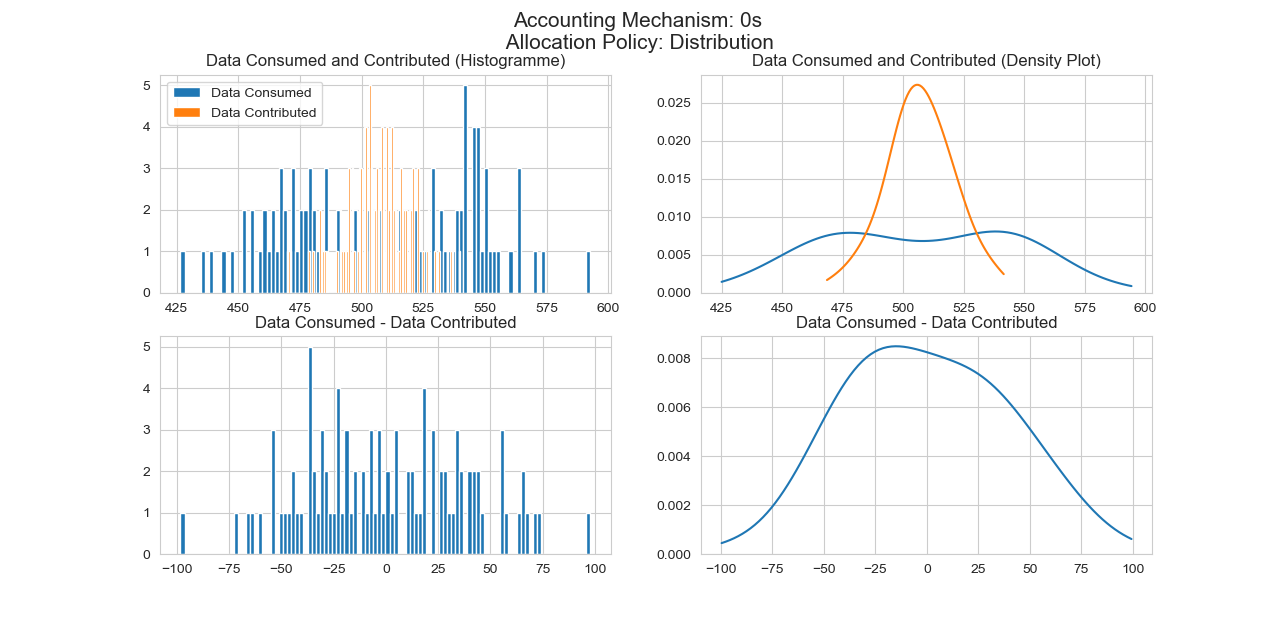
\includegraphics[scale=0.8]{Acc_0s_Dist.png} \\ 
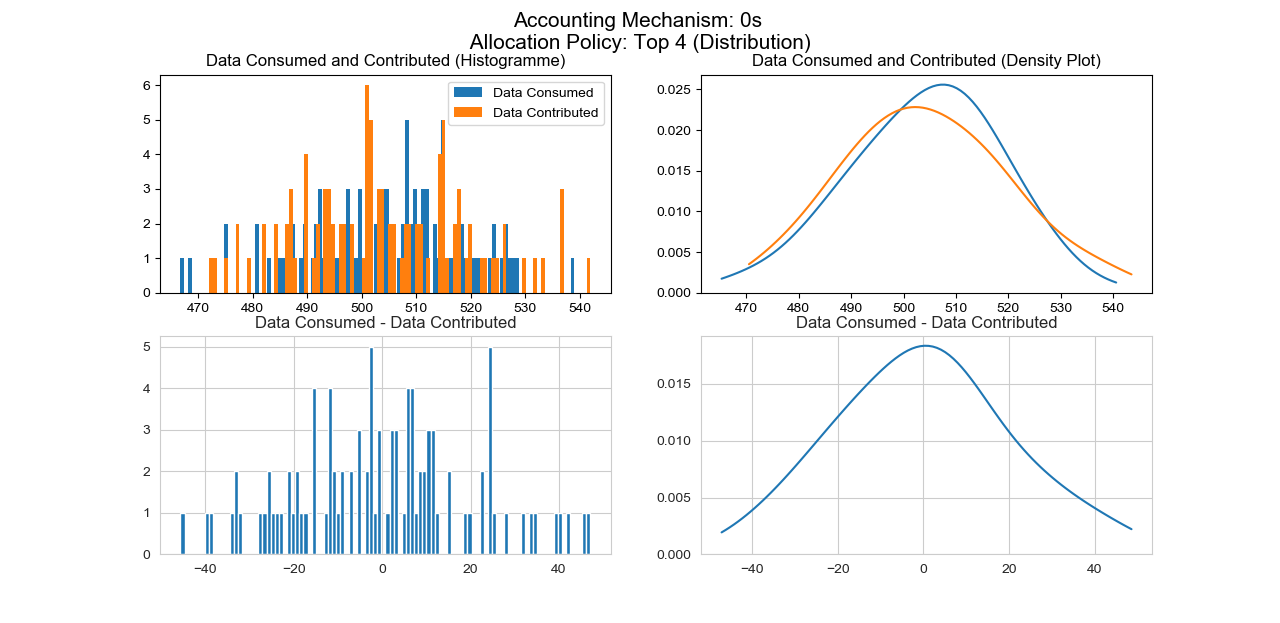
\includegraphics[scale=0.8]{Acc_0s_Top_4_Dist.png} \\
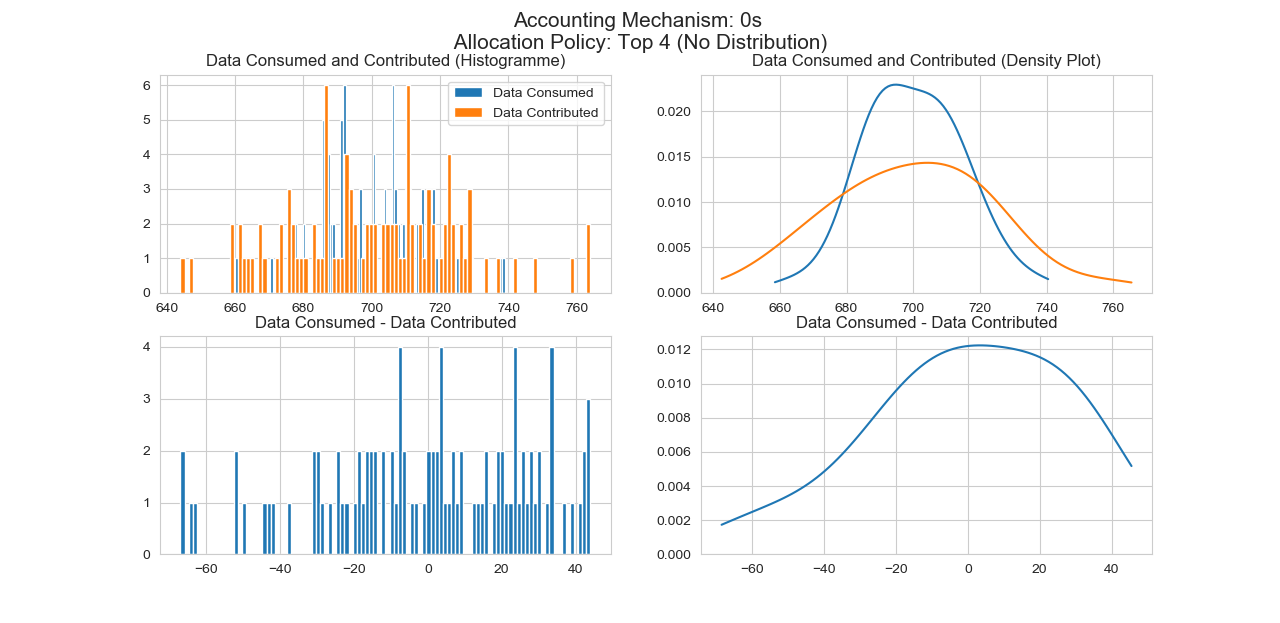
\includegraphics[scale=0.8]{Acc_0s_Top_4_No_Dist.png} \\
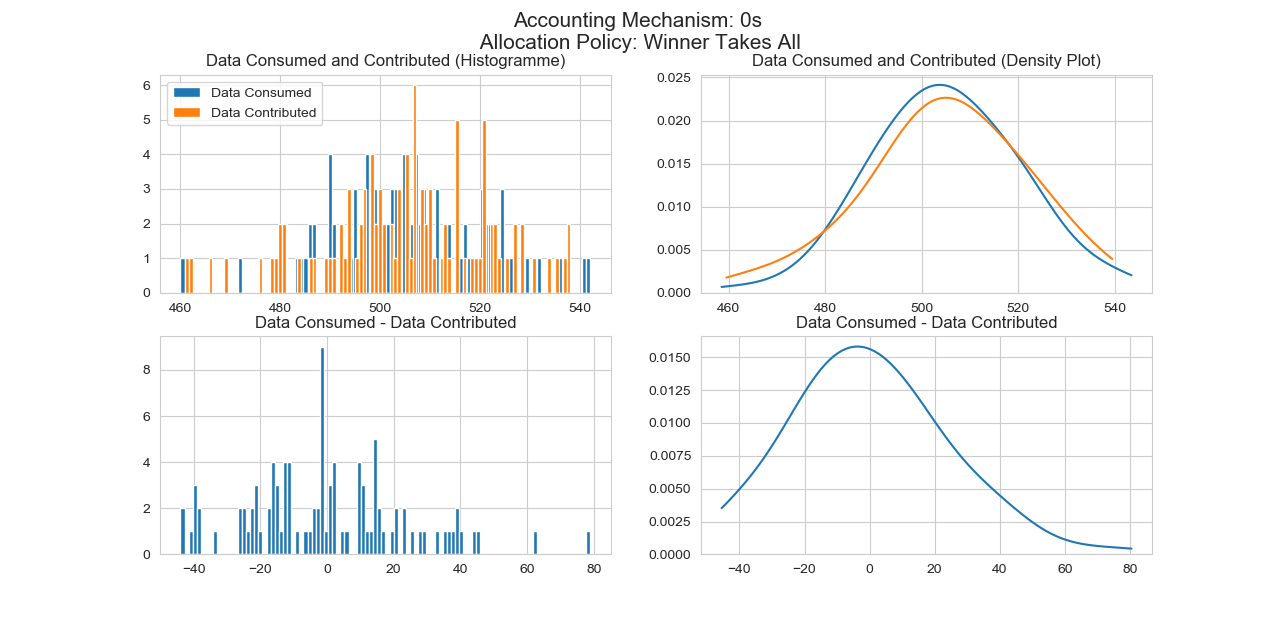
\includegraphics[scale=0.8]{Acc_0s_Winner.png} \\
\end{tabular}
\caption{Simulation values of the Interaction Model given $S^M_i(G_i,j)=0$.}
\label{fig:Acc_0s_Sim_Values}
\end{center}
\end{figure}

\begin{figure}[H]
\begin{center}
\begin{tabular}{c}
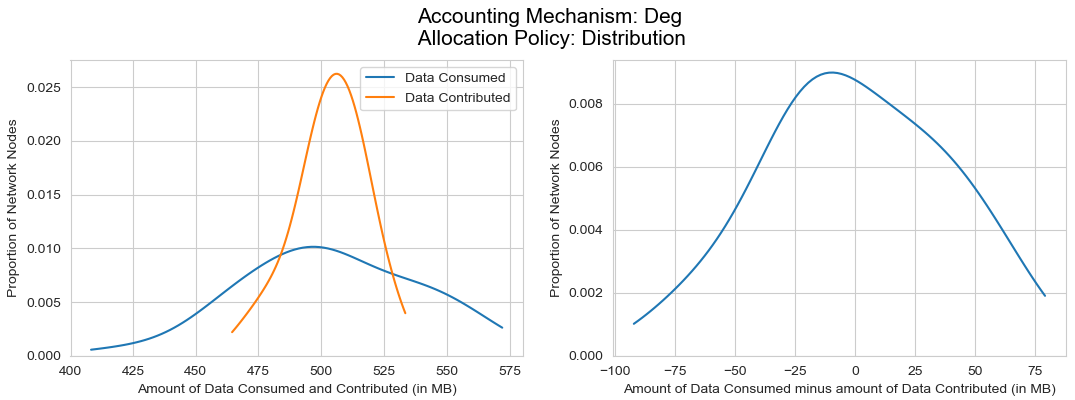
\includegraphics[scale=0.8]{Acc_Deg_Dist.png} \\
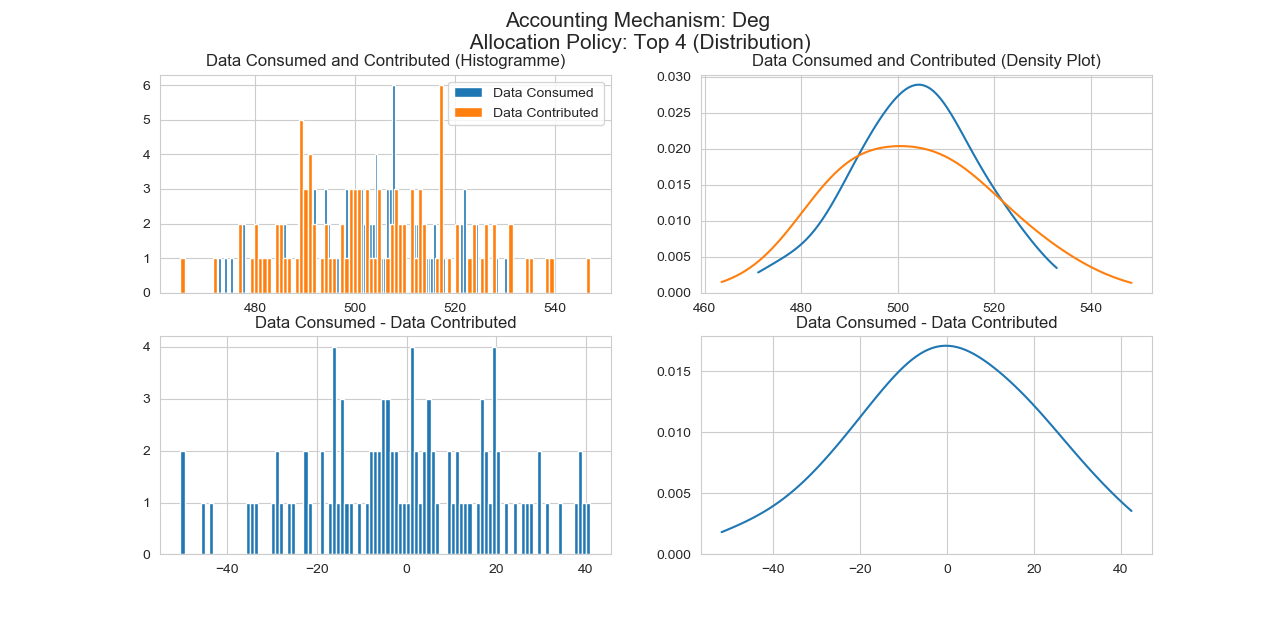
\includegraphics[scale=0.8]{Acc_Deg_Top_4_Dist.png} \\
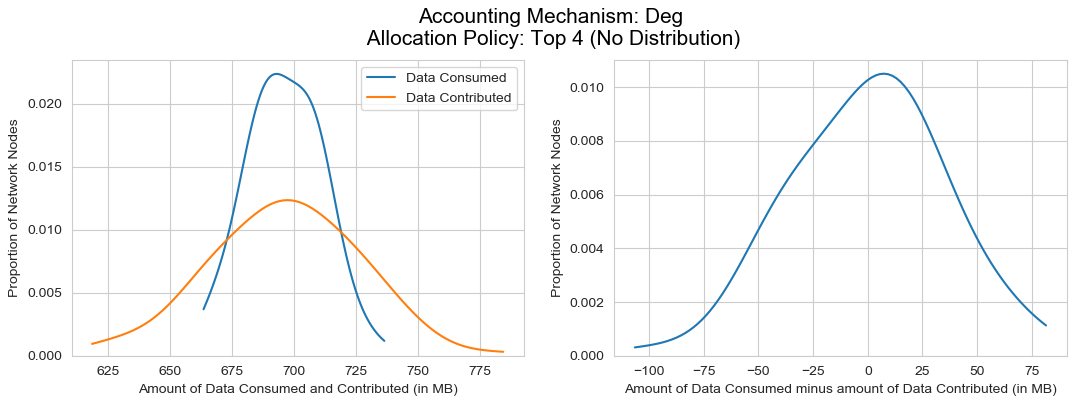
\includegraphics[scale=0.8]{Acc_Deg_Top_4_No_Dist.png} \\
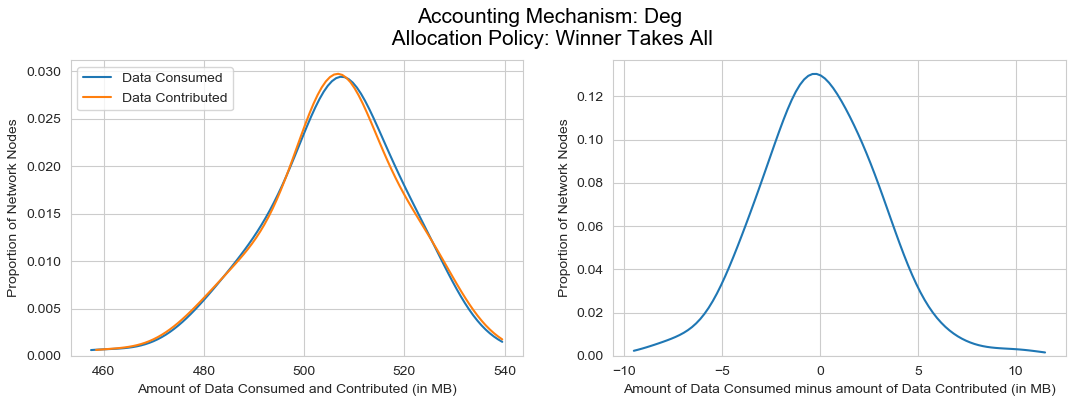
\includegraphics[scale=0.8]{Acc_Deg_Winner.png} \\
\end{tabular}
\caption{Simulation values of the Interaction Model given $S^{Deg}_i(G_i,j)$.}
\label{fig:Acc_Deg_Sim_Values}
\end{center}
\end{figure}

\begin{figure}[H]
\begin{center}
\begin{tabular}{c}
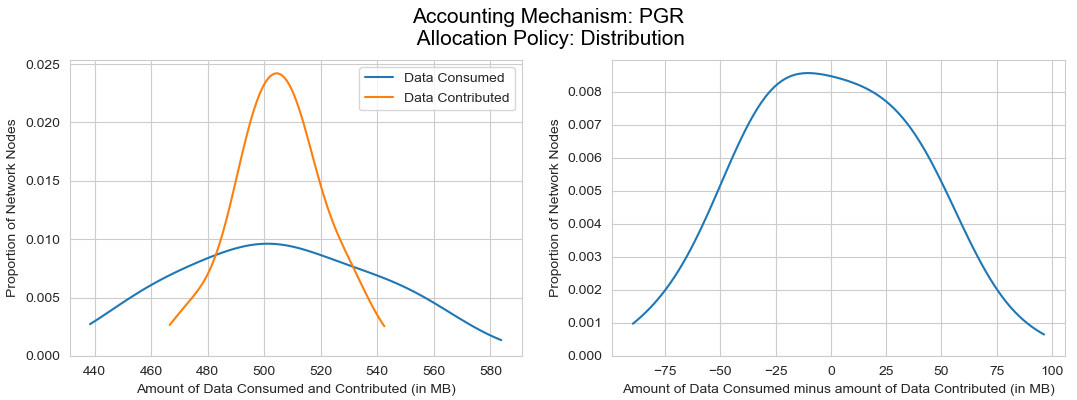
\includegraphics[scale=0.8]{Acc_PGR_Dist.png} \\
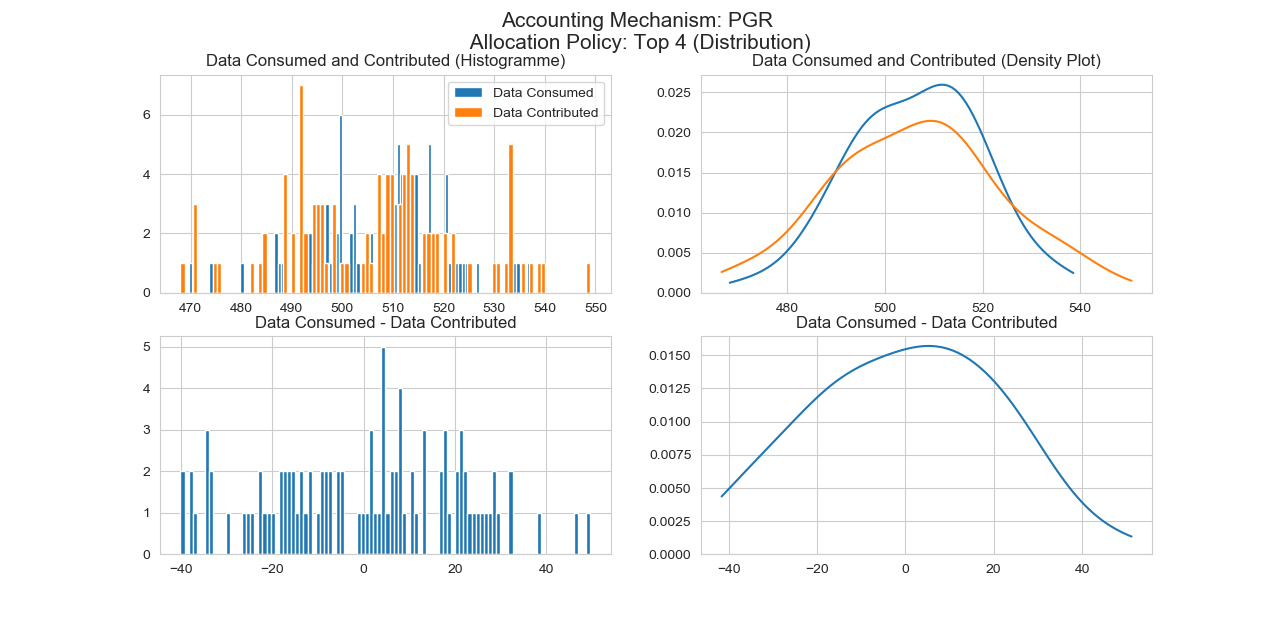
\includegraphics[scale=0.8]{Acc_PGR_Top_4_Dist.png} \\
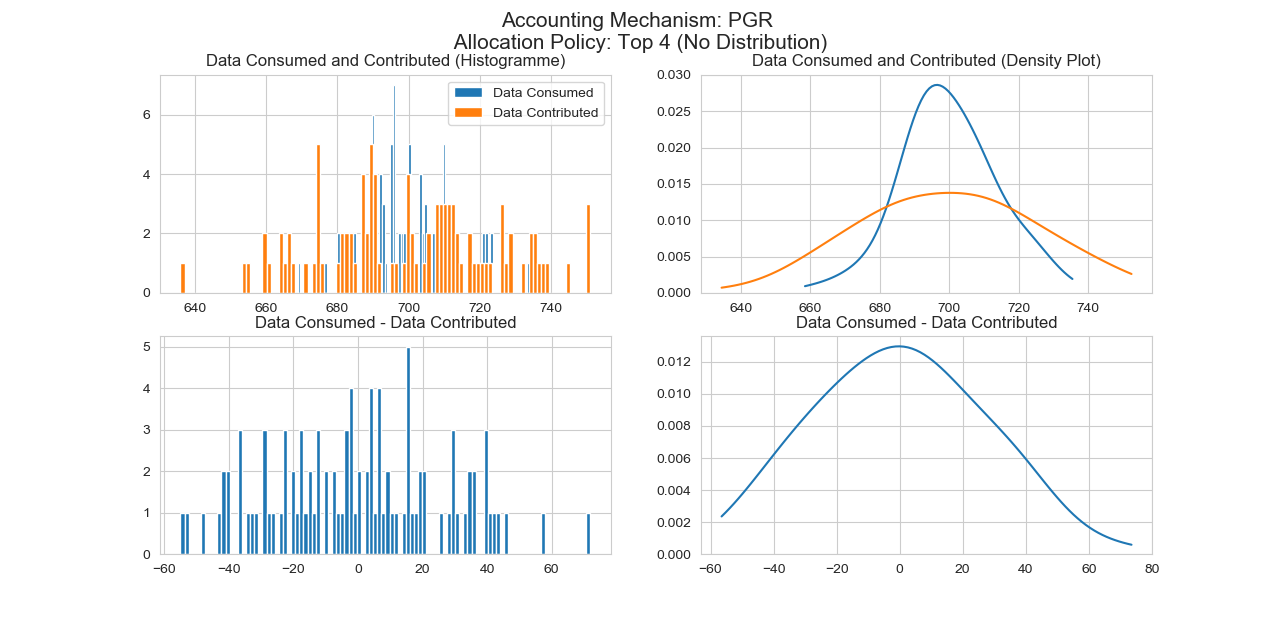
\includegraphics[scale=0.8]{Acc_PGR_Top_4_No_Dist.png} \\
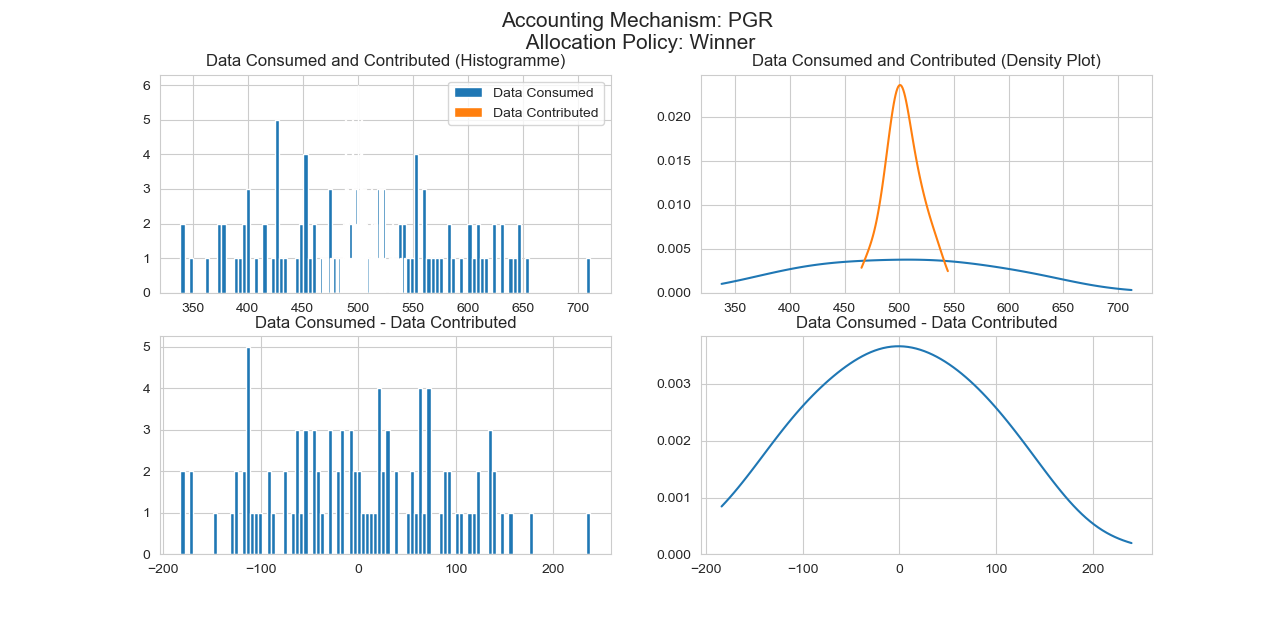
\includegraphics[scale=0.8]{Acc_PGR_Winner.png} \\
\end{tabular}
\caption{Simulation values of the Interaction Model given $S^{PGR}_i(G_i,j)$.}
\label{fig:Acc_PGR_Sim_Values}
\end{center}
\end{figure}


\noindent{}For the simplest accounting mechanism that assigns $0$'s to all nodes in the network, we find that the distribution policy leads to a rather wide-ranging distribution of net contributions made to the network, which implies that the distribution policy is not very effective in preventing or mitigating lazy freeriding. Additionally, we see that the distributions of contributions and consumption are quite different. This means the distribution policy leads to an somewhat inefficient distribution of data in the network and does not reward contributions effectively. The top-4 (distribution) policy does a much better job at preventing lazy freeriding than the distribution policy as we can see from the relatively small variance of the distribution of net consumption in the network. It also leads to a fairer distribution of data. The top-4 (no distribution) policy is even less effective at preventing lazy freeriding and facilitating a fair distribution of data. Lastly, we find that the winner-takes-all policy returns quite nice results for the distribution of net consumption with the exception of two outliers. The distributions of consumption and contribution are also not too different and we conclude that the best allocation policy for the all $0$s accounting mechanism is in fact the winner-takes-all policy. \vspace{1em}\\

\noindent{}For the degree accounting mechanism we find that the distribution policy is very ineffective at punishing freeriders and does not distribute data fairly at all. The top 4 policy without distribution performs equally badly, as can be seen from a rather larger variance in net contributions and unequal distributions of contribution and consumption. The top 4 policy with data distribution is much stronger in both regards with a relatively small variance in the net contributions and similar graphs on the left as well. However, the winner-takes-all policy is by far the best with a extremely small variance in net contributions and almost equal distributions of consumption and contribution. Hence the winner-takes-all policy again is the most effective both in terms of preventing lazy freeriding as well as in facilitating cooperativeness. \vspace{1em}\\

\noindent{}In the case of the personalised PageRank accounting mechanism we find that the distribution policy returns a distribution similar to the distributions we saw for different accounting mechanisms. The fact that the distribution policy always returns very similar distributions of data in the network lies in the fact that every node in the choice set is always served and only the amount the it receives varies depending on its accounting value. The same holds for the top 4 (distribution policy). Although we do observe some differences between its distributions. These may, however be attributed to the randomness of the simulation. As before, the winner-takes-all policy outperforms all other policies, both in preventing freeriding and in rewarding contributions. We note that in terms of rewarding contributions it is outperformed by the top-4 (distribution) policy, albeit by not too much. We conclude this section by noting that the experimental results support our hypothesis and that the winner-takes-all policy is a good choice for the upper interaction model.\vspace{1em}\\

\noindent{}We realise that the set of allocation policies that we investigate is rather limited and that there may be much better allocation policies out there. A possible superior alternative to the winner-takes-all policy could be given by 

\[
A_i(S_i^M(G_i),C_i):=\left\lbrace{} j\in{}C_i\,|\,S^M_i(G_i,j) > 0 \right\rbrace ,
\]

\noindent{}where every node in $A_i(S_i^M(G_i),C_i)$ receives

\[
\tilde{\omega}\cdot\frac{S^M_i(G_i,j)}{\sum\limits_{k\in{}C_i}S^M_i(G_i,k)}.
\]

\noindent{}The reason this allocation policy may be superior to the winner-takes-all policy is that it prevents large-scale sybil attacks, due to the fact that it only serves nodes with accounting values greater than $0$, and therefore sybil nodes will not be served as much. At the same time it does not restrict the distribution to a single node the way the winner-takes-all policy does. For time reasons we did not ffurther investigate this policy. \vspace{1em}\\

\noindent{}Recall that it was the goal of this chapter to define the cost and profit of a sybil attack and so far we have only covered the cost of a sybil attack in definition \ref{def:Sybil Attack Cost}. The reason we took this "detour" to discuss an interaction model and allocation policies is so that we could define the profit of a sybil attack, which we will do now with the upper results on allocation policies in mind.\vspace{1em}\\

 
\begin{definition}[Sybil Attack Profit]\ \\
\label{def:Sybil Attack Profit}
\noindent{}For simplicity of formula we relable $X_{ij}:=S^M_i(G_i,j)$ and define the random vectors $X_i:=(X_{i1},\ldots,X_{in})$ for $i\in{}V$. We define the random variable $Y_{ik}$ as the indicator function which is 1 if $X_{ik}\geq{}X_{ij}$ f.a. $j\in{}C_i$ and $k\in{}C_i$ and zero else. We then define $G'^{(1)}$ as the work graph after the attacker and their sybils have consumed the work they were elligible for after the attack. This continues round for round yielding work graphs $\left(G'^{(n)}\right)_{n\in\mathbb{N}}$. Then we define the expected amount of work node $j$ can consume after sybil attack $\sigma_j^n$ as 

\[
\omega_{+}^{n} = \sum\limits_{n\in\mathbb{N}}\tilde{\omega}\cdot\mathbb{E}\left[\sum\limits_{i\in{}V'\backslash\lbrace{}j,s_{j1},\ldots,s_{j|S|}\rbrace}\sum\limits_{l=1}^{|S|}Y'^{(n)}_{is_{jl}} + Y'^{(n)}_{ij}\right].
\]
\noindent{}At this point, our assumption of an infinite network from \ref{subsec:Interaction Model} comes into play. Without this assumption there would be a possibility that a node $j$ with $S^M_i(G_i,j)=0$ may be served by node $i$ in a particular round, if it is the only node in $i$'s choice set. Therefore, we find that for any node that queries another node with probability $q$ in every round, the upper sum will be infinite. In order to curb this, assumed that while $V_i$ is obviously always finite, there are infinite nodes $u\in{}V$ outside of $i$'s subjective work graph, all with $S^M_i(G_i,u)=0$ that will make queries to other nodes following the same paradigm as above. By this logic the choice set $C_i$ will be of infinite size in every round and the probability of $j$ being served in any given round is arbitrarily small. This results in the sum above being finite for any node in the network that does not "cheat".
\end{definition}

\noindent{}Note that this specification has been completely neglected in the existing literature. In their research Seuken \& Parkes have not specified the values $\omega_{+}^{n}$ and $\omega_{-}^{n}$. However, it is an important one to make, as according to their definition it would always hold $\omega_{+}^n=\infty$. At least for most of the allocation policies discussed in section \ref{chap:Mathematical Framework for Accounting Mechanisms} and therefore any sybil attack would be strongly beneficial with respect to definition \ref{def:Sybil Attack Benefit}. They kept their definition of $\omega_{+}^n$ very vague, referring to it as "the amount of work that agent j or any
of its sybils will be able to consume", but did not specify a time frame \cite{On the Sybil-Proofness of Accounting Mechanisms}. The same applies to $\omega_{-}^n$.\vspace{1em}\\

\noindent{}Otte et al. (2016) solve this problem by assuming an allocation policy called the \textit{strict winner-takes-all policy}, which serves the highest ranking node in the choice set, just like the winner-takes-all policy. However, if all nodes in the choice set have the same accounting values then the strict winner-takes-all policy doesn't serve anyone. We dismiss this allocation policy for the same reasons we disagree with the banning policy in \ref{ex:Banning Policy}, namely that it limits distribution of data in the network.\vspace{1em}\\ 

\noindent{}Now that we have definitions for both the cost and profit of a sybil attack we return to the definition of the benefit of a sybil attack, defined above in definition \ref{def:Sybil Attack Benefit}. Again, we say that a sybil attack is 

\begin{itemize}
\item[] {\bf Strongly Beneficial} if $\omega^n_{+}>0$ and $\omega^n_{-}=0$ or if $\lim\limits_{n\rightarrow\infty}\frac{\omega^n_{+}}{\omega^n_{-}}=\infty$,
\item[] {\bf Weakly Beneficial} if $\omega^n_{+}>0$ and $\omega^n_{-}>0$ and $\exists c>0:\,\,\lim\limits_{n\rightarrow\infty}\frac{\omega^n_{+}}{\omega^n_{-}}\geq{}c$.
\end{itemize}

\noindent{}We inverse these points to introduce sybil resistance.

\begin{definition}[Sybil Resistance]\ \\
\label{def:Sybil Resistance}
\noindent{}Let $j$ be a malicious node perpetrating a sybil attack $\sigma_j^n$ on the work graph $G$, resulting in work graph $G'$. Here $n$ is variable. Now let $\omega_{-}^{n}>0$ denote the cost of the sybil attack $\sigma_j^n$, according to definition \ref{def:Sybil Attack Cost} and let $\omega_{+}^n$ be the sybil attack profit defined in definition \ref{def:Sybil Attack Profit}. Then we call a pair of accounting mechanism and allocation policy $(S^M_i,A_i)$
\begin{itemize}
\item {\bf resistant against strongly beneficial sybil attacks} if 
\[
\forall{}j\in{}V_i\backslash{}\left\lbrace{}i\right\rbrace \forall (\sigma^n_j)_{n\in\mathbb{N}}\,\exists{}c>0:\,\,\lim\limits_{n\rightarrow\infty}\frac{\omega^n_{+}}{\omega^n_{-}}\leq{}c,
\]
\item {\bf resistant against weakly beneficial sybil attacks} if 
\[
\forall{}j\in{}V_i\backslash{}\left\lbrace{}i\right\rbrace \forall (\sigma^n_j)_{n\in\mathbb{N}}:\,\,\lim\limits_{n\in\mathbb{N}}\frac{\omega^n_{+}}{\omega^n_{-}}=0.
\]
\end{itemize}
\end{definition}

\noindent{}Note that sybil-proofness against weakly beneficial attacks is extremely restrictive and very hard to obtain by any form of accounting mechanism, while sybil-proofness against strongly beneficial attacks is easier to achieve and by our standards sufficient for the maintainance of a (mostly) cooperative, functioning network. The reason for this is that while an attacker can launch a sybil attack that returns a multiple of its investment, the idea is that in order for an attacker to leach infinite data, they also have to share infinite data. This means that any form of sybil attack will require some input into the network. No attacker can simply demand all resources in the network, leading to a complete shutdown. Instead, a weakly beneficial sybil attack still stimulates a network enough to maintain its existence. \vspace{1em}\\

\noindent{}Now that we have determined the cost and profit of sybil attacks, we should be able to determine for any pair $(S^M_i,A_i)$ whether it is sybil-resistant or not. However, we remark that due to the probabilistic nature of the the sum in \ref{def:Sybil Attack Profit} it is  impossible to compute for any generic setting making it impossible to determine how effective a sybil attack actually is. We need to renew the upper definitions in a way that makes them more easily computable. \vspace{1em}\\

\noindent{}This brings us to the next section where we reintroduce the profit and cost of sybil attacks in terms of accounting values, instead of work. \vspace{1em}\\


\section{Redefining Cost \& Profit in Terms of Accounting Values}
\label{sec:Cost & Profit in Terms of Accounting Values}
\noindent{}Recall that accounting mechanisms were there to determine the standing of a node in the network and capture how much data an agent is elligible to consume. In a sybil attack it is the goal of the attacker to increase the accounting values of one or more nodes in the sybil region from the perspective of as many honest nodes as possible to be able to consume larger amounts of data from the network. \vspace{1em}\\

\noindent{}In order for us to be able to gauge how profitable an attack is, we introduce another pair of definitions of sybil attack rewards, which we denote $\omega_{+}^{n}$(rep) and $\omega_{-}^{n}$(rep). For uniformity we relabel the former definitions of cost and profit as $\omega_{+}^{n}$(work) and $\omega_{-}^{n}$(work). \vspace{1em}\\ 

\noindent{}In this setting, one might define the reward of an attack $\sigma_j^n$ in terms of accounting mechanisms by the aggregate of accounting values all sybil nodes (including $j$) have collectively obtained through the attack. 

\[
\sum\limits_{i\in{}V'\backslash\left\lbrace{}j,s_{j1}\ldots{}s_{jn}\right\rbrace}\sum\limits_{s\in\left\lbrace{}j,s_{j1}\ldots{}s_{jn}\right\rbrace}S^M_i(G'_i,s).
\]

\noindent{}And we obtain the following definition of sybil attack profit.\vspace{1em}\\

\begin{definition}[Sybil Attack Profit in Terms of Accounting Values]\ \\
\label{def:Sybil Attack Profit (rep)}
\noindent{}Given an objective and a subjective work graph $G:=(V,E,w)$, $G_i:=(V_i,E_i,w_i)$, let $\sigma_j^n$ be a sybil attack of size $n\in\mathbb{N}$ with Sybil region $S=\left\lbrace{}s_{j1},\ldots,s_{jn}\right\rbrace$, whereby $n$ is not fixed. Take $G':=(V',E',w')$ and $G_i':=(V_i',E_i',w_i')$ as defined above. We define $\omega_{+}^{n}$(rep) as the aggregate of accounting values that nodes in the sybil region collectively gain after it has carried out its attack. We obtain

\[
\omega_{+}^{n}({\rm rep}) = \sum\limits_{i\in{}V'\backslash\lbrace{}j,s_1,\ldots,s_n\rbrace}\sum\limits_{s\in\lbrace{}j,s_1,\ldots,s_n\rbrace}S^M_i(G_i',s).
\]
% - \sum\limits_{i\in{}V\backslash\lbrace{}j\rbrace}S^M_j(G_i,C_i)
\end{definition}

\noindent{}We now need to define $\omega^{n}_{-}$(rep). Just as in definition \ref{def:Sybil Attack Profit (rep)} this value needs to be equivalent to the earlier defined $\omega_{-}^{n}$(work), but in terms of accounting values. The reasoning for the definition of $\omega_{-}^{n}$(work) above was that we were trying to capture the amount of work invested into the network by a sybil attacker, i.e. the aggregate of the weights of the attack edges. In terms of accounting values, we can define this concept as the aggregated accounting values a sybil attacker has "earned" through their honest work, invested into the network. \vspace{1em}\\

\begin{definition}[Sybil Attack Cost in Terms of Accounting Values]\ \\
\label{def:Sybil Attack Cost (rep)}
\noindent{}Given an objective and a subjective work graph $G:=(V,E,w)$, $G_i:=(V_i,E_i,w_i)$, let $\sigma_j^n$ be a sybil attack of size $n\in\mathbb{N}$ with Sybil region $S=\left\lbrace{}s_{j1},\ldots,s_{jn}\right\rbrace$, whereby $n$ is not fixed. Take $G':=(V',E',w')$ and $G_i':=(V_i',E_i',w_i')$ as defined above. \vspace{1em}\\

\noindent{}Now we introduce a third graph $G''=(V'',E'',w'')$ where $V''=V$ and $w'':V\times{}V\rightarrow\mathbb{R}$ with $w''(u,v)=w(u,v)$ f.a. $u,v\in{}V\backslash\left\lbrace{}j\right\rbrace$ and $w''(u,j)=\sum\limits_{s\in{}S\cup\left\lbrace{}j\right\rbrace}w'(u,s)$ as well as $w''(j,u)=\sum\limits_{s\in{}S\cup\left\lbrace{}j\right\rbrace}w'(s,j)$. Graphically, this means that we "collapse" all sybil nodes into a single node which we will label $j$ again and all incoming and all outgoing edges from any sybil node into the honest region of the graph, are attached to $j$ in $G''$. \vspace{1em}\\

\begin{figure}[H]
\begin{center}
\includegraphics[scale=0.9]{"Cost Rep(1)".PNG} 
\includegraphics[scale=0.9]{"Cost Rep(2)".PNG} 
\includegraphics[scale=0.9]{"Cost Rep(3)".PNG}
\end{center}
\label{fig:Example of Collapsing a Sybil Region}
\caption{Example of Collapsing a Sybil Region}
\end{figure}

\noindent{}The point is that the aggregate of accounting values that the sybil attacker has gained should be compared to the accounting values that they're actually entitled to based on the actual work performed, i.e. the attack edges. All edges that do not enter or leave the sybil region are therefore disregarded and any increase in reputation that the sybil attackers may gain through the sybil-internal edges is dropped. In formula we then obtain the following value of sybil attack cost \vspace{1em}\\

\[
\omega_{-}^{n}(rep) = \sum_{i\in{}V''\backslash\lbrace{}j\rbrace}S^M_i(G_i'',j).
\]

\end{definition}

\noindent{}We should mention here that we keep the same definitions of sybil attack benefit and sybil resistance as in definitions \ref{def:Sybil Attack Benefit} and \ref{def:Sybil Resistance} in both cases of sybil attack profit and cost. And we call sybil attacks strongly and weakly beneficial in terms of accounting values and in terms of work. \vspace{1em}\\

\chapter{Representativeness of Accounting Mechanisms}
\label{chap:Representativeness of Accounting Mechanisms}



\section{Sybil-proofness of Accounting Mechanisms}
\label{sec:Sybil-proofness of Accounting Mechanisms}



\section{Defining Representativeness}
\label{sec:Defining Representativeness}




\chapter{On the Impossibility of Sybil-Proofness}
\label{chap:On the Impossibility of Sybil-Proofness}



\section{Analysis of Existing Impossibility Results}
\label{Analysis of Existing Impossibility Results}



\section{Improving Existing Impossibility Results}
\label{Improving Existing Impossibility Results}


\subsection{Parallel-Report Responsiveness}
\label{subsec:Parallel-report Responsiveness}


\subsection{Extending the Model to Multiple Hops}
\label{subsec:Extending the Model to Multiple Hops}


\subsection{Serial-Report Responsiveness}
\label{subsec:Serial-Report Responsiveness}







\chapter{Sybil-Proofness of Accounting Mechanisms}
\label{chap:Sybil-Proofness of Accounting Mechanisms}



\section{Characterising Sybil Attacks}
\label{sec:Characterising Sybil Attacks}



\section{Requirements for Sybil-Proofness}
\label{sec:Requirements for Sybil-Proofness}





\chapter{Sybil Resistance Based on Physical Proximity}
\label{chap:Sybil Resistance Based on Physical Proximity}



\section{A Mathematical Framework for Physical Proximity}
\label{sec:A Mathematical Framework for Physical Proximity}



\section{A Two-layered Trust Model}
\label{sec:A Two-layered Trust Model}


\chapter{Conclusion and Discussion}
\label{chap:Conclusion and Discussion}

\noindent{}In this thesis we have examined reputation mechanisms in distributed systems and their resistance to different types of malicious behaviour, whereby we placed the largest emphasis on sybil attacks. We began by introducing a mathematical framework for our research in which we defined fundamental and pertinent concepts such as transaction sequences, work graphs, accounting mechanisms and allocation policies. Thereafter we mathematised different types of malicious behaviour, accounting mechanisms were supposed to prevent, i.e. lazy-freeriding, misreport attacks and sybil attacks. It was our goal to introduce requirements for accounting mechanisms to be resistant to this type of malicious behaviour. \vspace{1em}\\	


\noindent{}We began by investigating \textbf{lazy-freeriding} in chapter \ref{chap:Mathematical Framework for Accounting Mechanisms}. We discovered a combination of requirements that would ensure an accounting mechanism together with an allocation policy could successfully prevent lazy-freeriding. The requirement was called positive-report responsiveness, while the allocation policy had to satisfy the additional constraint of banning any nodes from the choice set with accounting values that exceeded a given lower bound. This resulted in agents, who contributed far fewer resources than they consumed, not being served anymore data by honest agents. Therefore it became impossible for agents to leech excessively.\vspace{1em}\\ 

\noindent{}Next we analysed \textbf{misreports} and the resistance of accounting mechanisms to these types of attacks in the network, whereby we began by critically examining the DropEdge protocol introduced by Seuken \& Parkes \cite{Sybil-proof Accounting Mechanisms with Transitive Trust}. We discovered that this mechanism was only resistant to particular types of misreports which were quite narrowly defined. In response to this discovery we expanded our definition of misreport-proofness and examined the TrustChain data structure in combination with generic gossip protocol. We concluded that TrustChain satisfied a stronger requirement for misreport-proofness for accounting mechanisms, provided that accounting mechanisms satisfied the property of positive-report responsiveness. Given this misreport-proofness we moved on to the most critical issue accounting mechanisms faced, namely sybil attacks. \vspace{1em}\\


\noindent{}The largest emphasis was placed on \textbf{sybil attacks} in this thesis. After having solved the issue of misreports by either the DropEdge mechanism or the TrustChain architecture we moved on to characterising the effects of sybil attacks on P2P networks. We began by defining the cost incurred by the attacker, given by the amount of work that had to be performed for the network and formalised the profit of an attack as well, whereby the profit of a sybil attack was given by the additional amount of work the attacker could consume after the sybil attack had been carried out. The fact that neither profit nor cost of sybil attacks have been rigorously defined up until this point proves itself to be quite problematic and we highlighted the necessity for these definitions. In attempting to determine the profit of such an attack, we realised that we had to determine the expected value of an infinite discrete stochastic process. To solve this problem we postulated an interaction model for nodes in the network. \vspace{1em}\\ 


\subsubsection*{Interaction Model}
\label{subsubsec:Interaction Model}
\noindent{}In order to determine the profit of a sybil attack, we introduced an interaction model by which participants transact with one another and compared the outcome of this interaction model with the real-world {\it Tribler} application. Within the construction of this model we analysed a number of different allocation policies for their resistance to sybil attacks and decided that the winner-takes-all policy was the most suitable in this endeavour. With the now won definiton of sybil attack profit, we realised that computing the value of the expected profit was practically impossible. This prompted us to reformulate the values of cost and profit in terms of the accounting values that sybil attackers were able to obtain. The advantage to this was that the profit in terms of accounting values was, in fact, computable and we were therefore able to gauge the effectiveness of a sybil attack. We did, however incur a problem with this definition. \vspace{1em}\\



\subsubsection*{Representativeness}
\label{subsubsec:Representativeness}
\noindent{}The values of sybil attack cost and profit in terms of accounting values were now much easier to compute. However, they were not actually the relevant metric, but just a proxy for the earlier defined cost and profit of sybil attacks in terms of work. Consequently, we were interested in determining the relationship between the two and came up with two example cases in which the sybil attack benefit converges to infinity in terms of one, but not the other. We learned that the two were not equivalent. This lead to the new definitions of weak and strong {\it representativeness}. After having introduced representativeness, we concluded that any accounting mechanism that is resistant to strongly beneficial sybil attacks in terms of accounting values and is weakly representative, is already resistant to strongly beneficial sybil attacks in terms of work, which was the desired property. \vspace{1em}\\



\subsubsection*{Impossibility Results}
\label{subsubsec:Impossibility Results}
\noindent{}Next, we analysed some existing results in the literature which stated that accounting mechnanisms satisfying independence of disconnected agents, symmetry and single-report responsiveness were \textbf{not} resistant to strongly beneficial sybil attacks in terms of work. We concluded that given our definitions of sybil attack cost and profit this result was incorrect. We corrected the result by adding the requirement of parallel-report responsiveness and added that the consequent sybil susceptibility was in terms of accounting values and not work. If an accounting mechanism satisfied the additional property of strong representativeness then the given sybil susceptibility was also in terms of work. We then extended the model to multiple hops ensuring that the upper assertions were true for arbitrary work graphs. We then introduced another property called serial-report responsiveness and made an analogous assertion. \vspace{1em}\\



\subsubsection*{Sybil-proofing Accounting Mechanisms}
\label{subsubsec:Sybil-proofing Accounting Mechanisms}
\noindent{}Using the impossibility results we arrived at in chapter \ref{chap:On the Impossibility of Sybil-Proofness}, we realised we could characterise passive sybil attacks as parallel and serial attacks and a combination of the two, which we called pyramid attacks. We inverted the concepts of parallel- and serial-report responsiveness to obtain resistance against these types of attacks. Thereafter we introduced the very important definition of multiple-path response bound from which we concluded that the profit in terms of accounting values of any sybil attack could be bounded by the profit of some pyramid attack, multiplied by a constant. This lead to the final result that any accounting mechanism satisfying the upper properties was resistant against strongly beneficial sybil attacks in terms of accounting values, which in combination with weak representativeness implied resistance to strongly beneficial sybil attacks in terms of work.\vspace{1em}\\ 

\noindent{}Given these results we believe that we have adequately answered the research question from chapter \ref{chap:Introduction} \vspace{1em}\\

\begin{center}
{\it What requirements does an accounting mechanism need to satisfy in order to effectively incentivise cooperation and prevent lazy freeriding, while being resistant to misreport attacks and mitigating the effects of sybil attacks?} \vspace{1em}\\
\end{center}

\section{Future Work}
\label{sec:Future Work}
\noindent{}In this thesis we covered a wide array of problems in the context of cooperation in P2P file sharing networks. We are particularly pleased with some of our results on the theoretical properties accounting mechanisms and allocation policies must satisfy in order to achieve sybil-proofness. Given the time constraints of a master thesis project, some of our research was cut short a bit. In this section we would like to elaborate a little bit on possible future work that could be conducted in researching the problems this thesis covered. \vspace{1em}\\

\subsubsection*{Allocation Policies}
\label{subsubsec:Allocation Policies}
\noindent{}The research on allocation policies we conducted within defining the sybil attack profit in terms of work, has been rather slim and  did not reach a final strong conclusion. We determined that out of the allocation policies introduced in chapter \ref{chap:Mathematical Framework for Accounting Mechanisms} the winner-takes all was the most sybil resistant and lead to the fairest distribution of data in the network as was seen in the experiments conducted in \ref{subsec:Experimental Evaluation}. In future work, one may want to formalise a more generic set of sensible allocation policies and determine the optimal policy out of this set. One may determine a set of allocation policies given by convex combinations of the top $n$ policies, i.e. combinations of distribution and top $n$ policies where the highest ranking $n$ nodes will be served each with an amount of work corresponding to their standing in the choice set. If combined with some banning element, whereby only nodes with accounting values greater than a given upper bound are served, such allocation policies may succeed in preventing both lazy freeriding and sybil attacks. Research on allocation policies to our knowledge has been rather scarce and may be a topic of research that hides promising results.\vspace{1em}\\

\subsubsection*{Resistance Against Weakly Beneficial Sybil Attacks}
\label{subsubsec:Resistance Against Weakly Beneficial Sybil Attacks}
\noindent{}The research conducted for this thesis was all done with P2P file sharing networks in mind, more precisely the {\it Tribler} application. In this setting weakly beneficial sybil attacks are not by any stretch of the imagination disastrous for the network. The reason for this is that in filesharing networks a weakly beneficial sybil attack in terms of work requires the attacker to invest infinite resources in order obtain infinite resources. This renders weakly beneficial sybil attacks comparatively harmless. No single malicious agent can simply demand all, or even a significant proportion of the resources in the network. However, other types of P2P networks such as social networks may not have such resistant properties. If one thinks of a sybil attacker on Facebook that aims to spread fake news by tricking the network into considering their content more relevant for people's feeds than it actually is. In such a case, a weakly beneficial sybil attack may have disastrous consequences. For future work it may be very nice to obtain some stricter finite upper bounds on the benefits of sybil attacks. For this, one could start of by tightening the definitions of parallel- and serial-report convergence to obtain a limit $\leq{}c$ for some $c>0$. \vspace{1em}\\

\subsubsection*{Expanding on Representativeness of Accounting Mechanisms}
\label{subsubsec:Expanding on Representativeness of Accounting Mechanisms}
\noindent{}In chapter \ref{chap:Representativeness of Accounting Mechanisms} we introduced the concept of representativeness of accounting mechanisms. The idea was that accounting values were simply a representation of the reputation of nodes in the network and therefore a proxy for the amount of work these nodes were entitled to. We incurred the problem of sybil attacks which were strongly beneficial in terms of accounting values but not in terms of work, and vice versa, prompting us to make the restriction for accounting mechanisms to have to satisfy at least weak representativeness in order to be sensible. In remark \ref{rem:Representativeness Function} to further elaborate on what requirements accounting mechanisms must satisfy in order to be weakly and strongly representative we explained the concept of a representativeness function, but did not delve further into this issue. It is, however a crucial point in the resistance to sybil attacks. In future work one may want to further identify properties representative accounting mechanisms satisfy and make consequent additional restrictions to be able to better identify sensible accounting mechanisms.\vspace{1em}\\ 

\section{Further Discussion and Ethical Ramifications}
\label{sec:Further Discussion and Ethical Ramifications}
\noindent{}The research question of this thesis has far-reaching implications and may find application in many types of networks other than just P2P filesharing networks. Digital currencies may be one of these, where the accounting values would not necessarily reflect an agent's trustworthiness, but instead the balance of their account, i.e. the amount of digital money they own. Another preeminent setting for accounting mechanisms to find application in, are online social networks. Networks such as Facebook and Twitter struggle to clamp down on the spreading of hateful speech and fake news. Malicious agents may decide to create many fake accounts which all "follow" or "like" one another in order to boost the probability of their content being seen by many people. The algorithms of these companies that decide whose content is recommended and shown on other honest agents' feeds so far have been very susceptible to these types of attacks. Online social networks try to shut down attacks like this with the help of machine learning algorithms that are trained to detect fake accounts. However, oftentimes mistakes are made and anyone who has used these services has witnessed this first hand. Companies running these services may want to consider broadening their set of tools with which they tackle these attacks by sybil-proof accounting mechanisms that represent the trustworthiness of agents in the network. \vspace{1em}\\

\noindent{}One more application that has occured to us throughout the process of this research have been real-life social scoring systems. Countries like China have introduced social credit systems with which they aim to rate their citizens trustworthiness. Bad behaviour of citizens will lead to lower scores while good behaviour will increase respective scores \cite{Big Data Meets Big Brother as China Moves to Rate its Citizens}. These scores are then used by the government to allow their citizens different levels of liberty, whereby lower ranking citizens are restricted in their freedom. From a western libertarian perspective this extent of government surveillance seems obviously unethical (of course this is debatable). We are aware of the fact that our research in the direction of social reputation scores may assist oppresive regimes in constructing social accounting mechanisms to enhance their control over peoples' lives. Of course, we realise that our research is only very peripherally related, nevertheless we feel that this must be pointed out and further research in this direction should be conducted with some level of caution and awareness of its ethical consequences.\vspace{1em}\\

\begin{comment}
\begin{itemize}
\item Future Research: Different Allocation Policies: Our research on allocation policies has been mostly inconclusive, figure out which allocation policy is most sybil resistant; We only covered \textbf{strongly} beneficial sybil attacks because of the P2P filesharing system in mind; In other types of networks this may not be sufficient at all, think about introducing an upper bound for sybil attack profit under certain conditions; Maybe mention that pur definitions of sybil attack cost and profit are based on our personal intuition, i.e. they just kinda make sense to us ... lol. Say that under other definitions of these, the whole thing may look very different.

\item Applications: P2P filesharing, obviously; Other types of P2P networks such as currency systems maybe; Social networks (big problems there with fake news propagation and fake account stuff); Social scoring systems ... tongue-in-cheek (this does make us think)

\item Ethical Ramifications of our research; An important thing here is that it could be theoreticall used for social accounting, malicous governments may use these things to track and alayse people. This is fucked up!
\end{itemize}
\end{comment}

%% Use letters for the chapter numbers of the appendices.
\appendix

\chapter{Appendix}
\label{chap:Appendix}

\section{Reputation Dynamics in Indirect Reciprocity}
\label{sec:Reputation Dynamics in Indirect Reciprocity}

\subsection{Axioms defining Reputation Mechanism}
\label{subsec:Axioms defining Reputation Mechanism}
In order for us to determine what properties a reputation mechanism needs to satisfy we looked into evolutionary biology. In \cite{How Should we Define Goodness} the concept of a binary honour score coupled with a set of behavioural strategies is introduced. An honour score is based not on a node's entire transaction history, but on its most recent transaction. The set of honour scores is given by $\{0,1\}$ and the set of strategies by $\{C,D\}$ , whereby $C$ stands for cooperate and $D$ for defect. It has been shown that conditional and unconditional altruism leads to cooperation among a population. Every node has a reputation value of either 0 or 1 and every node has a behavioral strategy, given by 
\[
p:\{0,1\}^2\rightarrow{}\{C,D\}.
\]
$p$ determines whether a node with a given reputation value will cooperate with a node of another reputation value. For instance $p(0,1)=C$ means that a node with reputation value 0 will cooperate with a node of reputation value 1. A reputation dynamic is a function that assigns a node that has made a decision whether to cooperate or defect with another node a new reputation value, i.e.
\[
d:\{0,1\}^2\times{}\{C,D\}\rightarrow{}\{0,1\}.
\]
In this case for instance $d(0,1,C)=1$ implies that if a node of reputation 0 cooperates with a node of reputation 1 then it will be assigned reputation 1. \vspace{1em}\\
This yields $2^8$ possible reputation dynamics and $2^4$ behavioural strategies. Note that a reputation dynamic is fixed and population dependent whereas a behavioural strategy is personal and node-specific. \vspace{1em}\\

\noindent{}Ohtsuki et al. identify a number of beahvioural strategies and reputation dynamics of particular importance \cite{How Should we Define Goodness}.

{\centering
\begin{figure}[H]
\begin{center}
\includegraphics[scale=0.6]{"Behavioural Strategies".png}
\end{center}
\label{fig:BehvaiouralStrategies}
\caption{Behavioural Strategies (taken from \cite{The leading eight: Social norms that can maintain cooperation by indirect reciprocity}).}
\end{figure}
}

{\centering
\begin{figure}[H]
\includegraphics[scale=0.6]{"Reputation Dynamics".png}
\label{fig:ReputationDynamics}
\caption{Reputation Dynamics (taken from\cite{The leading eight: Social norms that can maintain cooperation by indirect reciprocity}).}
\end{figure}
}

\subsection{Requirements for Reputation Mechanisms}
\label{subsec:Requirements for Reputation Mechanisms}

\noindent{}A combination of reputation dynamic and behavioural strategy $(p,d)$ is called evolutionary-stable strategy (ESS) if $p$ is evolutionarily stable among all 16 possbile behavioural strategies given the reputation dynamic $d$. This means that given the reputation dynamic $d$ the behavioural strategy $p$ receives on average the highest payoff among all other 15 behavioural strategies, given that the population is dominated by agents with the same behavioural strategy, i.e. more than $50\%$ of the network exhbibit the same strategy. As a corollary statement this implies that the benefit of increasing one's reputation must exceed the cost of the work performed for this increase in reputation. An ESS is a refined form of a Nash equilibrium.\vspace{1em}\\

\noindent{}We assume that participating in a P2P-filesharing network constitutes a multi-player game-theoretical game, given by $\mathcal{G}_n=(S,d,E)$ where $n$ is the number of participants, $S=\left\lbrace{}p_i:\{0,1\}^2\rightarrow{}\{C,D\}|1\leq{}i\leq{}n\right\rbrace$ is the set of behavioural strategies of all agents in the network. $E(p,S)$ is then the expected payoff or profit of an agent with behavioral strategy $p$ in the network $\mathcal{G}_n$. Note that this payoff function is a stochastic expected value and not deterministic, because it depends on who the agent interacts with. This expected payoff is given by $\mathbb{E}[b(p_X(r(X),r(i))]-\mathbb{E}[c(p_i(r(i),r(X))]$, whereby $X$ is a random variable choosing players in the network with a predetermined probability distribution $f_X$, $b$ and $c$ correspond to the benefit and the cost of a possible cooperation and/or defection. \vspace{1em}\\

\begin{definition}[ESS Strategy]
The expected payoff of a player with strategy $p$ in a network where $l$ of the $n-1$ remaining nodes play with the strategy $p$ and $n-1-l$ of the players play with strategy $q$, can be written $E(p,p^l,q^{n-1-l})$. A strategy $p$ is said to be evolutionarily stable with respect to another strategy $q$ if there exists a $j\in\left\lbrace{}1,\ldots,n-1\right\rbrace$ such that
\begin{align}
&\forall{}i\leq{}j:\,\,E(p,p^{n-1-i},q^i)\geq{}E(q,p^{n-1-i},q^i)\\
&\forall{}i>j:\,\,E(p,p^{n-i-1},q^i) > E(q,p^{n-i-1},q^i).
\end{align}
A strategy $p$ is then called evolutionarily stable if it is evolutionarily stable with respect to all strategies $q\neq{}p$. \vspace{1em}\\
\end{definition}
\noindent{}Note that we also allow for mixed strategies as well, whereby an agent may choose to play with strategy $p$, $x\%$ of the time and strategy $q$, $1-x\%$ of the time. This can be extended to countably finite convex combinations of pure strategies, as defined in \cite{Game Theory}. However, so far we have only worked with finite strategy spaces, which leads to finite convex combinations. \vspace{1em}\\

\noindent{} Note that the payoff function above is stochastic. This is because opponents / interaction partners are chosen at random and therefore the strategy of the opponent is not deterministic. Note that in our evaluation we assume a uniform distribution for partner choice. \vspace{1em}\\

\noindent{}The concept of evolutionarily stable strategies originated in evolutionary biology. Intuitively it means that a population of players with a particular strategy $p$, if invaded by a minority of players with a new/different strategy $q$ (genetic mutants), is resistant to the propagation of this strategy as a superior one (spread of genetic mutation). Applied to the context of P2P file-sharing, this means that no subset of cheaters can overrule the network, making it unusable for honest/cooperative players, through a dishonest strategy.\vspace{1em}\\  

\noindent{} Ohtsuki et al. (2004) introduce a direct and an indirect observation model. In our case, because of TrustChain we can assume a direct observation model \cite{How Should we Define Goodness}. 


{\centering
\begin{figure}[H]
\begin{center}
\includegraphics[scale=0.6]{"ESS Pairs".png}
\label{fig:ESS Pairs}
\caption{ESS Pairs (taken from \cite{The leading eight: Social norms that can maintain cooperation by indirect reciprocity})}
\end{center}
\end{figure}
}


\subsection{Leading 8}
\label{subsec:Leading 8}
Ohtsuki (2004) identify a set of ESS strategies, which they refer to as the {\it leading eight}, which have a relative payoff of over $94\%$. These are ESS pairs regardless of the cots-to-benefit ratio of transactions, so long as $b>c$. This is not the case for any other pair $(d,p).$ They are also ESS, independently of error rates. The leading 8 are characterised by the following properties, which they all satisfy.
\begin{figure}[H]
\begin{center}
\begin{tabular}{|c|c|c|c|c|c|}
\hline & & & & \\[-0.7ex] $d_{*1C}$: & $d_{*1D}$: & $d_{10D}$: & $d_{11D}$: & $d_{01D}$: \\[1.5ex] \hline & & & & \\[-0.7ex]
$=1$ & $=0$ & $=1$ & $=0$ & $=0$ \\[1ex]\hline
\end{tabular}
\label{fig:Leading 8 strategies}
\caption{Leading 8 strategies (taken from \cite{The leading eight: Social norms that can maintain cooperation by indirect reciprocity}).}
\end{center}
\end{figure}


\noindent{}During our research visit to Sokendai Graduate School of Advanced Studies it was our goal to discuss these leading 8 with the authors of \cite{The leading eight: Social norms that can maintain cooperation by indirect reciprocity} and determine how we could apply these  concepts to our research of facilitating cooperation in P2P filesharing networks. The idea was to determine the crucial properties of the leading 8 and determine a reputation mechanisms in P2P filesharing networks that would satisfy these in the hopes that it would facilitate cooperation in that setting as well, i.e. prevent lazy freeriding. The problem we stumbled upon was that the reputation dynamics defined above were all binary, however we wanted our accounting mechanisms to be continuous, such that we could set up a ranking of nodes in the network, for agent to decide whom to contribute to. All attempts to make the upper reputation dynamics continuous without losing the cooperation-facilitating properties were in vein and we decided to pursue research in a different direction. Another problem we incurred was the fact that the reputation dynamics given above were all global. By this we mean that agents held a reputation value that all other agents in the network agreed upon. However, our accounting mechanisms were designed to be personalised, i.e. every agent assigns other agents in the network respective trust scores. It even occurred to us that for global reputation values in a networks it was impossible to achieve any kind of sybil-proofness. We could not reconcile these issues with our topic of research. \vspace{1em}\\





\section{Sybil Resistance Based on Physical Proximity}
\label{sec:Sybil Resistance Based on Physical Proximity}
\noindent{}Recall that while incentivising cooperation through an accounting mechanism was our primary focus, we had to prevent agents from gaming the accounting mechanism through sybil attacks as introduced in chapter \ref{chap:Mathematical Framework for Accounting Mechanisms}. We wanted to be able to determine whether a group of nodes is, in fact, controlled by one and the same entity. It's extremely difficult to do this, only by looking at the subjective work graph of a participant. After considering a number of different attributes of nodes in the network that may be helpful in determining whether a set of nodes belong to the same agent in the network, we concluded that one such attribute may be their geographic location. We can determine whether a set of nodes is controlled by the same entity by determining and cross-referencing their respective IP adresses, or location in the Internet layer. In order to keep it as generic as possible, we introduced the notion of a {\it similarity vector} as a vector of attributes of a set of nodes that may hint at their likelihood of being controlled by the same entity. These could include values such as IP-address, Ping times from different established nodes as well as properties such as traceroutes, etc.  \vspace{1em}\\

\begin{definition}[Similarity Vector]\ \\
Given the set of agents in the network $V$ and an agent $i\in{}V$, we call $p_i$ a similarity vector if it has a set of properties such that if another set of sybil identities created by $i$, $S_i=\left\lbrace{}s_{i1},\ldots,s_{in}\right\rbrace$ all satisfy $\|p_{s_{ij}}-p_i\|<\varepsilon$ f.a. $j\in\left\lbrace{}1,\ldots,n\right\rbrace$ for a given, fixed $\varepsilon > 0$. The exact properties of such a similarity vector will be discussed later. % $p_i:{\left\lbrace 0,1\right\rbrace}^{128}\times{}PK$
\end{definition}

\begin{definition}[Proximity Graph]\ \\
Given a set of vertices $V$ and a set of corresponding similarity vectors $\left\lbrace{}p_i\,|\,i\in{}V\right\rbrace$ we derive what we call a proximity graph $G_{Pr}:=(V,E)$, which is an undirected, unweighted graph, whereby for $i,j\in{}V$ we set $(i,j)\in{}E\Leftrightarrow\|p_i-p_j\|<\varepsilon$. Note that the proximity graph being undirected implies $(i,j)\in{}E\Leftrightarrow(j,i)\in{}E$.
\end{definition}

\noindent{}Nodes need to be able to cross-reference the similarity vectors (IP-adresses, etc.) of a group of nodes they find suspicious and subsequently group together nodes that are likely to be controlled by a single identity. Analogously to the aforementioned work and trust graphs, agents do not have full knowledge on the entire proxmity graph either. Instead, nodes have a subjective proximity graph, based on agents sharing/reporting their own respective similarity vectors to one another. Agents construct a subjective proximity graph based on the information that is available to them. \vspace{1em}\\

\begin{definition}[Agent Information]\ \\
Every node 'knows' about a subset of all similarity vectors in the network, i.e. agent $i$ has a set $S_i:=\left\lbrace{}p^{(i)}_j\,|\,j\in{}V^{(i)}\right\rbrace$ with $V^{(i)}\subset{}V$.
\end{definition}
\noindent{}From this subjective agent information every node constructs its own subjective proximity graph.
\begin{definition}[Subjective Proximity Graph]
Given a proximity graph $G_{Pr}=(V,E)$ with similarity vectors $\left\lbrace{}p_j\,|\,j\in{}V\right\rbrace$ an agent $i$ with agent information $S_i$ has the subjective proximity graph $G_{Pr}^{(i)}=(V^{(i)},E^{(i)})$ with $V^{(i)}\subset{}V$ and $E^{(i)}:=\left\lbrace{}(i,j)\,|\,\|p^{(i)}_j-p_i\|<\varepsilon\right\rbrace$.
\end{definition}


\noindent{}Note that the individual input values of this similarity vector may vary and can be determined based on what is deemed important information. In the case of the Tribler networks one should definitely include IP address, i.e. location in the network graph, as well as ping times from different nodes. One may even want to include some established nodes that are considered trustworthy who will ping new agents and report respective ping times to all other nodes. The point is that every component of the similarity vector will have some notion of a norm on it, i.e. one can measure distance in terms of ping times or in terms of hops in the traceroute tree. This norm will be applied to the similarity vectors to determine the neighbourhoods of nodes in the proximity graph. \vspace{1em}\\ 

\noindent{}Now knowing that we have two respective graphs that we can work with, we introduce a two-layered trust model.\vspace{1em}\\

\subsection{A Two-Layered Trust Model}
\label{subsec:A Two-Layered Trust Model}
Our model so far has consisted of an agent $i$'s subjective work graph $G_i$, a choice set $C_i$, an accounting mechanism $S^M(G_i,C_i)$ and an allocation policy $A_i(S^M(G_i,C_i))$. From this information, we derived a node or a set of nodes for $i$ to contribute to. 

\begin{figure}[H]
\begin{center}
\includegraphics[scale=0.9]{"One-layer trust model".png}
\caption{One-Layer Trust Model}
\label{fig:One-Layer Trust Model}
\end{center}
\end{figure}

\noindent{}Now, we have a two-layered trust model, in which we are given a work graph and, using our notion of a similarity vector, we determine a proximity graph. Using this proximity graph we derive a newly formed subjective work graph. Then, using our existing accounting mechanisms and allocation policies, we determine a set of nodes to contribute to, analogously to our previous one-layer-model. \vspace{1em}\\

\begin{figure}[H]
\includegraphics[scale=0.7]{"Two-layer trust model".png}
\caption{Two-Layer Trust Model}
\label{fig:Two-Layer Trust Model}
\end{figure}
\noindent{}The idea is that using our proximity graph, we derive our subjective work graph, by collapsing all nodes in the subjective work graph that are connected in the proximity graph. \vspace{1em}\\

\begin{definition}[Collapsing nodes in the work graph]
Given a subjective work graph of agent $i$, $G_i=(V_i,E_i,w_i)$ and a subjective proximity graph of $i$, $G^{(i)}_{Pr}=(V^{(i)}, E^{(i)})$, with $V_i=V^{(i)}$, $i$ derives a new subjective work graph from $G^{(i)}_{Pr}$, by collapsing all nodes in $G_i$ that are connected in $G^{(i)}_{Pr}$. This means we obtain a new graph $G'_i:=(V'_i, E'_i, w'_i)$ with $|V'_i|\leq{}|V_i|$ such that
\[
\forall{}i\in{}V^{(i)},\,\neg\exists{}j\in{}V^{(i)},(i,j)\in{}E^{(i)}\,:\,i\in{}V'_i\,\,\&\,\,(i,j)\in{}E'_i\,\,\&\,\,w'_i(i,j)=w_i(i,j) .
\]

\[
\forall{}i\in{}V^{(i)},\,\exists{}j\in{}V^{(i)},(i,j)\in{}E^{(i)}\,:\,\forall{}j\in{}N_{pr}(i)\cup{}\lbrace{}i\rbrace,\,j\not\in{}V'_i,\forall{}j,k\in{}N_{pr}(i), (j,k)\in{}E_i\,:\,(j,k)\not\in{}E'_i,\,\tilde{i}\in{}V'_i.
\]
This means that, any node in the subjective work graph, which does not have any neighbours in the proximity graph is adopted into the new subjective work graph, while any nodes that are connected in the proximitiy graph, are assigned a "proxy" node $\tilde{i}$ in the new work graph, and all edges connecting nodes in a neighbourhood of the subjective work graph are dropped. The outgoing and incoming edges of the neighbourhood of $i$ are now attached to $\tilde{i}$ in the new subjective work graph. \vspace{1em}\\
\end{definition}

\noindent{}Now we have obtained a new subjective work graph in which all sybil nodes (with a given probability) have been collapsed into a single node. Given this new subjective work graph, agents can run the same accounting mechanisms as before and determine agents' respective accounting values and then determine who to contribute to. If any node that has been removed or collapsed in the subjective work graph now queries an honest node for data, it will not be served and agents that attempt to boos their accounting values through sybil attacks will not be able to increase these values significantly, provided the similarity vectors and the norms have been rigorously defined.\vspace{1em}\\

\noindent{}If the similarity vector only consists of IP-addresses we aim to find a mechanism with which nodes can prove to have different IP-addresses from other nodes without revealing their identities. For this we work with the concept of a hash function from the space of possible IP-addresses to the space of public keys.

\begin{definition}[Hash Function]\ \\
Let $PK:=\left\lbrace \right\rbrace$ be the set of public keys in the P2P network {\it tribler} and let ${\left\lbrace{}0,1\right\rbrace}^{128}$ be the set of IPv6 addresses, comprising 128-bit values. We define the hash function $H:PK\rightarrow{\left\lbrace{}0,1\right\rbrace}^{128}$ as a one-way encryption function satisfying the following 3 conditions:
\begin{itemize}
\item Preimage Resistance: Given a value $y$ in the codomain of $H$, it should be computationally infeasible to determine a value $x\in{}PK$ such that $H(x)=y$. More precisely, in our case it should take $\mathcal{O}(2^{128})$ time to determine the preimage of $y$.
\item Second Preimage Resistance: Given a value $x$ in the domain it should be equally difficult to determine another $x'$ satisfying $H(x)=H(x')$.
\item Collision Resistance: Given our hash function it should be computationally infeasible to determine two values $x$ and $x'$ such that $H(x)=H(x')$. To find such a collision an expected $\sqrt{2^{64}}$ tries are needed. This is due to the birthday paradox, which is introduced by \cite{Cryptography made simple}. 
\end{itemize}
\end{definition}

\begin{definition}[Neighbourhood of a node]\ \\
\noindent{}A node $i$ that bootstraps in the network then computes the hash of its IP-address and determines the value in the space of possible public keys in the tribler network. Now the node finds all nodes in the network whose public key values are within a given radius $\delta$ of $H(x(i))$ whereby $x(i)$ is $i$'s IP-address, i.e. $x:PK\rightarrow{}{\left\lbrace 0,1\right\rbrace}^{128}$. Then we obtain
\[
N(i):=\left\lbrace{}j\in{}V_i\,|\,\|j-H(x(i))\| \leq\delta \right\rbrace.
\]
This is what we call the neighbourhood of node $i$. Note, however that this is not the same as a neighbourhood of a node in the interaction graph. Instead, we introduce a new graph, namely the {\it Hash Graph}.
\end{definition}

\begin{definition}[Hash Graph]\ \\
Given a work graph $G=(V,E,w)$ with nodes $V\subset{}PK$, we derive an undirected and unweighted graph from the neighbourhoods determined above. We obtain 
\[
E=\left\lbrace{}(i,j)\in{}V\times{}V\,|\,j\in{}N(i)\right\rbrace{}.
\]
Note that it holds $i\in{}N(j)\Leftrightarrow{}j\in{}N(i)$. 
\end{definition}

\noindent{}The idea behind this is that if an agent $i$ decides to create a set of fake identities $\{s_{i1},\ldots,s_{in}\}$ then these identities will all have the same IP-address and therefore all will have the same hash 
\[
h(x(i))=h(x(s_{ij}))\,\, \text{f.a.}\,\, j\in\left\lbrace{}1,\ldots,n\right\rbrace .
\]

\noindent{}This will lead to a very big neighbourhood in the hash graph, which will be noticeable and collapsing all of these nodes will render the sybil attack unbeneficial. \vspace{1em}\\

\noindent{}At this point, we felt that we had deviated too far from the topic a thesis in applied mathematics should have and decided to no longer pursue the line of reasoning. This does not mean that such a strategy could not be effective in mitigating the effects of sybil attacks.\vspace{1em}\\

\bibliography{report}

\end{document}

